\documentclass[12pt]{book}
\usepackage[utf8]{inputenc}
\usepackage[spanish]{babel}
\usepackage{anysize}
\usepackage{amsmath}
\usepackage{amssymb}
\usepackage{physics}

\usepackage{multirow}
\usepackage{graphicx}
\usepackage{float}

\usepackage{subcaption}
\usepackage{fancybox}
\usepackage{titlesec}
\usepackage{letltxmacro}
\usepackage{xcolor} % 14/12/2021 texto en color
% (raiz) Para hacer la raiz cuadrada con el cierre al final
\makeatletter
\let\oldr@@t\r@@t
\def\r@@t#1#2{%
\setbox0=\hbox{$\oldr@@t#1{#2\,}$}\dimen0=\ht0
\advance\dimen0-0.2\ht0
\setbox2=\hbox{\vrule height\ht0 depth -\dimen0}%
{\box0\lower0.4pt\box2}}
\LetLtxMacro{\oldsqrt}{\sqrt}
\renewcommand*{\sqrt}[2][\ ]{\oldsqrt[#1]{#2}}
\makeatother
% (raiz) nacho: 31/03/2018 17:35
\usepackage{xargs}
\usepackage[hidelinks]{hyperref}
% (citas)
\usepackage[superscript,biblabel]{cite}
% (citas) hace las citas superíndices
\makeatletter 
\renewcommand{\@citess}[1]{\textsuperscript{\,[#1]}}

\usepackage{titlesec}% http://ctan.org/pkg/titlesec
\usepackage{fancyhdr}

\usepackage{siunitx} %03/01/2022 <- Para unidades 

\newcommand{\eh}{e\mbox{-}h} % 03/01/2022 <- mi forma de escribir la energía de creación electrón hueco

\usepackage{enumitem,kantlipsum} %05/01/2022 <- para indentar dentro del enumerate

\pagestyle{fancy}
\lhead{{\it Ignacio Martín Gómez Florenciano}}
\fancyhead[R]{\nouppercase{\slshape \leftmark}} % <- no sé qué es esto

\setlength{\headheight}{16pt}%Soluciona el warning de " fancyhdr \headheight is to small. use at least 14.9999 o algo así decía << No de nuevo decía >>


\marginsize{2cm}{2cm}{2cm}{2cm}
\renewcommand{\baselinestretch}{1.3} % separa los renglones

\title{\textbf{Tesis de licenciatura}}
\author{}
\date{}

\begin{document}

	\tableofcontents
	
	\chapter*{Resumen}
\noindent ACÁ VA EL RESUMEN
\begin{equation}
    \sqrt{12382434198312389123012939123091}
\end{equation}
	
	\pagebreak
    
    
\chapter{Introducción y objetivos}
\noindent El prácticamente ausente ruido de lectura que hace posible la capacidad de medir repetidas veces y de forma no destructiva la carga en cada píxel de un sensor Skipper-CCD, tiene un fuerte impacto a energías por debajo de los $5\,\si{keV}$. En particular, por debajo de los $2\,\si{keV}$ la contribución del ruido de lectura de un CCD convencional a la determinación de estas cantidades puede superar el $30\,\%$. Así es que en este trabajo se propone un estudio sistemático del Factor de Fano a bajas energías, entre $1486\,\si{eV}$ (rayos X del Al) y $677\,\si{eV}$ (rayos X del F).\\
\indent Como parte de este trabajo se propuso el uso de técnicas de análisis de imágenes y procesamiento de datos propias de la física de partículas experimental, lo que llevó al fortalecimiento de conocimientos de estadística y la familiarización con el trabajo científico en un tema de creciente interés. 
Algunas de las metas propuestas en este trabajo fueron:
\begin{enumerate}
    \item Análisis de las mediciones existentes con luz LED para obtener una calibración absoluta del detector a baja ocupancia y a diferentes temperaturas.
    \item Análisis de las mediciones existentes con fluorescencia de rayos X producidos por desexcitación del flúor y aluminio con el objeto de determinar la energía de creación electrón hueco a $677\,\si{eV}$ y $1486\,\si{eV}$ respectivamente. Del mismo análisis se obtendrá también el factor de Fano a dichas energías.
    \item Estudio de la dependencia de las cantidades anteriormente mencionadas con la temperatura en el rango de $123$ a $160\,K$.
    \item Estudio la influencia de otros fuentes de fotones en la construcción de \textit{clusters} y en la determinación del factor de Fano y energía de creación electrón hueco.
    \item De-convolución del efecto que la luz espuria tiene sobre el valor medio de carga y su distribución mediante el desarrollo de simulaciones Montecarlo.
\end{enumerate}
Cabe destacar que la última permitió incrementar la estadística disponible en las imágenes. Esto se debe a que, los cortes de calidad utilizados hasta el momento descartaban eventos que se superponían debido al puente generado por los electrones que induce la luz espuria, transformando así dos o más eventos reales en uno solo. Mitigar este problema generó un mayor aprovechamiento de la estadística disponible y con ello una reducción de las incertezas finales.

\section{Factor de Fano y energía de creación electrón-hueco}
\noindent El factor de Fano es una magnitud que mide la dispersión de una distribución de probabilidad para la carga en un detector. Se define como
\begin{equation*}
    F = \frac{\sigma^{2}}{\mu}
\end{equation*}
donde $\sigma^{2}$ es la varianza de la distribución y $\mu$ es la media o la esperanza. Para el caso particular de una distribución de Poisson, la varianza y la esperanza de la distribución coinciden, de forma que el factor de Fano equivale a $1$.\\
\indent Por otro lado, la energía de creación electrón-hueco $\varepsilon_{\eh}$ es, en valor medio, la energía necesaria para poder producir en un par electrón-hueco en el interior del detector de Silicio.\\
\indent La estimación precisa de ambas magnitudes es de vital importancia en la caracterización de este tipo de detectores, debido que a parámetros como la \textit{eficiencia cuántica} dependen fuertemente de ellos.
%%%%%%%%%%%%%%%%%%%%%%%%%%%%%%%%%%%%%%%%%%%%%%%%%%%%%%%%%%%%%%%%%%
%%%%%%%%%%%%%%%%%%%%%%%%%%%%%%%%%%%%%%%%%%%%%%%%%%%%%%%%%%%%%%%%%%
%%%%%%%%%%%%%%%%%%%%%%%%%%%%%%%%%%%%%%%%%%%%%%%%%%%%%%%%%%%%%%%%%%

\chapter{Estudios preliminares: Ionización del medio y simulaciones Monte Carlo}
\section{Apéndice - Simulaciones Montecarlo}
\noindent Uno de los interrogantes que se propuso responder en este trabajo es por qué el factor de Fano del sensor no vale $1$, independientemente de la energía depositada, dado que para todo proceso Poissoniano, la relación entre la varianza y la esperanza vale
\begin{equation*}
    F = \frac{\sigma^{2}}{\mu} = 1
\end{equation*} 
El factor de Fano del sensor se calcula hallando el valor medio $\mu$ y la varianza $\sigma^{2}$ de la distribución de carga correspondiente a los eventos de interés, como por ejemplo, los picos generados por los rayos $X$ del Flúor o el Aluminio. Como se sabe que el número de fotones emitidos por una fuente radioactiva sigue una distribución Poissoniana, se puede inferir que la cantidad de carga ionizada en el sensor, producto de la interacción con estos fotones, también es Poissoniana. Sin embargo, experimentalmente se observa que cuando toda la energía de la partícula incidente es depositada en el material, el factor de Fano resulta casi un orden de magnitud menor\cite{TesisKevin}. Una de las posibles razones por las que esto sucede es que la energía de los fotones incidentes no solo es disipada en forma de ionización de carga, si no también en excitación de fonones de la red cristalina del material.\\
\indent En este sentido, se buscó armar un modelo \textit{de juguete} del proceso de ionización de carga y excitación de fonones, mediante simulaciones montecarlo muy simplificadas.

\subsection{Orden cero}
\noindent La aproximación a orden cero del mecanismo de ionización puede pensarse como una serie de experimentos de Bernoulli de éxito-fracaso, con una dada probabilidad de éxito $p$, que es la probabilidad de ionizar una carga y perder una cantidad de energía equivalente a la energía de creación electrón-hueco del Silicio, sin tener en cuenta explícitamente la disipación de energía por excitación de fonones.\\
\indent Dada una energía inicial y número fijo de experimentos de Bernoulli $N$ (que viene a modelar en cierta forma el ancho del material), puede suceder que la energía inicial se agote completamente o no, dependiendo del valor de $N$. Para una cantidad de experimentos $N$ muy grande, la probabilidad de que la energía se agote completamente es muy alta, mientras que para $N$ muy pequeño es muy probable que la energía no se pierda completamente.\\
\indent No es sorprendente que en este modelo de juguete se recupera un factor de Fano que tiende a $1$, en el caso en el que el valor de $N$ no es suficiente para agotar la energía de la partícula incidente. Y para el caso en que $N$ es tal que la gran mayoría de las veces la energía se agota completamente, el factor de Fano se vuelve menor a $1$.
\begin{figure}[H]
%Para hacer este gráfico hay que correr el script que está en esta carpeta /home/igna/Escritorio/Tesis2021/Figs/Figuras_Apendice_Simulaciones/pys_para_plots y se llama Orden0_simu_NO_atraviesa.py con los datos de esta carpeta /home/igna/Escritorio/Tesis2021/Figs/Figuras_Apendice_Simulaciones/txts_para_plots y se llama orden0_simu_NO_atraviesa.txt
    \centering
    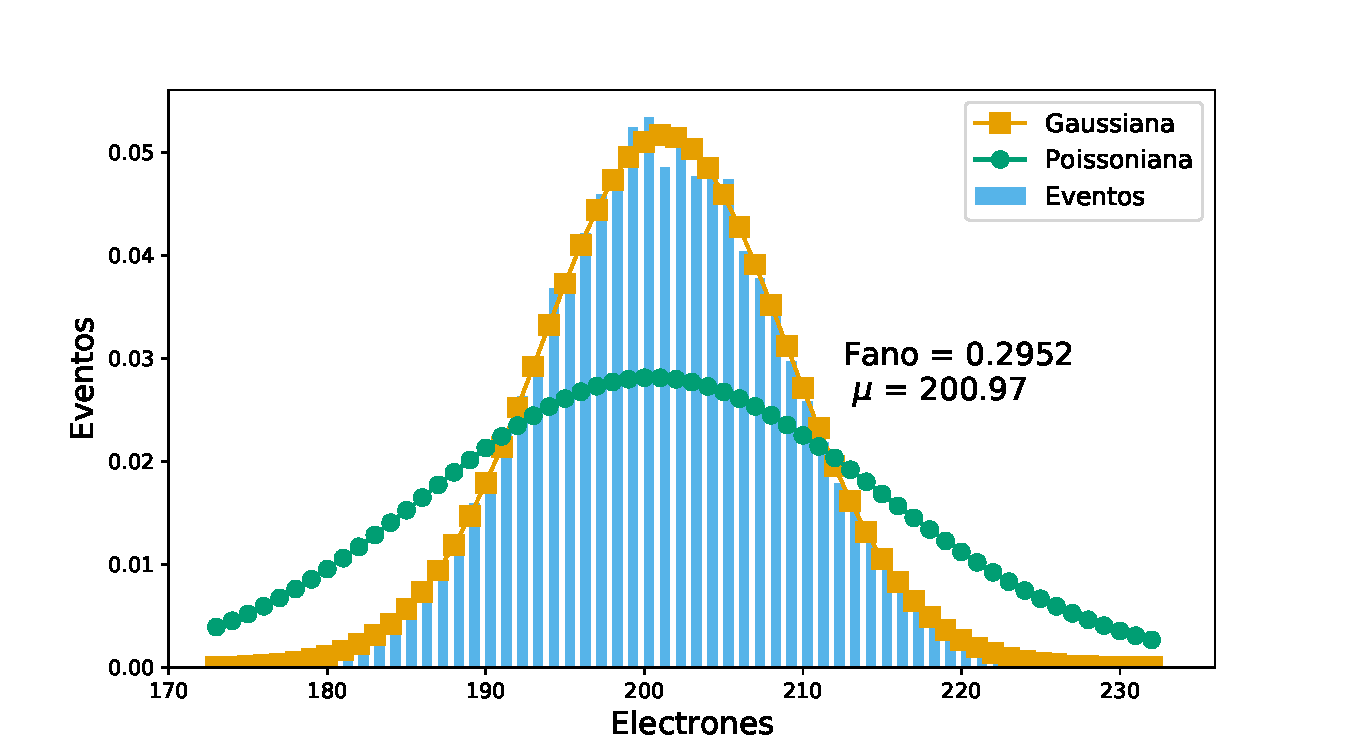
\includegraphics[scale=0.35]{Figs/Orden0_fano0.pdf}
    \caption{\footnotesize{Como reproducir esta imagen: Directorio (base) igna@Igna:~/Escritorio/Tesis2021/simulacion electrones\$ y correr ./SimuC2PyandPlot.py con parámetros: trials = 20000, distancia = 30000, atraviesa = 0 y branch git Master}}
    \label{fig:SimulacionOrden0Fano0}
\end{figure}

\begin{figure}[H]
%Para hacer este gráfico hay que correr el script que está en esta carpeta /home/igna/Escritorio/Tesis2021/Figs/Figuras_Apendice_Simulaciones/pys_para_plots y se llama Orden0_simu_SI_atraviesa.py con los datos de esta carpeta /home/igna/Escritorio/Tesis2021/Figs/Figuras_Apendice_Simulaciones/txts_para_plots y se llama orden0_simu_SI_atraviesa.txt
    \centering
    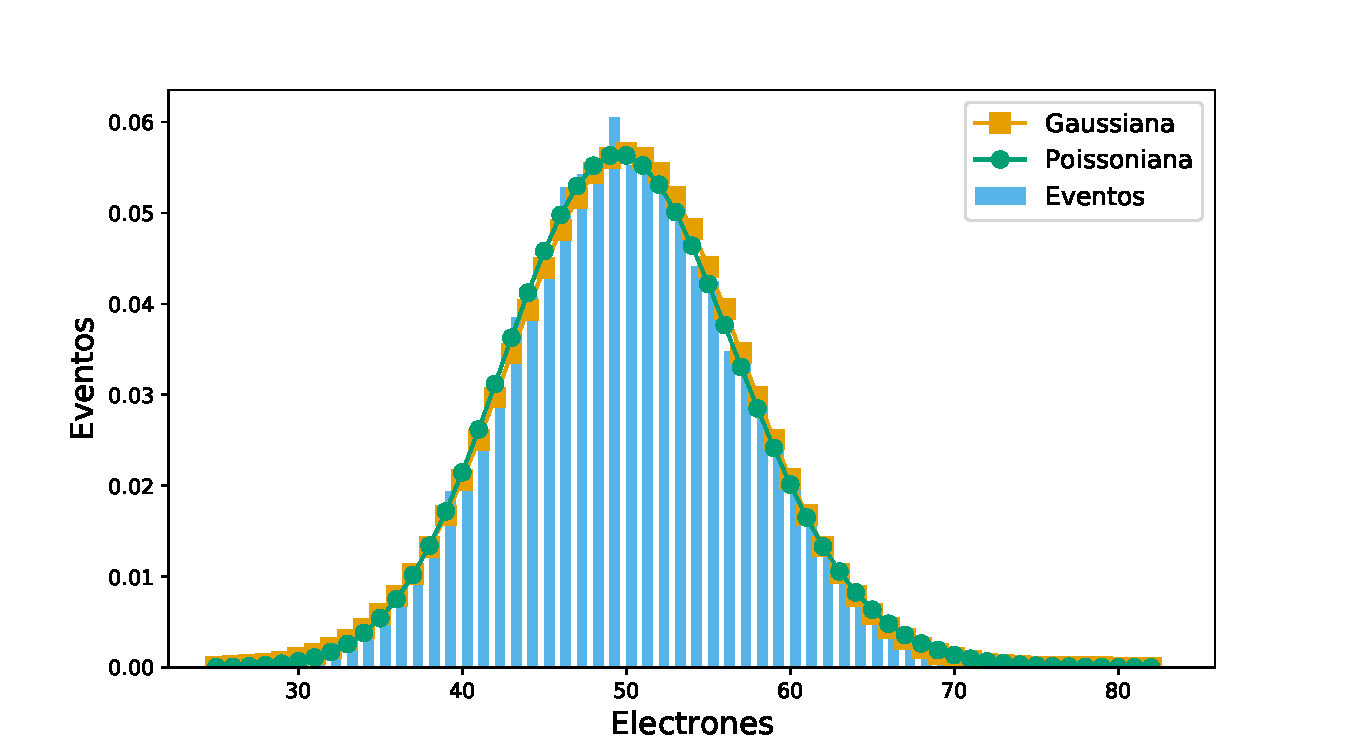
\includegraphics[scale=0.35]{Figs/Orden0_fano1.pdf}
    \caption{\footnotesize{Como reproducir esta imagen: Directorio (base) igna@Igna:~/Escritorio/Tesis2021/simulacion electrones\$ y correr ./SimuC2PyandPlot.py con parámetros: trials = 20000, distancia = 5000, atraviesa = 0 y branch git Master}}
    \label{fig:SimulacionOrden0Fano1}
\end{figure}
\noindent Si bien este modelo de juguete es una sobre-simplificación del proceso de dispersión real, los resultados de este están en concordancia con la hipótesis de que el factor de Fano es menor a $1$ debido a que la partícula incidente deposita toda su energía en el material.\\
\indent Con el fin de explorar mejor esta hipótesis, se propuso mejorar el modelo de la simulación Montecarlo. Esta vez considerando la posibilidad de que la partícula incidente pierda energía, además de por ionización, por emisión de fonones de la red. En este sentido se combinaron ideas de los trabajos de R.C. Alig et al.\cite{Alig} y K. Ramanathan \cite{Ramanathan}. En el primero proponen un modelo en el que la partícula incidente interactúa con el material, generando pares electrón-hueco por ionización en forma de cascada y, eventualmente, perdiendo energía por emisión de fonones. La forma en el que la partícula incidente va perdiendo energía depende fuertemente de la energía que tiene al momento de generar un par electrón-hueco. Esta dependencia está modelada en el segundo trabajo y lo llaman \textit{modelo simplificado}, donde proponen que la energía $E$ que se transfiere a para generar pares electrón-hueco se reparte según una distribución Beta, de la forma
\begin{equation*}
    p(x|\alpha) = \frac{2}{B(\alpha)} x^{\alpha - 1}(1-x)^{\alpha - 1}
\end{equation*}
donde $x = \frac{E}{E_{r} - E_{g}}$ es la variable aleatoria, con $E_{r}$ la energía inicial de la partícula en cada ionización, $E_{g}$ es la energía del gap del Silicio y $E$ es la fracción de energía va a parar a un nuevo par electrón hueco. Utilizando esta distribución para generar realizaciones de la variable aleatoria $x$, se puede despejar el valor de $E$ que es la energía transferida para generar pares electrón-hueco, para este modelo. Por otro lado, $B(\alpha)$ es la función Beta con un único parámetro $\alpha$, y viene dada, para el caso general por
\begin{equation*}
    B(\alpha, \beta) 
    = \frac{\Gamma(\alpha)\Gamma(\beta)}{\Gamma(\alpha) + \Gamma(\beta)}
\end{equation*}
y, para este caso particular, el parámetro $\beta = \alpha$ y $\alpha$ es el parámetro dependiente de la energía $E_{r}$ que determina el régimen de distribución de la energía, o en otras palabras, la forma de la distribución. \\
\indent La razón de la utilización de la distribución Beta para modelar como se reparte la energía en la generación de pares electrón-hueco por ionización:
\begin{itemize}
    \item \textbf{A bajas energías de la partícula incidente}, se tienen distribuciones muy picudas en los extremos posibles: $E = 0$ y $E = E_{R}+E_{g}$,
    \item \textbf{A energías mucho mayores que la energía del gap}, $E_{R} >> E_{g}$: Se tiene una distribución aproximadamente uniforme,
    \item \textbf{A energías entre $3.4\,eV$ - $4.2\,eV$ } se tiene una distribución de energía muy picuda en el medio de $x = E/(E_{R} - E_{g})$.
\end{itemize}
y estos tres casos pueden resumirse utilizando la Beta con el parámetro $\alpha$ adecuado. Para energías bajas, el parámetro $\alpha$ tiende a cero y se tiene una distribución con máximos en los extremos del intervalo. Para energías entre $3.4\,eV$ y $4.2\,eV$ se tiene una distribución con un máximo en el medio del intervalo y el parámetro $\alpha$ puede tender a infinito. Por último, para energías mucho mayores a la energía del gap, el parámetro $\alpha = 1$ y la distribución es uniforme. Estos casos se resumen el gráfico de la figura \ref{fig:BetaDist}.
\begin{figure}[H]
% Este gráfico se hace con el script que está acá: /home/igna/Escritorio/Tesis2021/Figs/Figuras_Apendice_Simulaciones/pys_para_plots DistBetaFig.py
    \centering
    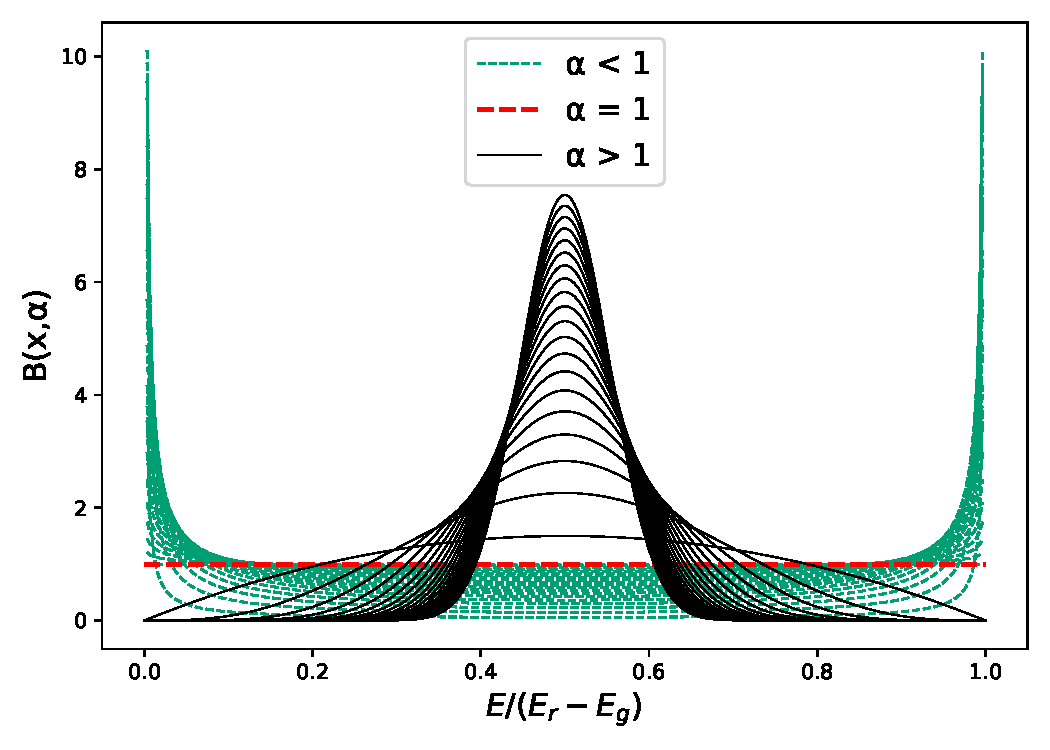
\includegraphics[scale=.7]{Figs/BetaDistFig.pdf}
    \caption{\footnotesize{Distribución Beta para diferentes valores del parámetro $\alpha$}}
    \label{fig:BetaDist}
\end{figure}

\subsection{Orden uno}
\noindent Utilizando ideas tomadas de los trabajos anteriormente citados, se realizaron simulaciones Montecarlo para intentar reproducir el mecanismo de creación de pares electrón-hueco por ionización. Para este caso se tuvo en cuenta la posibilidad de disipación de energía por emisión de fonones, a una energía fija de $\hbar\omega_{0} = 0.063\,eV$.\\
\indent El mecanismo de cascada por el cual se producen las ionizaciones consiste en que para una dada energía inicial $E_{R}$, una fracción de esa energía se utiliza para generar un par electrón-hueco y la energía restante vuelve a fraccionarse para generar otros pares electrón-hueco. Estos pares generados, a su vez, utilizan fracciones de esa energía que les fue entregada para generar otros pares, en un proceso que se repite hasta que la energía disponible para repartir en cada rama de la cascada es menor a la energía del gap del Silicio y no es suficiente para generar más pares. Durante todo este proceso existe una probabilidad no nula de que parte de la energía se pierda por emisión fonones en la red.\\
\indent Se define una probabilidad $P_{eh}$ para la cual se produce ionización y una probabilidad $1 - P_{eh}$ para la cual se produce emisión de fonones. Esta probabilidad depende de la energía inicial, al igual que el parámetro $\alpha$ de la distribución Beta, y viene dada por
\begin{equation}
    P_{eh}(E_{R}) = 
    \left[
        1 + \frac{\Gamma_{ph}(E_{R})}{\Gamma_{eh}(E_{R})}
    \right]^{-1}
        \label{ec:ProbabilidadIonizacion}
\end{equation}
donde 
\begin{equation*}
    \frac{\Gamma_{ph}(E_{R})}{\Gamma_{eh}(E_{R})}
    = A\frac{105}{2\pi}\frac{(E_{R} - \hbar \omega_{0})^{1/2}}{(E_{R} - E_{g})^{7/2}}
\end{equation*}
con $A = 5.2\,eV^{3}$, que es una constante fenomenológica que contiene información microscópica del sistema y que además puede ajustarse para reproducir valores medidos experimentalmente. Por otro lado, $\Gamma_{ph}$ y $\Gamma_{eh}$ son las tasas de producción de fonones y pares electrón-hueco, respectivamente.\\
\indent El resultado de la simulación es simplemente el número de pares ionizados a partir de la energía inicial $E_{R}$. De esta puede verse la distribución de la cantidad de pares generados y además calcular tanto su varianza como su esperanza, para así obtener el factor de Fano.\\
\indent Otro factor a tener en cuenta en la simulación es la conservación de la energía durante el proceso de creación de pares. Puede considerarse que la energía transferida al ionizar, puede utilizarse totalmente para ionizar otros pares, o puede considerarse que siempre que se de una ionización, habrá una pequeña parte de energía que se pierde y no puede ser utilizada, es decir, que no se conserva la energía.\\
\indent Por último, en este tipo de simulación solo se puede considerar el caso en el que la partícula disipa toda su energía en el interior del material, de modo que se esperan valores para el factor de Fano menores a la unidad.

\subsubsection{Implementación}
\noindent La implementación de los códigos que ejecutan la simulación Montecarlo se realizó con los lenguajes C y Python. Con C se realiza todo el trabajo de alto costo computacional, mientras que Python cumple un rol de interfaz para los parámetros de la simulación, como ser, por ejemplo, la energía inicial, la cantidad de corridas del Montecarlo, etc.\\
\indent A grandes rasgos, en el código en C están implementadas las funciones que hacen los cálculos antes mencionados: El cálculo de la probabilidad de ionización $P_{eh}$ a partir de la expresión \eqref{ec:ProbabilidadIonizacion}, el cálculo del parámetro $\alpha = \alpha(E_{R})$ según la energía $E_{R}$ para la distribución Beta, a partir de la cual se genera una realización de la variable aleatoria de la que se puede despejar la energía transferida a un par electrón-hueco por ionización. Finalmente, por recursión se simulan los procesos de ionización en cascada y se cuenta la cantidad final de electrones ionizados.\\
\indent Por otro lado, la función del código en Python no es más ejecutar el programa en C las veces que sean necesarias y con los parámetros iniciales de interés para obtener el resultado buscado.\\
\indent Más en detalle, el programa en C consta de un total de $6$ funciones, las cuales se listan a continuación con una breve descripción de su funcionamiento
\begin{enumerate}[label=\arabic*., listparindent=1.5em]
    \item \verb|Random()|: Es simplemente una función que genera realizaciones \verb|p_rand| de una distribución uniforme, entre $0$ y $1$. Se usa para generar una probabilidad de comparación en el Montecarlo.
    \item \verb|Peh(E_r, A)|: Es la función encargada de realizar el cómputo de la probabilidad de ionización, según la ecuación \eqref{ec:ProbabilidadIonizacion}, a partir de la energía $E_{R}$, que es un parámetro inicial que es ingresado con Python. Esta probabilidad \verb|p_eh| se compara con \verb|p_rand| en el algoritmo de aceptación del Montecarlo.
    \item \verb|alpha(E_r)|: Calcula el valor del parámetro $\alpha$ en base al valor del parámetro \verb|E_r|. Si bien el parámetro \verb|E_r| es un parámetro inicial, que para el Flúor es $677\,\si{eV}$, a medida que evoluciona el sistema, la energía se va perdiendo en ionizaciones y este parámetro es actualizado. Con cada actualización se calcula nuevamente el valor de $\alpha$ de para la distribución Beta. El valor del parámetro se calcula entonces como
    \begin{equation*}
        \alpha =
        \left\{
            \begin{matrix}
                0.1\ \mbox{si}\ E_{r} < E_{g}\\
                1\ \mbox{si}\ E_{g} < E_{r} < 2E_{g}\\
                1\ \mbox{si}\ 3.4\,\si{eV} < E_{r} < 4.2\,\si{eV}\\
                0.0207E_{r} + 0.95435\ \mbox{en otro caso.}
            \end{matrix}
        \right.
    \end{equation*}
    \item \verb|evolucionar(E_r, A, E_loss, rand_beta)|: Genera la evolución del sistema mediante Montecarlo, haciendo uso de las funciones anteriores. Implementa un bucle \verb|while|, cuya condición es que se repita el proceso mientras que la energía \verb|E_r| sea mayor que la energía del gap del Silicio \verb|E_g|. Dentro del bucle se calcula la probabilidad \verb|p_eh| de ionización, el parámetro $\alpha$, que luego es usado para generar un número pseudo aleatorio con distribución Beta del cual despejar la fracción de energía \verb|E_traf| que va a un par electrón hueco al ionizar y, por último, genera el número pseudo aleatorio de distribución uniforme con cual comparar la probabilidad de ionización en el Montecarlo.\\
    \indent Una vez que se tienen estos valores, siempre y cuando se cumpla que la probabilidad de ionizacion \verb|p_eh| sea mayor que \verb|p_rand| y que al mismo tiempo la fracción de energía \verb|E_tranf| sea mayor que $3.75\,\si{eV}$\footnote{Condición que cobra gran relevancia en los resultados y se explica en más datella en la siguiente sección} (valor medio para la energía de creación electrón hueco $\varepsilon_{\eh}$), entonces se actualiza el valor de la energía inicial \verb|E_r| restándole la fracción de energía transferida. Además, también, se guardan en una lista la resta entre las energías transferidas \verb|E_r| y la energía perdida por ionización \verb|E_loss|. Esta última es un parámetro configurable de la simulación, en la cual se puede considerar el caso donde la energía se conserva y \verb|E_loss = 0| o el caso en el que no hay conservación de energía y \verb|E_loss|$\neq$\verb|0|. Notar que la cantidad de elementos de la lista será la cantidad de pares electrón-hueco generados por una rama de la cascada con energía inicial \verb|E_r|. Luego, cada elemento de la lista se transforma, para otra rama, en \verb|E_r|, generando una nueva lista. Repitiendo con todas las energías de toda la lista y todas las sublistas, se pueden contar los electrones ionizados.\\
    \indent De no cumplirse la condición del Montecarlo, el sistema pierde energía por emisión de fonones, es decir, la energía \verb|E_r| se actualiza restándole un valor fijo de energía $\hbar \omega = 0.063\,\si{eV}$. El resultado de esta función es una lista con las energías de una sola rama de la cascada.
    \item \verb|recursion(E_r, A, E_loss, rand_beta)|: Esta función cuenta de manera recursiva la cantidad de electrones ionizados durante la cascada. La recursion, en este caso, tiene la ventaja de que es muy sencilla de implementar, pero tiene como desventaja que no es tan sencillo entender por qué funciona correctamente.\\
    \indent Lo primero que hace esta función es generar una lista energías, \verb|Energia|, llamando a la función \verb|evolucionar()| y luego se itera sobre todas estas, contando la cantidad total de elementos que posee. Esas energías son las que fueron usadas para ionizar un par electrón hueco, así que la cantidad de energías que alberga la lista es equivalente a la cantidad de pares generados. Notar que a \verb|recursion()| se le pasa como argumento \verb|E_r|. De modo que si dentro de \verb|recursion()| se vuelve a llamar a ella misma, pero ahora en vez de usar como argumento \verb|E_r|, se usa el primer elemento de la lista \verb|Energia|, es decir \verb|Energia[0]|, se produce una nueva lista a partir de una energía inicial menor y contando la cantidad de elementos. Si ahora se repite para el elemento \verb|Energia[1]|, se genera otra lista de energías. El proceso se repite hasta que todas las energías de la lista original se agotaron. Luego, las sublistas generadas repiten el proceso para todos sus elementos hasta que eventualmente la energía de las listas no es suficiente para seguir ionizando y el proceso termina.\\
    \indent El valor de salida de la función \verb|recursion()| es un entero y contabiliza la cantidad de elementos encontrados en la lista, es decir, la cantidad de electrones ionizados. Durante el proceso de recursión se van sumando todas las cantidades de carga ionizada en cada paso y finalmente se obtiene la carga total generada durante la cascada.
    \item \verb|main()|: Esta se encarga de llevar adelante las repeticiones del experimento con el fin de obtener estadística. Además, en esta se definen los parámetros necesario para la simulación, como ser la energía inicial \verb|E_r|, el parámetro \verb|A|, el valor de la energía que se pierde por ionizar \verb|E_loss|, la cantidad de experimentos que se quieren realizar \verb|trials| y la generación de un archivo \verb|.txt| con los datos obtenidos para ser levantados posteriormente con Python.
\end{enumerate}
Cabe destacar que de esta simulación el único resultado que se obtiene es la distribución de carga para una dada energía inicial $E_{r}$. Es decir, no puede conocerse ningún proceso intermedio o la \textit{historia} del proceso, solo la cantidad total de electrones generados.

\subsubsection{Simulaciones}
\noindent Se realizaron las simulaciones partiendo de una energía inicial $E_{r} = 677\,\si{eV}$, correspondiente a los rayos $X$ de Flúor, que es el principal objeto de estudio de este trabajo. Los valores de los parámetros fueron extraídos de la bibliografía y son $A = 5.2\,\si{eV}^{3}$, la energía del gap $E_{g} = 1.1\,\si{eV}$, la energía de creación electrón-hueco promedio $\varepsilon_{eh} = 3.75\,\si{eV}$ y la energía perdida cada vez que se emiten fonones $\hbar \omega = 0.063\,\si{eV}$. El resto de los parámetros son configurables y se variaron para ver los diferentes resultados de la simulación, como ser la pérdida de energía al ionizar $E_{loss}$ y la cantidad de repeticiones del experimento \textit{trials}. La simulaciones se efectuaron con no menos de $5000$ repeticiones y con diferentes valores de $E_{loss}$.\\
\indent Se simuló el proceso de cascada con con diferente cantidad de \textit{trials}, es decir, de repeticiones del experimento, partiendo desde $5000$ hasta incluso $100000$ para asegurar la robustez de la estadística. Además, con el fin de poder caracterizar mejor las dependencias entre parámetros en la simulación, se hizo un barrido sobre la pérdida de energía $E_{loss}$ para conocer la dependencia de los resultados respecto de este, partiendo desde $0\,\si{eV}$ de pérdida de energía hasta $7\,\si{eV}$ de pérdida de energía por cada ionización (equivale a perder casi $4$ veces la energía del gap del Silicio).\\
\indent Con estos barridos se vio la dependencia de tanto del factor de Fano, como de la energía de creación electrón-hueco y del valor medio de carga ionizada al variar el valor de la energía que se pierde con cada ionización. Se observó que estos parámetros son muy sensibles a la pérdida de energía del sistema, obteniéndose resultados con cambios de regímenes muy pronunciados, particularmente, cuando la energía perdida por ionización coincide con el valor $E_{loss} = 3.75\,\si{eV}$, que casualmente es la energía de creación electrón-hueco promedio y que se usó en la simulación como un parámetro fijo en la función \verb|evolucionar()|.

\subsubsection{Resultados}
\noindent Los resultados de las simulaciones del factor de Fano se ven en los gráficos de las figuras \ref{fig:Simulacion1rden1Fano1} y \ref{fig:Simulacion1rden1Fano2}. Ambos muestran la distribución de carga simulada, un ajuste Gaussiano a ese histograma, usando el $\mu$ y el $\sigma$ generado a partir de los datos y a su vez la forma de la Poissoniana que corresponde a ese valor medio $\mu$. Se ve claramente como la distribución de carga está lejos de parecerse a una distribución de Poisson y por ello el factor de Fano se aleja de la unidad.\\
\indent El primer caso corresponde a una simulación en la que se repitió el mismo experimento de cascada $100000$ veces para tener una buena robustez estadística, mientras que en el segundo caso se usaron $10000$ repeticiones del experimento. En la figura \ref{fig:FanoConvergencia} se observa la convergencia de los valores del factor de Fano a medida que aumenta el número de experimentos.
\begin{figure}[h]
%Este gráfico se puede hacer con el script GrafFanoConvergencia.py que esta en este directorio /home/igna/Escritorio/Tesis2021/Figs/Figuras_Apendice_Simulaciones/pys_para_plots
    \centering
    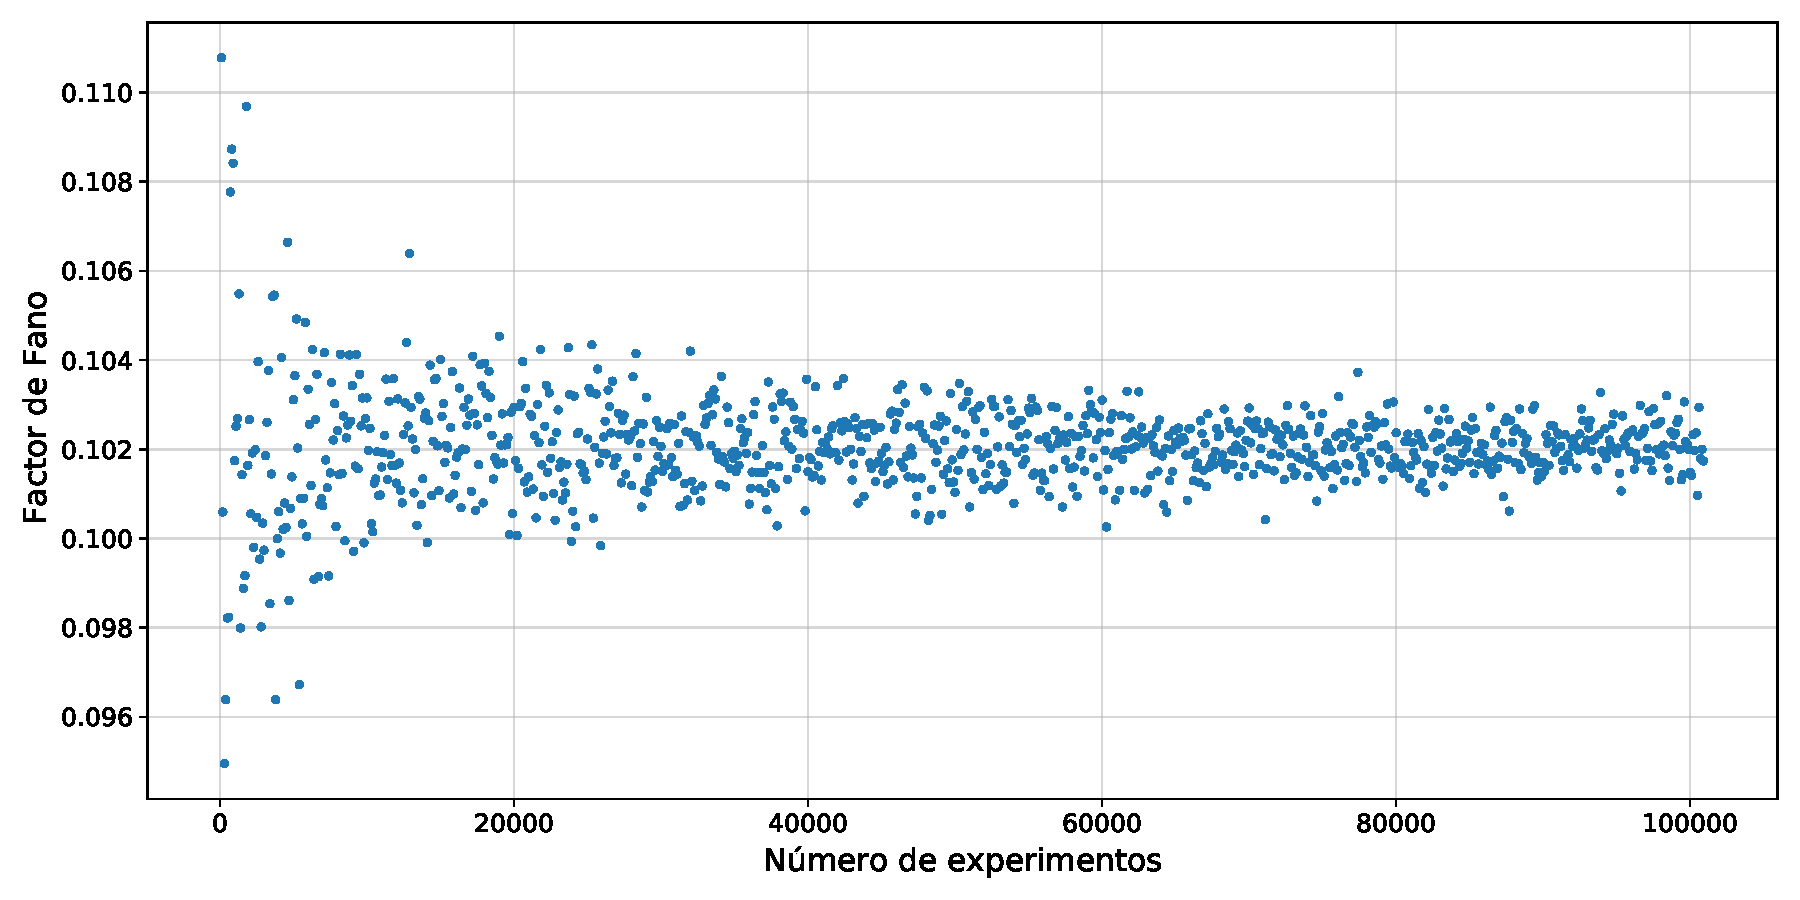
\includegraphics[scale=0.5]{Figs/FanoConvergencia.pdf}
    \caption{\footnotesize{Dispersión de los valores del Factor de Fano cada cantidad de repeticiones del experimento, partiendo desde $100$ repeticiones hasta 100900 repeticiones.}}
    \label{fig:FanoConvergencia}
\end{figure}
Para $10000$ repeticiones se ve que los valores del factor de Fano están acotados entre $\sim 0.106$ y $\sim 0.098$, mientras que para $100000$ repeticiones están acotados entre $\sim 0.104$ y $\sim 0.100$. Se nota claramente la mejora en la estadística.\\
\indent En la figura \ref{fig:Simulacion1rden1Fano1} se puede ver lo bien que se ajusta una distribución Gaussiana al histograma. En este caso el factor de Fano correspone a $F = 0.1021$ y el valor medio de carga $\mu = 192$, un valor bastante corrido a la derecha respecto del valor esperado, cercano a $\mu = 181$.
\begin{figure}[h]
%Los datos para este gráfico están en /home/igna/Escritorio/Tesis2021/Figs/Figuras_Apendice_Simulaciones/txts_para_plots Distribucion_carga_simulada_100k.txt Para modificar el graf hay que correr el .py que están en /home/igna/Escritorio/Tesis2021/Figs/Figuras_Apendice_Simulaciones/pys_para_plots Fano_100k_dist_carga.py
    \centering
    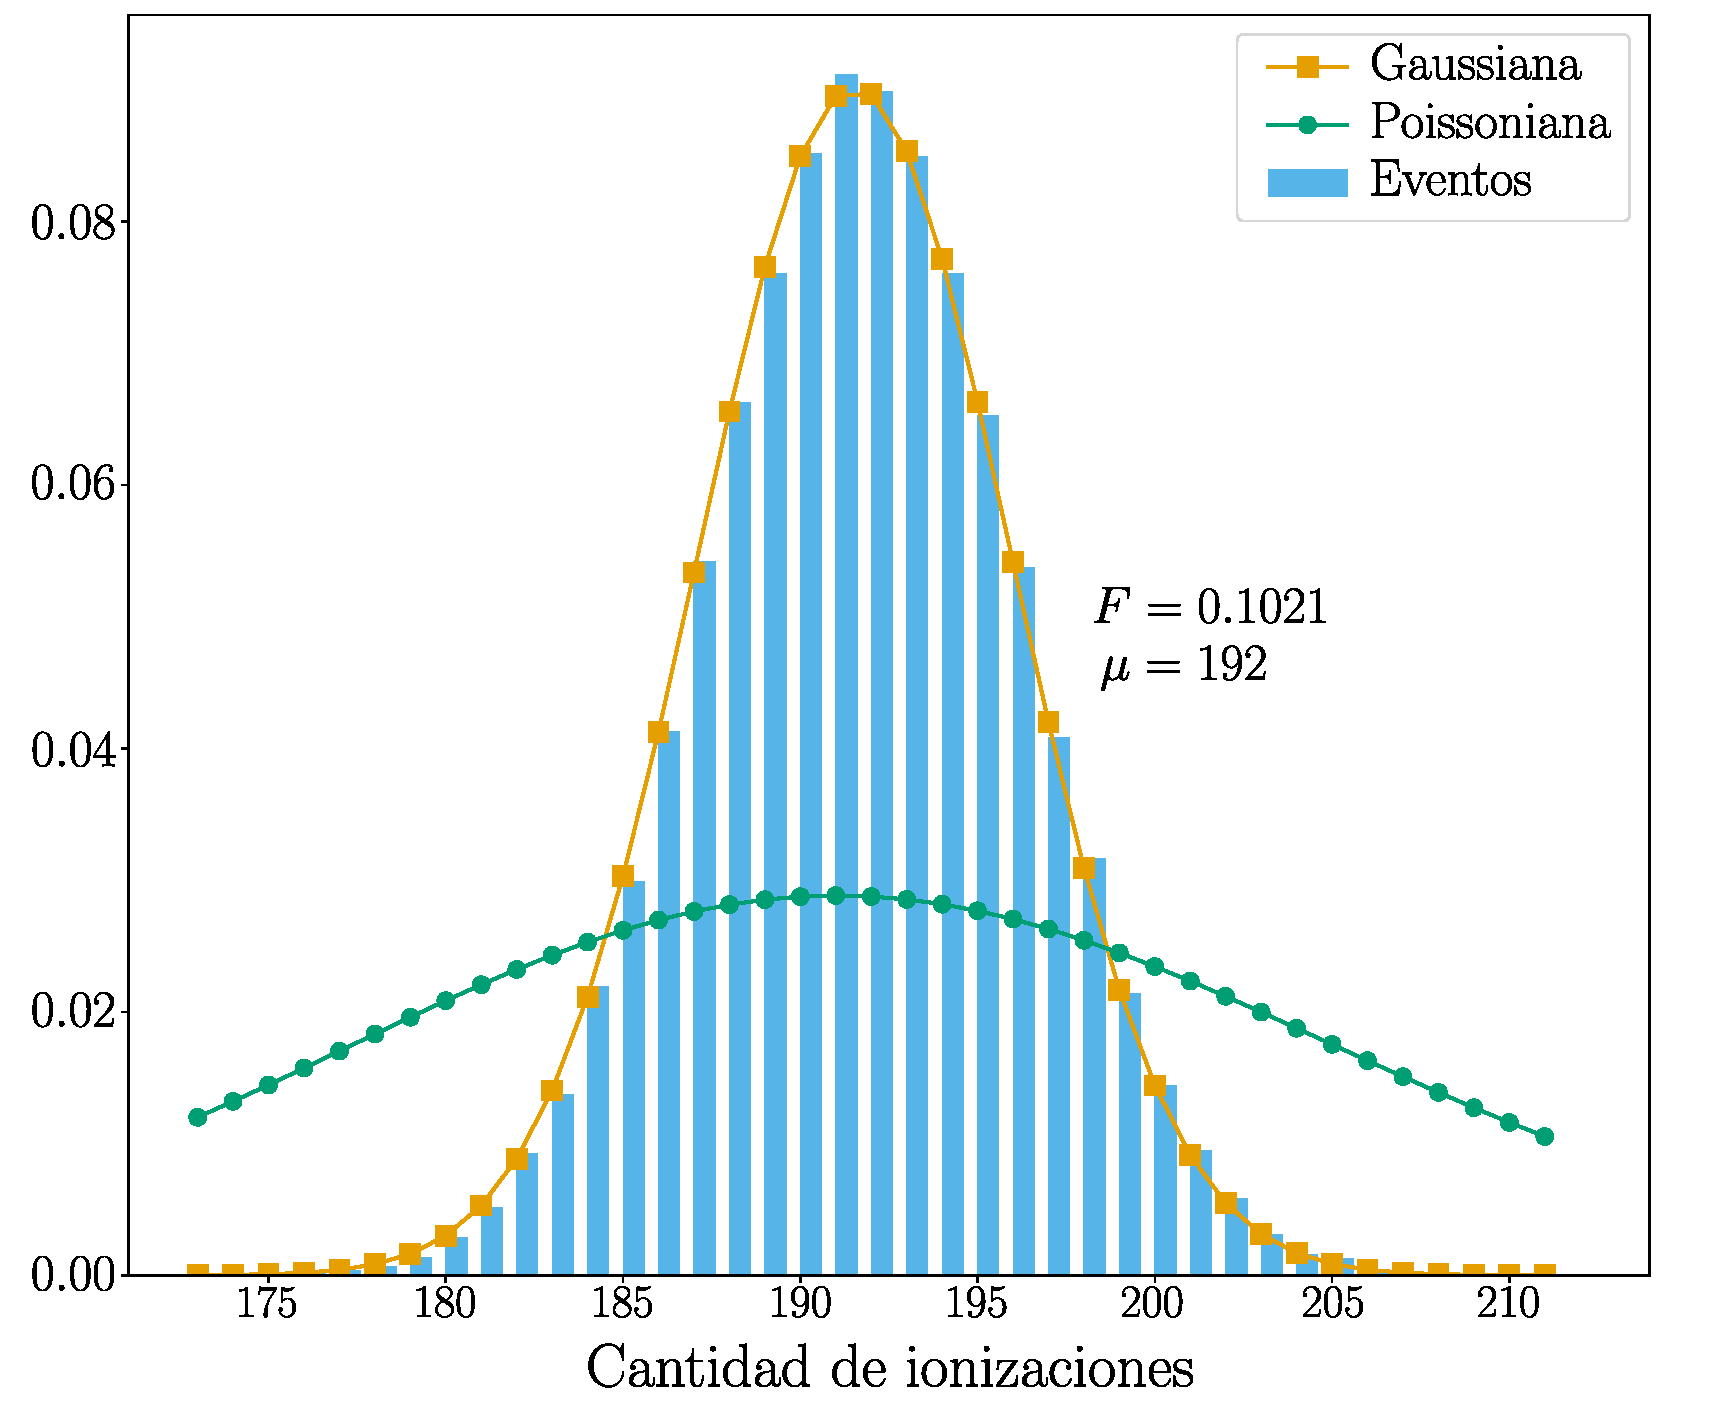
\includegraphics[scale=0.35]{Figs/Fano_677_Eloss0_100ktrials.pdf}
    \caption{\footnotesize{Distribución de carga simulada con el método de Montecarlo, con parámetro $A = 5.2\,\si{eV}^{3}$ y $100000$ \textit{trials} para obtener la mejor estadística posible. Se observa un valor medio $\mu = 192$, lo cual representa un corrimiento hacia la derecha del valor esperado para el pico de los rayos $X$ del Flúor, que es al rededor de $181$ electrones.}}
    \label{fig:Simulacion1rden1Fano1}
\end{figure}
\noindent Para el segundo caso, en la figura \ref{fig:Simulacion1rden1Fano2}, se modificó el valor del parámetro $A$ de forma que el pico coincida con lo esperado, que son $\mu = 181$ electrones. El valor de $A$ que cumple esa condición es $A = 20\,\si{eV}^{3}$, valor $5$ veces mayor al propuesto en la bibliografía para describir macroscópicamente las propiedades del Silicio.
\begin{figure}[h]
%Los datos para este gráfico están en /home/igna/Escritorio/Tesis2021/Figs/Figuras_Apendice_Simulaciones/txts_para_plots Distribucion_carga_simulada_10k.txt Para modificar el graf hay que correr el .py que están en /home/igna/Escritorio/Tesis2021/Figs/Figuras_Apendice_Simulaciones/pys_para_plots Fano_10k_dist_carga.py
    \centering
    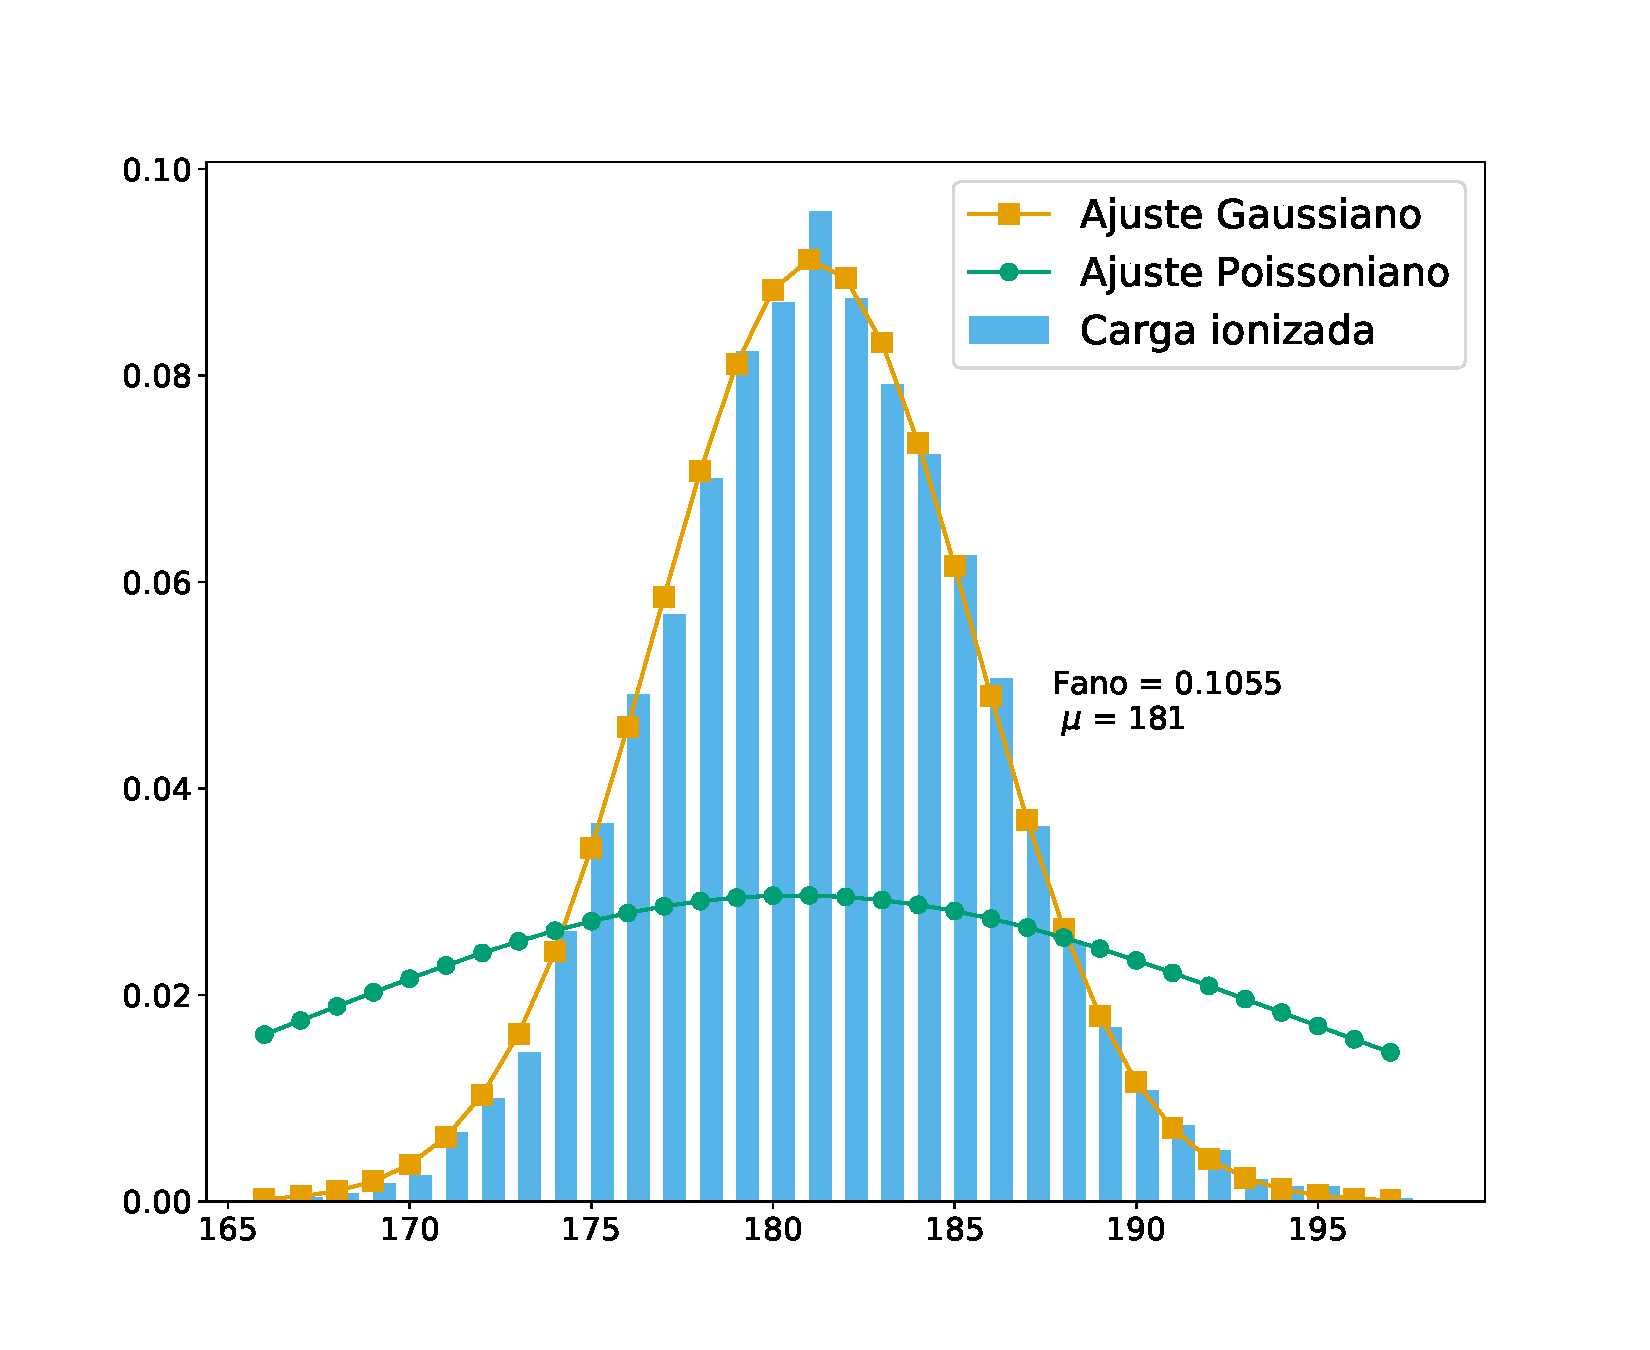
\includegraphics[scale=0.35]{Figs/Fano_677_Eloss0_10ktrials.pdf}
    \caption{\footnotesize{Distribución de carga simulada con el método de Montecarlo, forzando el parámetro $A$ para que el pico se encuentre en los $181$ electrones esperados para los $677\,\si{eV}$ de energía de los rayos X del Flúor. En este caso $A=20$ y se usaron solamente $10000$ \textit{trials}.}}
    \label{fig:Simulacion1rden1Fano2}
\end{figure}
El factor de Fano en este caso es de $F = 0.1055$, que está contenido entre las bandas esperadas para la cantidad de estadística utilizada en esta simulación. La razón por la cual usar menor estadística en este caso fue porque no era necesaria tanta robustez.\\
\indent En ambos casos el valor del factor de Fano es muy semejante y da, como se esperaba, alrededor de un orden de magnitud inferior a la unidad. Los valores esperados son << buscar valores esperados >>.\\
\indent En cuanto a los barridos, la dependencia del factor de Fano con la energía $E_{loss}$ (y al igual que la energía de creación electrón-hueco y el valor medio de carga ionizada) presenta un cambio de régimen abrupto cuando se cruza el umbral $E_{loss} = 3.75\,\si{eV}$. En la figura \ref{fig:FanoVsEloss} puede verse claramente este cambio de régimen. También se observa que cuando hay conservación de la energía, es decir, $E_{loss} = 0$, es cuando se obtiene un factor de Fano más semejante al observado experimentalmente, que está cerca de $0.1$.
\begin{figure}[h]
%a) Esta figura se puede hacer con los datos de: fano_Eloss_mu_vec.txt que está en el directorio /home/igna/Escritorio/Tesis2021/Figs/Figuras_Apendice_Simulaciones/txts_para_plots usando el .py Barridos_mu_Eloss_fano.py que está en /home/igna/Escritorio/Tesis2021/Figs/Figuras_Apendice_Simulaciones/pys_para_plots
    \centering
    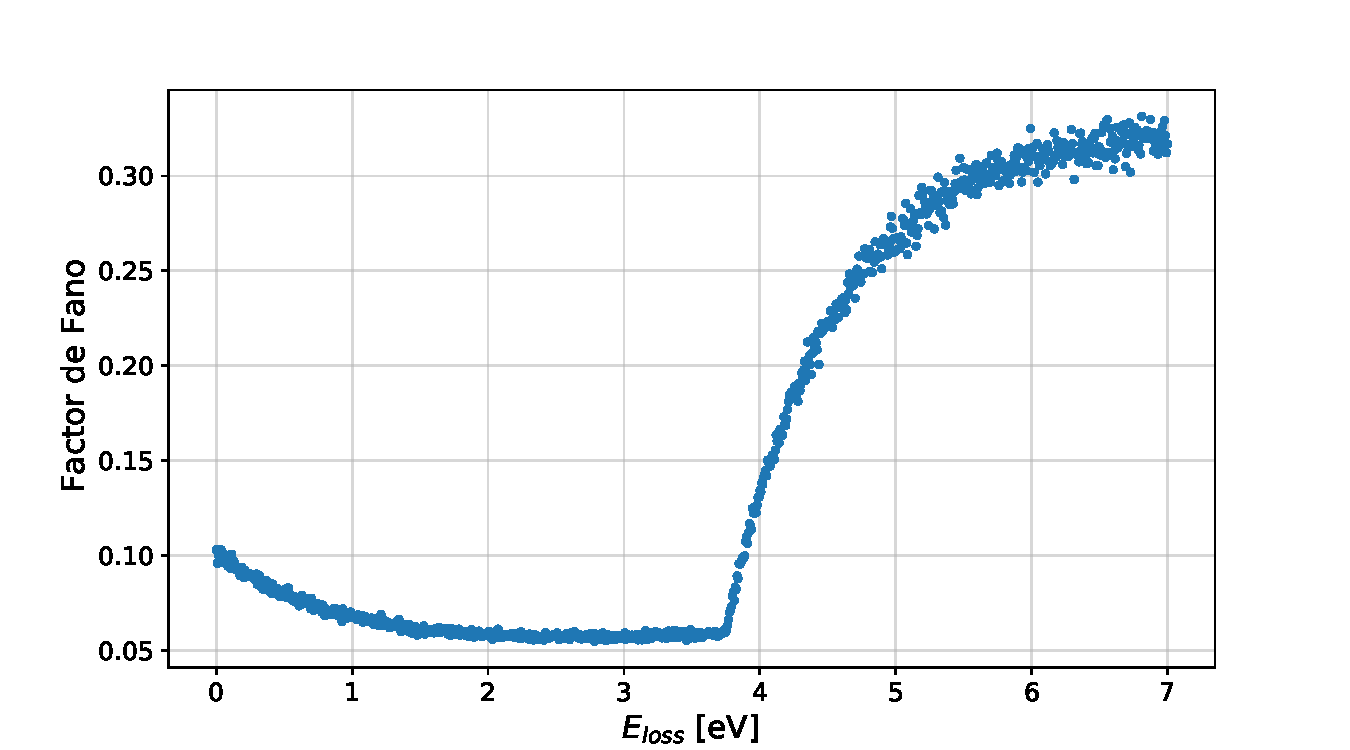
\includegraphics[scale=0.35]{Figs/Fano_vs_Eloss_5ktrials_0-7Eloss.pdf}
    \caption{\footnotesize{asd.}}
    \label{fig:FanoVsEloss}
\end{figure}
A medida que aumenta la pérdida de energía, el factor de Fano comienza a decrecer hasta que se alcanza los $3.75\,\si{eV}$ de pérdida de energía, donde se observa el cambio brusco en la curva, y se observa un aumento pronunciado de la misma, muy semejante a un punto crítico.\\
\indent De la misma forma, el valor media de la carga ionizada $\mu$ tiene un cambio de concavidad en la curva a medida que aumenta la cantidad de energía perdida por cada ionización, como se ve en la figura \ref{fig:ElossVsMu}

\begin{figure}[h]
% b) Esta figura se puede hacer con los datos de: fano_Eloss_mu_vec.txt que está en el directorio /home/igna/Escritorio/Tesis2021/Figs/Figuras_Apendice_Simulaciones/txts_para_plots usando el .py Barridos_mu_Eloss_fano.py que está en /home/igna/Escritorio/Tesis2021/Figs/Figuras_Apendice_Simulaciones/pys_para_plots
    \centering
    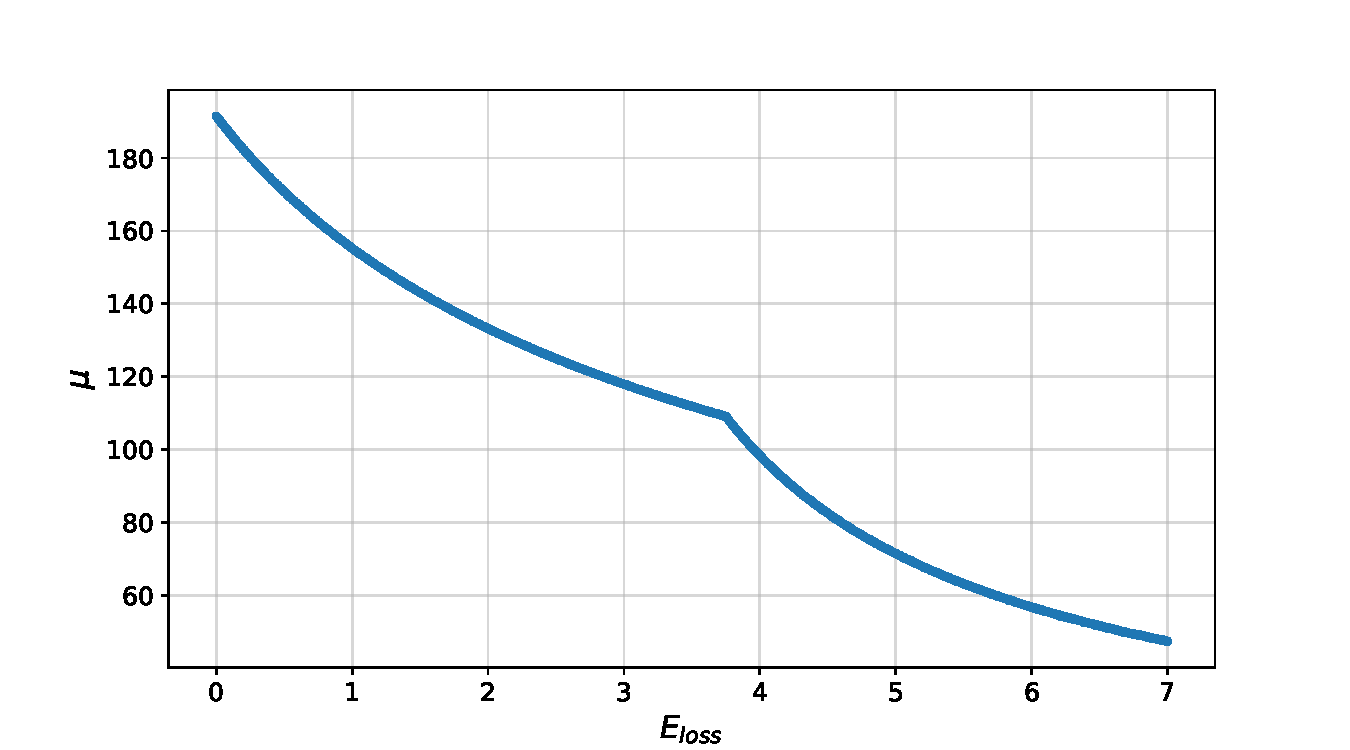
\includegraphics[scale=0.35]{Figs/ELoss_vs_mu_5ktrials_0-7Eloss.pdf}
    \caption{\footnotesize{asd.}}
    \label{fig:ElossVsMu}
\end{figure}
Nuevamente, los valores más cercanos a los medidos experimentalmente son los que corresponden a los casos en los que hay conservación de la energía.\\
\indent Por último, para la energía de creación electrón hueco, calculada a partir del valor medio de carga ionizada y la energía inicial $E_{R} = 677\,\si{eV}$, usando $\left\langle\varepsilon_{\eh} \right\rangle= 677\,\si{eV}/\mu$, claramente tendrá el mismo cambio de régimen en $3.75\,\si{eV}$, como se ve en la figura \ref{fig:CreacionHuecoVsEloss}
\begin{figure}[h]
%a) Esta figura se puede hacer con los datos de: fano_Eloss_mu_vec.txt que está en el directorio /home/igna/Escritorio/Tesis2021/Figs/Figuras_Apendice_Simulaciones/txts_para_plots usando el .py Barridos_mu_Eloss_fano.py que está en /home/igna/Escritorio/Tesis2021/Figs/Figuras_Apendice_Simulaciones/pys_para_plots
    \centering
    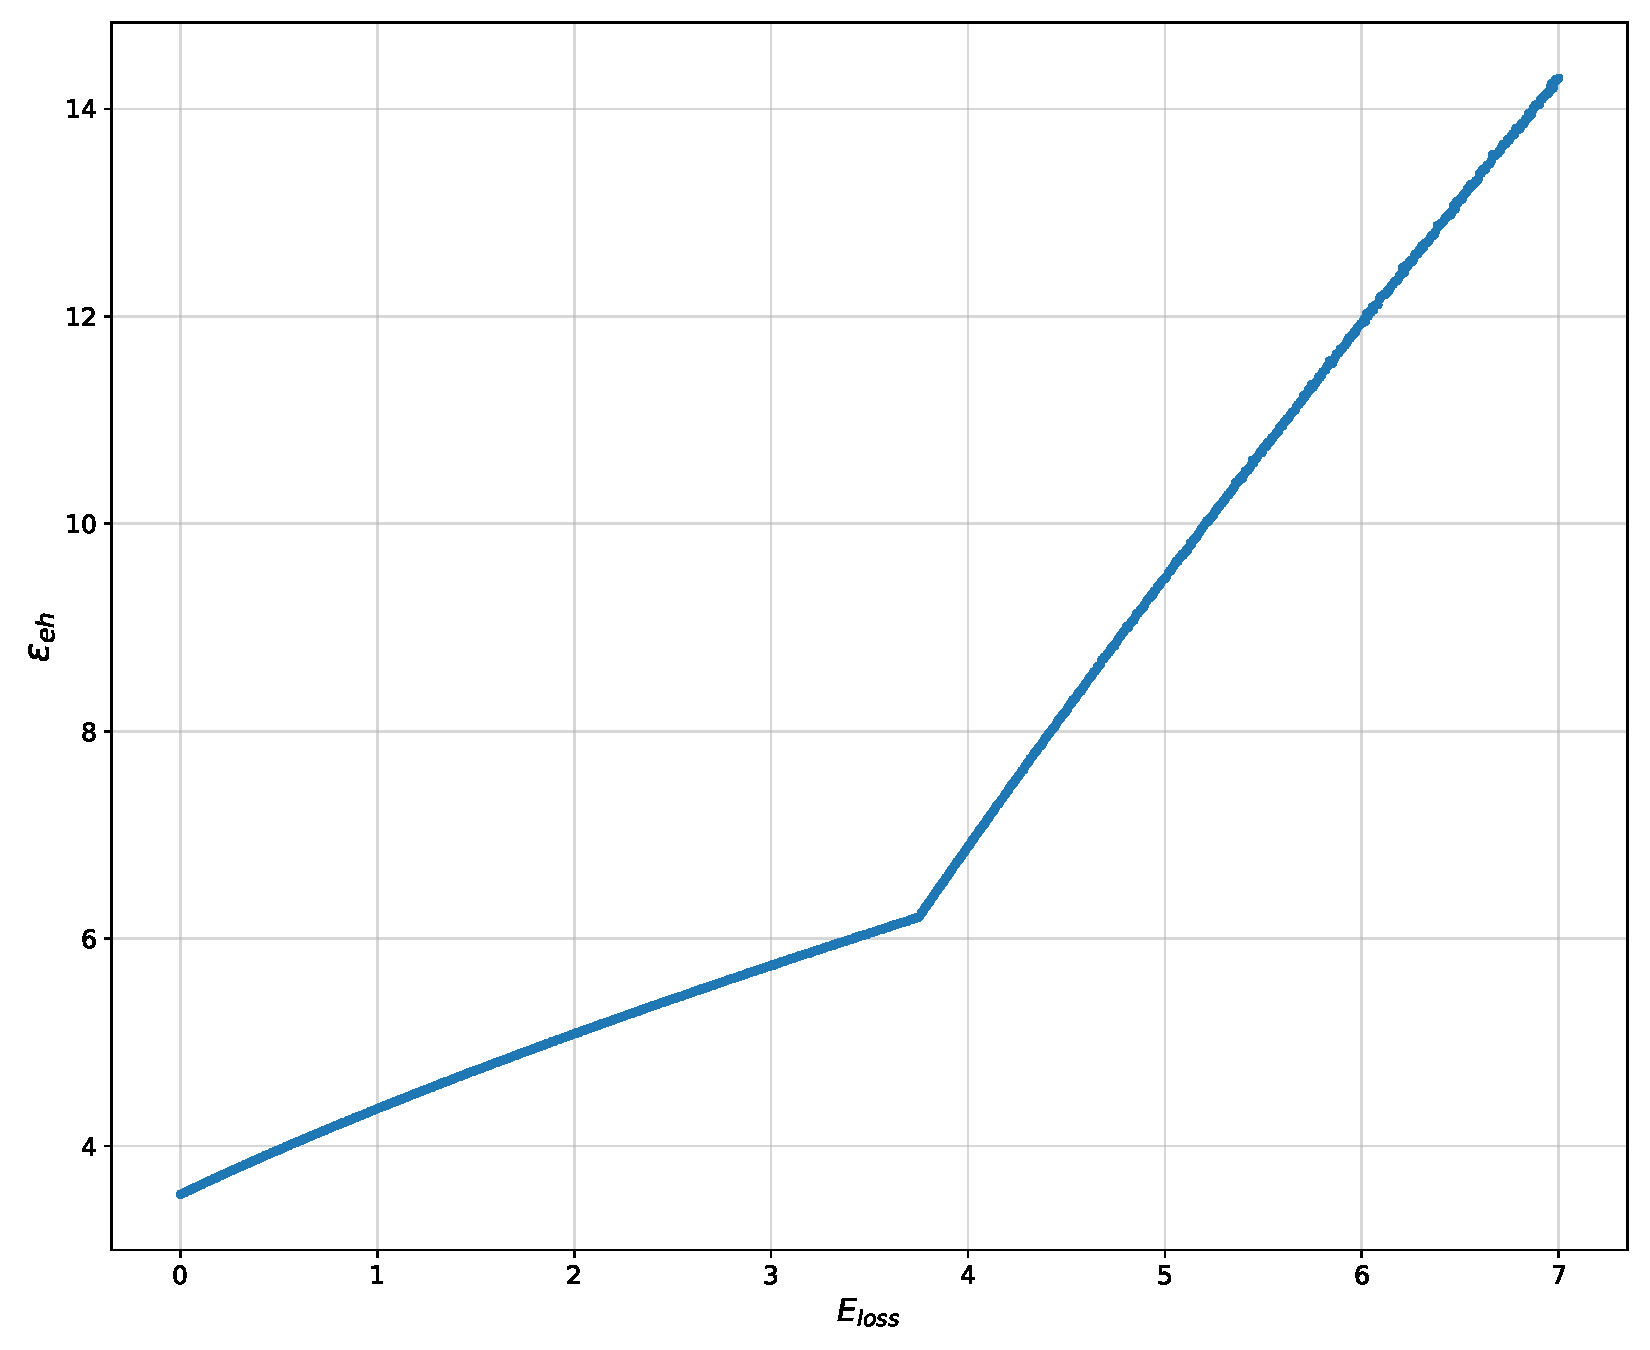
\includegraphics[scale=0.35]{Figs/E_eh_vs_Eloss_5ktrials_0-7Eloss.pdf}
    \caption{\footnotesize{asd.}}
    \label{fig:CreacionHuecoVsEloss}
\end{figure}
Con lo cual se observa que este Montecarlo \textit{de juguete} es muy sensible a dos parámetros muy importantes de la física real del sistema: La energía de creación electrón hueco, porque es el parámetro de la condición de \verb|evolucionar()| que determina si hay o no ionización; y la conservación de la energía. Se observa que cuando la energía se conserva en la simulación, se obtienen los resultados más cercanos a los observados experimentalmente y reportados en la bibliografía.

%%%%%%%%%%%%%%%%%%%%%%%%%%%%%%%%%%%%%%%%%%%%%%%%%%%%%%%%%%%%%%%%%%
%%%%%%%%%%%%%%%%%%%%%%%%%%%%%%%%%%%%%%%%%%%%%%%%%%%%%%%%%%%%%%%%%%
%%%%%%%%%%%%%%%%%%%%%%%%%%%%%%%%%%%%%%%%%%%%%%%%%%%%%%%%%%%%%%%%%%
\chapter{Resultados previos}
\noindent En trabajos previos se estudiaron las ventajas de la utilización de la novedosa tecnología \textit{skipper} CCD, para lograr medir con precisión subelectrónica en régimenes de energía donde los sensores CCD convencionales más precisos sólo podrían alcanzar resoluciones del orden de los $2$ electrones. Por primera vez fue usada para poder estimar el factor de Fano y la energía de creación electrón-hueco en el Silicio a una energía de $5.9\,\si{keV}$ y para diferentes temperaturas. Además de obtenerse las primeras estimaciones, también se trabajó sobre los desafíos que la utilización de esta incipiente tecnología representa. Por ejemplo, la calibración del detector para la transformación de las unidades analógico digitales (ADU's) a cantidad de carga, primero utilizando una calibración lineal y luego calibraciones no lineales de la forma de
\begin{equation*}
    e = ADU \times \alpha + ADU^{2} \times \beta
\end{equation*}

acá voy a hablar de la calibración absoluta que hizo kevin



%%%%%%%%%%%%%%%%%%%%%%%%%%%%%%%%%%%%%%%%%%%%%%%%%%%%%%%%%%%%%%%%%%

\chapter{Análisis preliminares y factibilidad}
\noindent En este trabajo se propone realizar un análisis profundo de las mediciones existentes del sensor, aplicando un corte de calidad a las imágenes que aumenta el número de eventos detectados por el programa, para así aumentar la estadística y mejorar la resolución con la que se calculan tanto el factor de Fano como para la energía de creación electrón-hueco. %Sin embargo, aplicar este corte de calidad trae aparejado un sesgo en el conteo de carga de cada evento, tanto por defecto como por exceso, con lo cual es un efecto que debe corregirse.
En este sentido, es de gran importancia cuantificar el aumento en la estadística al modificar los parámetros usados en el programa de reconocimiento de clusters y así poder establecer la factibilidad de la mejora en el cálculo de las incertezas de los valores antes mencionados.\\
\indent El parámetro clave en este caso se llama \verb|EPIX|, y es un valor umbral, define a partir de qué cantidad de carga se cuenta o no como un píxel vacío. Por ejemplo, para \verb|EPIX = 0.5|, todos los píxeles con carga menor o igual $1$ se cuentan como píxeles vacíos, y los que tengan carga mayor a $1$ serán contabilizados normalmente, para \verb|EPIX = 1.5|, todos los píxeles con carga menor o igual a $2$ se cuentan como píxeles vacíos y los píxeles con carga mayor a $2$ se cuentan normalmente.\\
\indent En trabajos previos\footnote{cite tesis kevin}, los valores obtenidos para el factor de Fano y energía de creación electrón-hueco, fueron calculados con un valor de \verb|EPIX = 0.5|. Se espera que al modificar este parámetro, el conteo de eventos varíe y que, en particular, aumente cuando el \verb|EPIX| aumenta. Esto se debe a que es muy común que se tenga un evento de interés, por ejemplo un clúster de $4$ píxeles de área y con una carga total de $180$ electrones, y alrededor de este se acumulen píxeles con cargas debidas a corrientes oscuras del sensor, de por ejemplo $1$ o $2$ electrones. En estos casos podría suceder que la conexión entre el clúster de interés y los píxeles con carga espuria se extiendan lo suficiente como para que el algoritmo reconozca un gran clúster con exceso de carga y sea filtrado dado que no cumple con los cortes de calidad impuestos. También podría suceder que estos píxeles con carga espuria conecten $2$ clústeres de interés, lo cual es un caso más extremo, dado que el algoritmo reconocería un único clúster de $\sim 360$ electrones, de forma que se perderían, no $1$, sino $2$ eventos que podrían aportar positivamente a la estadística. Al aplicar un umbral que elimine los píxeles con carga espuria que se amontonan y/o conectan con clústeres, el programa es capaz de diferenciar y contar la carga correctamente.\\
\indent En la figura \ref{fig:ClusterPegoteado} se muestra un ejemplo de un evento de $174$ electrones, que es un evento de interés y que el programa debería reconocer, y que hasta que no se eliminan los eventos de hasta $2$ electrones de la imagen, el programa lo identifica como un gran (y amorfo) clúster (imagen central, píxeles pintados de blanco). A la derecha se ve la imagen con el cluster individualizado y reconocido correctamente por el algoritmo al eliminar la carga excedente.
\begin{figure}[H]
%Para modificar este plot hay que ir a /home/igna/Escritorio/Tesis2021/Figs/pys_para_plots y correr gradiente_filas_sensor.py Los datos los saca de /home/igna/Escritorio/Tesis2021/Figs/txts_para_plots y del archivo OHDU1/2/3/4_gradiente_filas_sensor.txt
%Esta imagen corresponde al set de imágenes que se procesaron con el parámetro B, y al primer cuadrante del sensor (que es el que mejor anda) Aclaro porque no lo aclaré en ningún otro lado
    \centering
    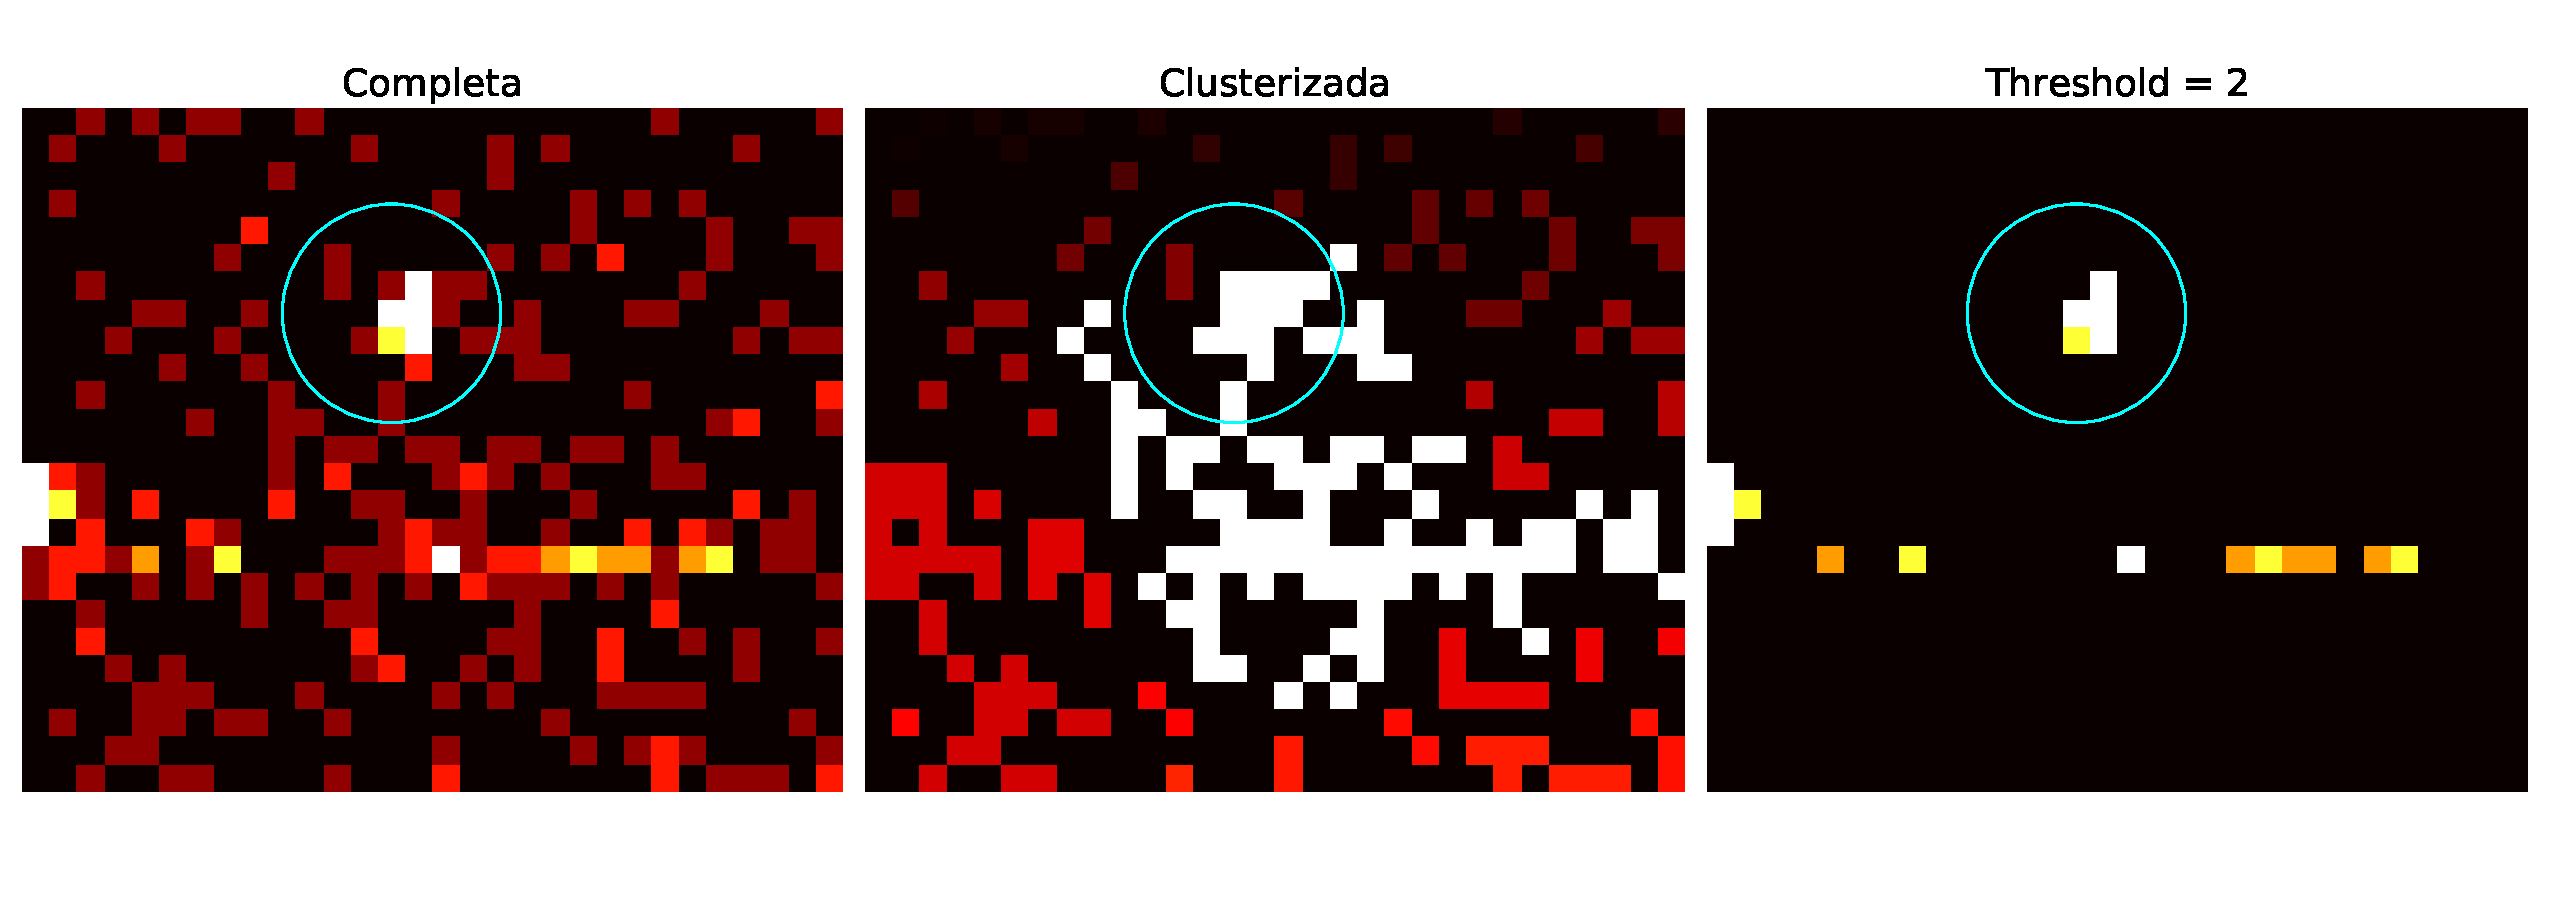
\includegraphics[scale=0.4]{Figs/despegoteo_clusters.pdf}
    \caption{\footnotesize{Ejemplo del caso de un de un evento cercano a los $180$ electrones de carga, que son los eventos de interés. En la imagen de la izquierda se ve la imagen completa, es decir, la medición sin alterar (ya convertida a unidades de carga). En la imagen del centro se en blanco y en un degrade muy tenue de rojos los diferentes clusters que el algoritmo logra reconocer. Lo importante de esta imagen es notar que el algoritmo reconoce como un unico cluster (blanco) a un número de píxeles muy grande debidido justamente a que píxeles con una unica carga generan la union entre todos ellos. Por último, la imagen de la derecha es contiene el cluster de interes una vez que los eventos de un electrón son desechados del análisis, haciendo que ahora sí se contabilice correctamente el evento de interés. Este es un evento de $174$ electrones de carga.}}
    \label{fig:ClusterPegoteado}
\end{figure}
De esta forma, se rehicieron los análisis de las imágenes con diferentes valores del corte de calidad, \verb|EPIX = 0.5|, \verb|EPIX = 1.5| y \verb|EPIX = 2.5| y se compararon los resultados obtenidos, tanto para el conteo total de eventos, como los valores finales del factor de Fano y la energía de creación electrón-hueco. Cabe aclarar que estos son resultados preliminares. Esto se hizo para $3$ de los $4$ cuadrantes del sensor, también llamados OHDU's, y se tuvo en cuenta la suma de los 3 cuadrantes funcionales.\\
\indent En las figuras \ref{fig:EntradasVsEpix}, \ref{fig:EnergiadeCreacionVsEpix} y \ref{fig:FanoVsEpix}  puede verse la variación de estos parámetros dependiendo del valor de umbral usado. El gráfico más importante en este punto es el de la figura \ref{fig:EntradasVsEpix}, donde se ve un drástico aumento en la cantidad de entradas (eventos contabilizados) cuando se varía el \verb|EPIX|. Se graficaron en cada figura las modificaciones para $3$ de los $4$ cuadrantes del sensor y para la suma de los cuadrantes $1$, $3$ y $4$. El cuadrante $2$ no funciona correctamente y por eso sus datos no han sido utilizados.
\begin{figure}[h]
%Para hacer estas figs hay que ir a /home/igna/Escritorio/Tesis2021/Figs/pys_para_plots y correr plots_entries_fano_eh.py que usa los datos que están en /home/igna/Escritorio/Tesis2021/Figs/txts_para_plots y se llaman Entries_count.txt
    \centering
    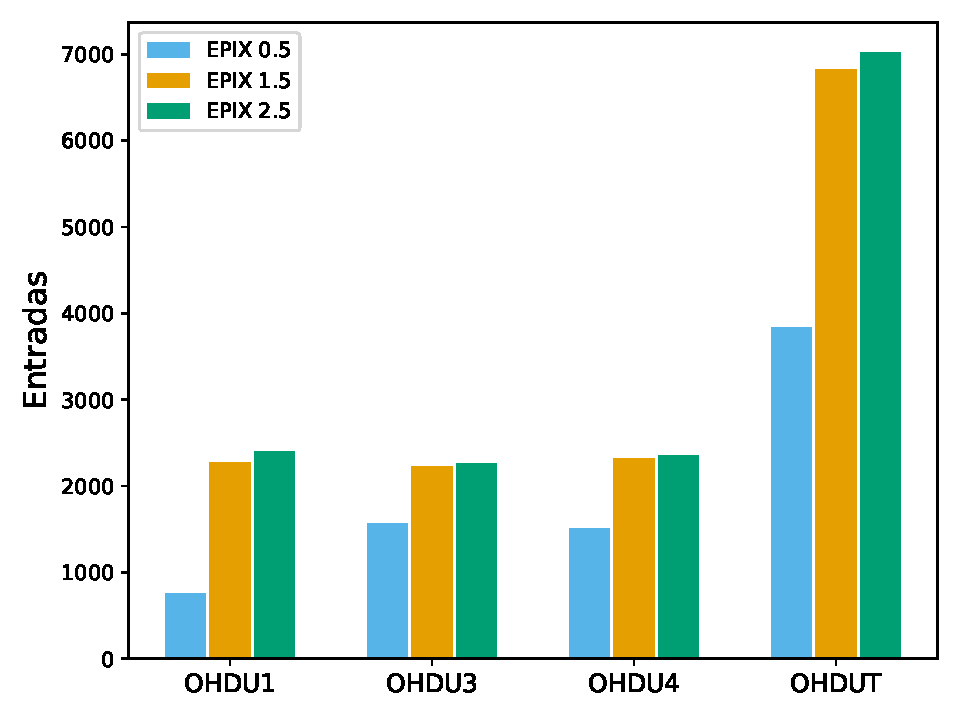
\includegraphics[scale=0.5]{Figs/Entradas_vs_Epix.pdf}
    \caption{\footnotesize{Gráfico de barras para las diferentes cantidad de entradas contabilizadas por el programa, tanto para valores diferentes de EPIX como para los diferentes cuadrantes del sensor. OHDUT hace referencia a la suma de las entradas del resto de los cuadrantes funcionales ($1$, $3$ y $4$). Se observa un aumento de más del doble en la cantidad en la cantidad de entradas para el primer cuadrante, y un aumento importante pero menos pronunciado para el resto de los cuadrantes.}}
    \label{fig:EntradasVsEpix}
\end{figure}
Se puede ver como los cuadrantes $1$, $3$ y $4$ tienen un cambio pronunciado en la cantidad de entradas al pasar de \verb|EPIX = 0.5| a \verb|EPIX = 1.5|, lo cual implica un aumento en la estadística, que era lo que se esperaba. En cambio, al pasar de \verb|EPIX = 1.5| a \verb|EPIX = 2.5| el aumento en el número de entradas es mucho menor. Particularmente, el primer cuadrante tiene un aumento muy importante en la cantidad de entradas en relación a los otros cuadrantes. Si bien el aumento sigue siendo pronunciado, para los cuadrantes $3$ y $4$ el aumento es menor. En la tabla \ref{tab:EntriesVsEpix} están los valores precisos del cambio en el número de entradas para cada cuadrante para cada valor de \verb|EPIX|. El primer cuadrante pasa de tener $760$ entradas para \verb|EPIX = 0.5| a tener $2272$ para un \verb|EPIX = 1.5|, casi el triple, es un aumento de $\sim 198\%$. En cambio, los cuadrantes $3$ y $4$ pasan de tener $1571$ y $1503$ entradas a $2229$ y $2320$, un aumento muy similar y en torno al $\sim40\%$ y $\sim50\%$ respectivamente.
\begin{table}[h]
\centering
\begin{tabular}{@{}c|c|c|c|c@{}}
\toprule
           & OHUD 1 & OHDU 3 & OHDU 4 & OHDU 1 + 3 + 4 \\ \midrule\hline
EPIX = 0.5 & 760    & 1571   & 1503   & 3834           \\
EPIX = 1.5 & 2272   & 2229   & 2320   & 6821           \\
EPIX = 2.5 & 2399   & 2261   & 2356   & 7016           \\ \bottomrule
\end{tabular}
\caption{\footnotesize{Diferentes valores para las entradas, para cada uno de los cuadrantes, para los diferentes valores de EPIX utilizados.}}
\label{tab:EntriesVsEpix}
\end{table}
Efectivamente se observa un aumento en el conteo de eventos que reconoce el programa al aumentar el valor del parámetro \verb|EPIX|. También se observa que el aumento más pronunciado es desde $0.5$ a $1.5$. El aumento promedio en el conteo de eventos es de alrededor del $100\%$.
\begin{figure}[h]
%Para hacer estas figs hay que ir a /home/igna/Escritorio/Tesis2021/Figs/pys_para_plots y correr plots_entries_fano_eh.py que usa los datos que están en /home/igna/Escritorio/Tesis2021/Figs/txts_para_plots y se llaman Entries_count.txt
    \centering
    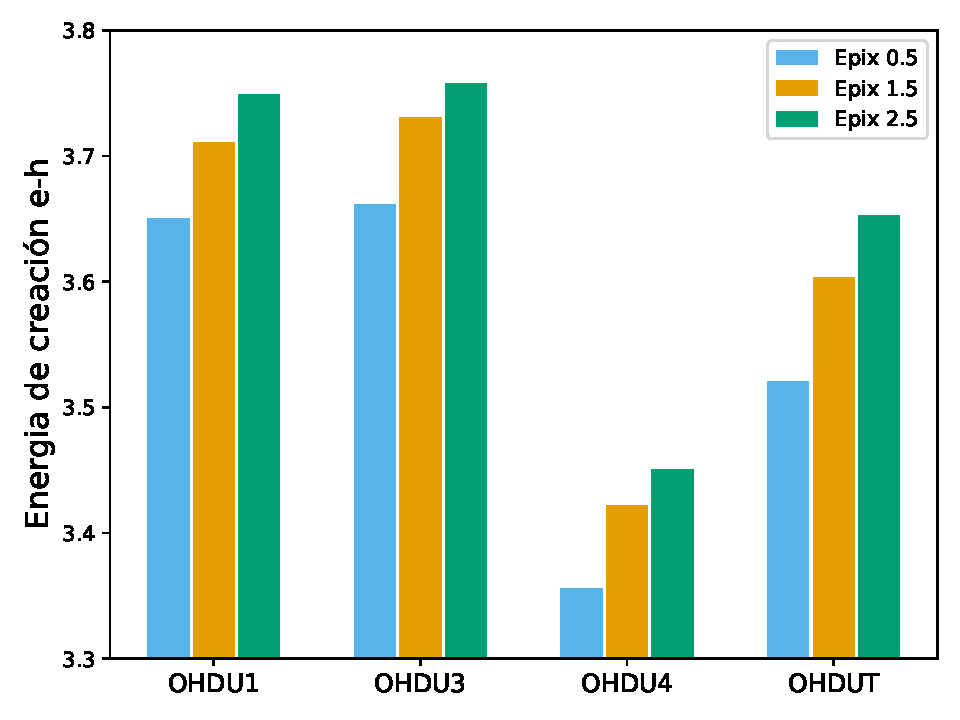
\includegraphics[scale=0.5]{Figs/EnergiaCreacion_vs_Epix.pdf}
    \caption{\footnotesize{Diferentes valores para la energía de creación electrón-hueco en función del EPIX y del cuadrante del sensor utilizado. OHDUT hace referencia a al promedio del resto de los cuadrantes funcionales ($1$, $3$ y $4$). Se observa que en todos los casos hay un aumento de la energía de creación electrón hueco cuando aumenta el EPIX.}}
    \label{fig:EnergiadeCreacionVsEpix}
\end{figure}
En cuanto al gráfico de la figura \ref{fig:EnergiadeCreacionVsEpix}, se ve como el valor preliminar para la energía de creación electrón hueco aumenta en todos los casos al aumentar el umbral \verb|EPIX|. Esto puede deberse al efecto que genera aplicar un umbral y disminuir la carga en los clusters contabilizados, que a su vez son más. Puede suceder que la cantidad de carga en los clusters sufra un corrimiento a la izquierda del valor medio real y por esto la energía de creación electrón-hueco aumente al aumentar el \verb|EPIX|: A un mismo valor de energía, una menor carga ionizada implica una mayor energía de creación electrón-hueco.
Finalmente, el caso más irregular corresponde al gráfico de la figura \ref{fig:FanoVsEpix}, donde cada cuadrante y para cada valor de \verb|EPIX| el factor de Fano dio valores diferentes y no puede definirse una tendencia a partir de estos resultados.
\begin{figure}[h]
%Para hacer estas figs hay que ir a /home/igna/Escritorio/Tesis2021/Figs/pys_para_plots y correr plots_entries_fano_eh.py que usa los datos que están en /home/igna/Escritorio/Tesis2021/Figs/txts_para_plots y se llaman Entries_count.txt
    \centering
    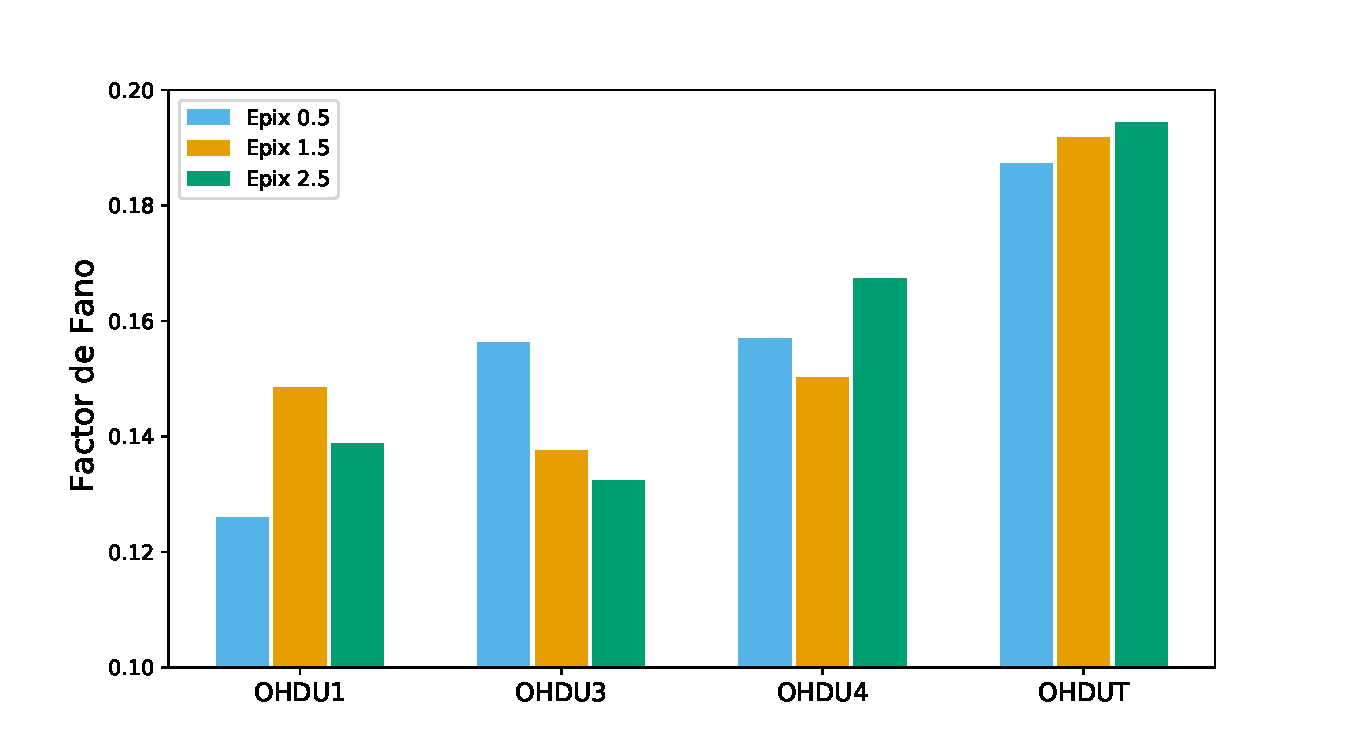
\includegraphics[scale=0.5]{Figs/Fano_vs_Epix.pdf}
    \caption{\footnotesize{Variación del factor de Fano en función del EPIX para diferentes cuadrantes del sensor. No se observa un patrón que se repita.}}
    \label{fig:FanoVsEpix}
\end{figure}
Entonces, del análisis preliminar modificando el umbral conteo de carga por píxel se puede observar el aumento deseado en la estadística para los eventos de interés de este trabajo. Como se observa que el mayor aumento en la estadística se da para \verb|EPIX = 1.5|, ese es el valor de umbral con el que se realizan los subsiguientes análisis. No está de más recordar que ese valor de umbral implica desechar los píxeles que tengan $2$ o menos electrones de carga.\\
\indent Habiendo tomado este rumbo, es necesario poder remover el sesgo producido por la eliminación de carga en los eventos medidos. Si bien definir un umbral genera un aumento en la estadística, también genera un corrimiento hacia la izquierda en los picos de interés en los espectros que debe ser corregido. Más aún, es necesario remover además el exceso de carga que tengan los clústers de interés debido a corrientes oscuras o eventos indeseados que generen un corrimiento a la derecha de los picos en los espectros. En adelante, la idea es intentar comprender el ruido de fondo en las imágenes y con ello poder corregir los valores de carga de los clústers, una vez aplicado el umbral y así mejorar la incerteza de los resultados.

%%%%%%%%%%%%%%%%%%%%%%%%%%%%%%%%%%%%%%%%%%%%%%%%%%%%%%%%%%%%%%%%%%

\chapter{Imágenes y análisis}
\section{Preliminares}
\noindent Todo el análisis cuantitativo anteriormente descripto se realizó sin la necesidad de inspeccionar visualmente las imágenes de las cuales se extraen los datos. Simplemente se aplicaron diferentes umbrales de prueba y se contabilizó el aumento en la estadística. Sin embargo, poder ver las imágenes y rápidamente poder reconocer características que se repiten, como exceso de ruido en algunas imágenes o cualquier característica que visualmente sea reconocible pero que al analizar los datos de forma automatizada pueda quedar ofuscada, es un factor importante a la hora del estudio de los datos. Dado que la cantidad de imágenes utilizadas en este trabajo es superior a las $900$, claramente observar una por una es una tarea monumental y sin sentido. Por esta razón fue necesario buscar maneras de poder extraer información contenida en todas las imágenes, de forma práctica y realizable, como por ejemplo, generar una imagen \textit{promedio} de todas las imágenes.\\
\indent Con este fin, se hizo un análisis visual, cualitativo y cuantitativo de las imágenes para comprender mejor los datos, explorar las características del sensor y de cada uno de sos cuadrantes y poder reconocer posibles deficiencias o cualquier tipo característica relevante.\\
\indent Uno de los primeros factores a caracterizar es el ruido en el sensor, donde por ruido se entiende a todos aquellos píxeles carga que no es debida eventos de ionización o eventos de interés. El ruido puede ser producto de corrientes oscuras (electrones que sufren excitaciones espontáneas debido a fluctuaciones térmicas del sensor), rebotes de un haz de baja energía en la cámara donde se encuentra el sensor y producen eventos que no son de interés en un determinado píxel, etc. No es sencillo y no existe una única manera de estimar el ruido en un sensor, por lo que en este trabajo se ensayaron deferentes maneras de encarar este análisis. \\
\indent Lo primero que se hizo en este trabajo fue buscar la manera de explorar solamente los píxeles que tuvieran una única carga. Asumiendo que en la gran mayoría de los casos, los píxeles con una única carga que se encuentran aislados de otros píxeles o de clústers de interés, son debidos a ruido del sensor, es natural empezar el análisis con estos. Una forma de caracterizar esto es tomar las imágenes y extraer todos los píxeles donde la carga sea mayor que un electrón. De este modo, se obtienen imágenes donde solo hay eventos de un electrón y todo lo demás son píxeles vacíos. En la figura \ref{fig:ImagenFitsOriginal} se puede ver una típica imagen tomada con el sensor, para el primer cuadrante, en la que claramente pueden observarse algunos eventos muy brillantes y un gran fondo. En la imagen \ref{fig:ImagenFits1e} en cambio puede verse la imagen resultante de extraer todos los píxeles cuya carga sea mayor a $1$ electrón.
\begin{figure}[h]
%Para hacer estas figs hay que ir a /home/igna/Escritorio/Tesis2021/Figs/pys_para_plots y correr imagenes_fits_original_y_filtrada.py
    \centering
    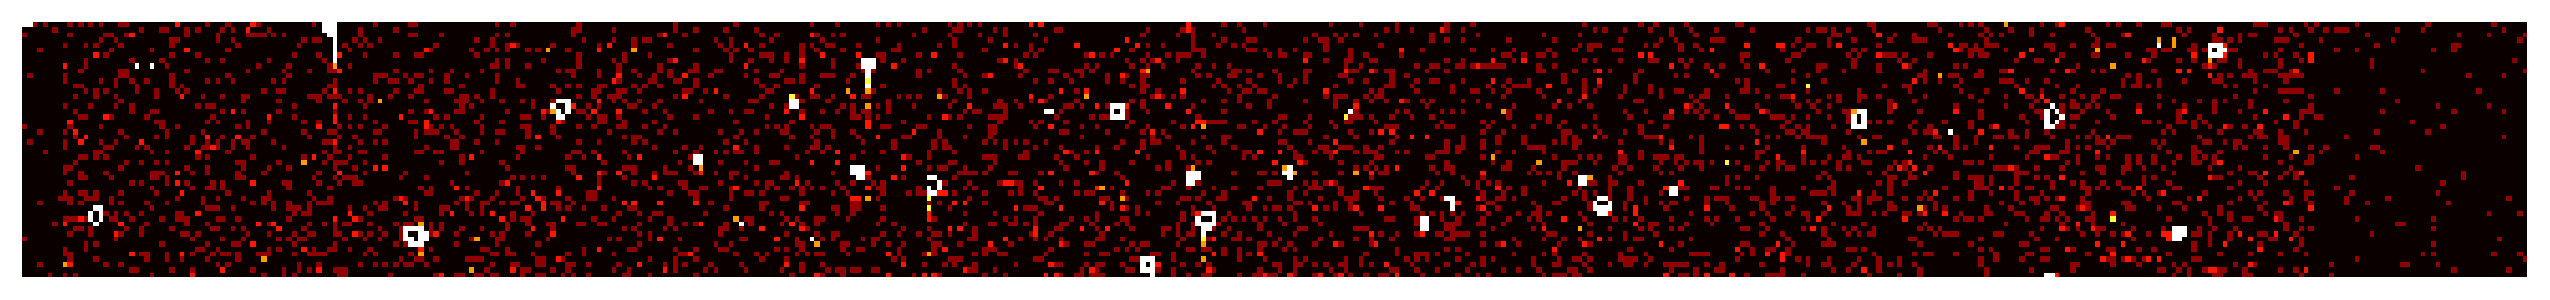
\includegraphics[scale=0.4]{Figs/imagen_fits_original.pdf}
    \caption{\footnotesize{Ejemplo de imagen tomada con el sensor, en el primer cuadrante.}}
    \label{fig:ImagenFitsOriginal}
\end{figure}

\begin{figure}[h]
%Para hacer estas figs hay que ir a /home/igna/Escritorio/Tesis2021/Figs/pys_para_plots y correr imagenes_fits_original_y_filtrada.py
    \centering
    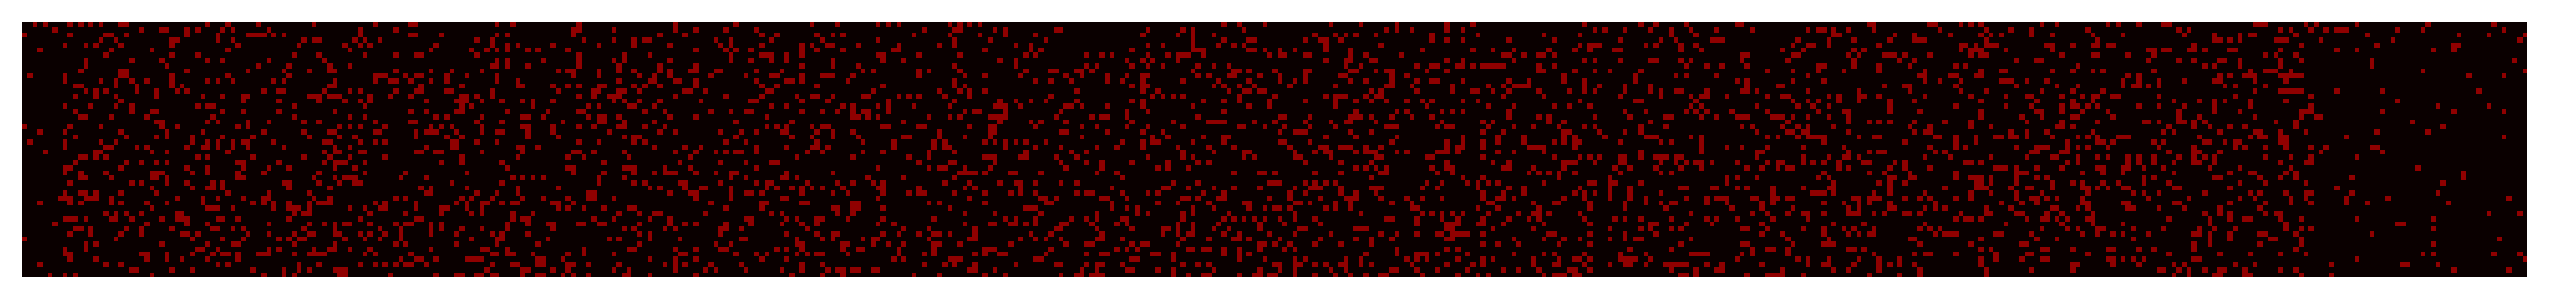
\includegraphics[scale=0.4]{Figs/imagen_fits_1_e.pdf}
    \caption{\footnotesize{Imagen resultante luego de ser extraídos los píxeles con carga mayor a $1$ electrón.}}
    \label{fig:ImagenFits1e}
\end{figure}
Una vez que se extraen los píxeles de mayor carga, se promedian todas las imágenes resultantes y se obtiene una una única imagen que condensa la información de todas las anteriores. En este contexto, promediar las imágenes implica tomar el arreglo matricial de valores ($0$ y $1$ en este caso) de carga en cada píxel (cada elemento fila y columna de la matriz) para cada imagen, y realizar la suma convencional de matrices para las $\sim 950$ imágenes. Finalmente dividir cada elemento de la matriz por la cantidad total de imágenes. De esta forma se puede ver si existen regiones con mayor o menor tendencia a concentrar este tipo de eventos.\\
\indent En la figura \ref{fig:Eventos1e} se tiene una imagen por cada cuadrante del sensor, promediados en las $925$ imágenes tomadas, donde los píxeles más brillantes son los son los que tienen mayor promedio de eventos, es decir, en el total de las imágenes esos píxeles son los que más veces tuvieron un electrón de carga. Esto también puede interpretarse como una imagen de la probabilidad por píxel de que haya un único electrón: Píxeles más brillantes son píxeles más propensos a tener carga y los píxeles más oscuros los menos propensos.\\
\indent De la figura \ref{fig:Eventos1e} pueden destacarse algunas características: Entre las que más se destacan, se encuentran:
\begin{itemize}
    \item La ausencia de carga (en promedio) en las regiones del pre-scan (región izquierda de 8 columnas de píxeles de extensión) y del over-scan (región derecha de 50 columnas de píxeles de extensión), lo cual es totalmente esperable, para todos los cuadrantes menos el segundo;
    \item El primer cuadrante es en promedio más brillante que el resto, y se observa un ligero gradiente de color entre las filas inferiores y superiores. Esto se repite, pero en menor medida en los demás cuadrantes pero no necesariamente se observa a simple vista;
    \item El segundo cuadrante (OHDU 2) capta en promedio muy poca carga. Este cuadrante del sensor es defectuoso;
    \item En los cuadrantes $3$ y $4$ se pueden ver columnas enteras de píxeles oscurecidas, que captaron muchísima menos carga (defectos del sensor?);
    \item En todos los cuadrantes (menos el segundo), se observa un único píxel (posición $x = 2$, $y = 0$) donde el promedio de carga es mucho mayor al resto. Además, la primera columna de píxeles luego del pre-scan también tiene tendencia a captar más carga que el resto;
    \item Todos los cuadrantes tienen tendencia a tener \textit{hot píxels} en el interior de la región activa, esto es píxeles aislados que tienen tendencia a captar carga más que otros, además pueden verse lineas verticales de \textit{hot píxeles} que no pueden explicarse completamente.
\end{itemize}

\begin{figure}[h]
%Para reproducir esta figura hay que ir al directorio /home/igna/Escritorio/Tesis2021/Figs/pys_para_plots y correr skipper_cuadrantes_plot.py
    \centering
    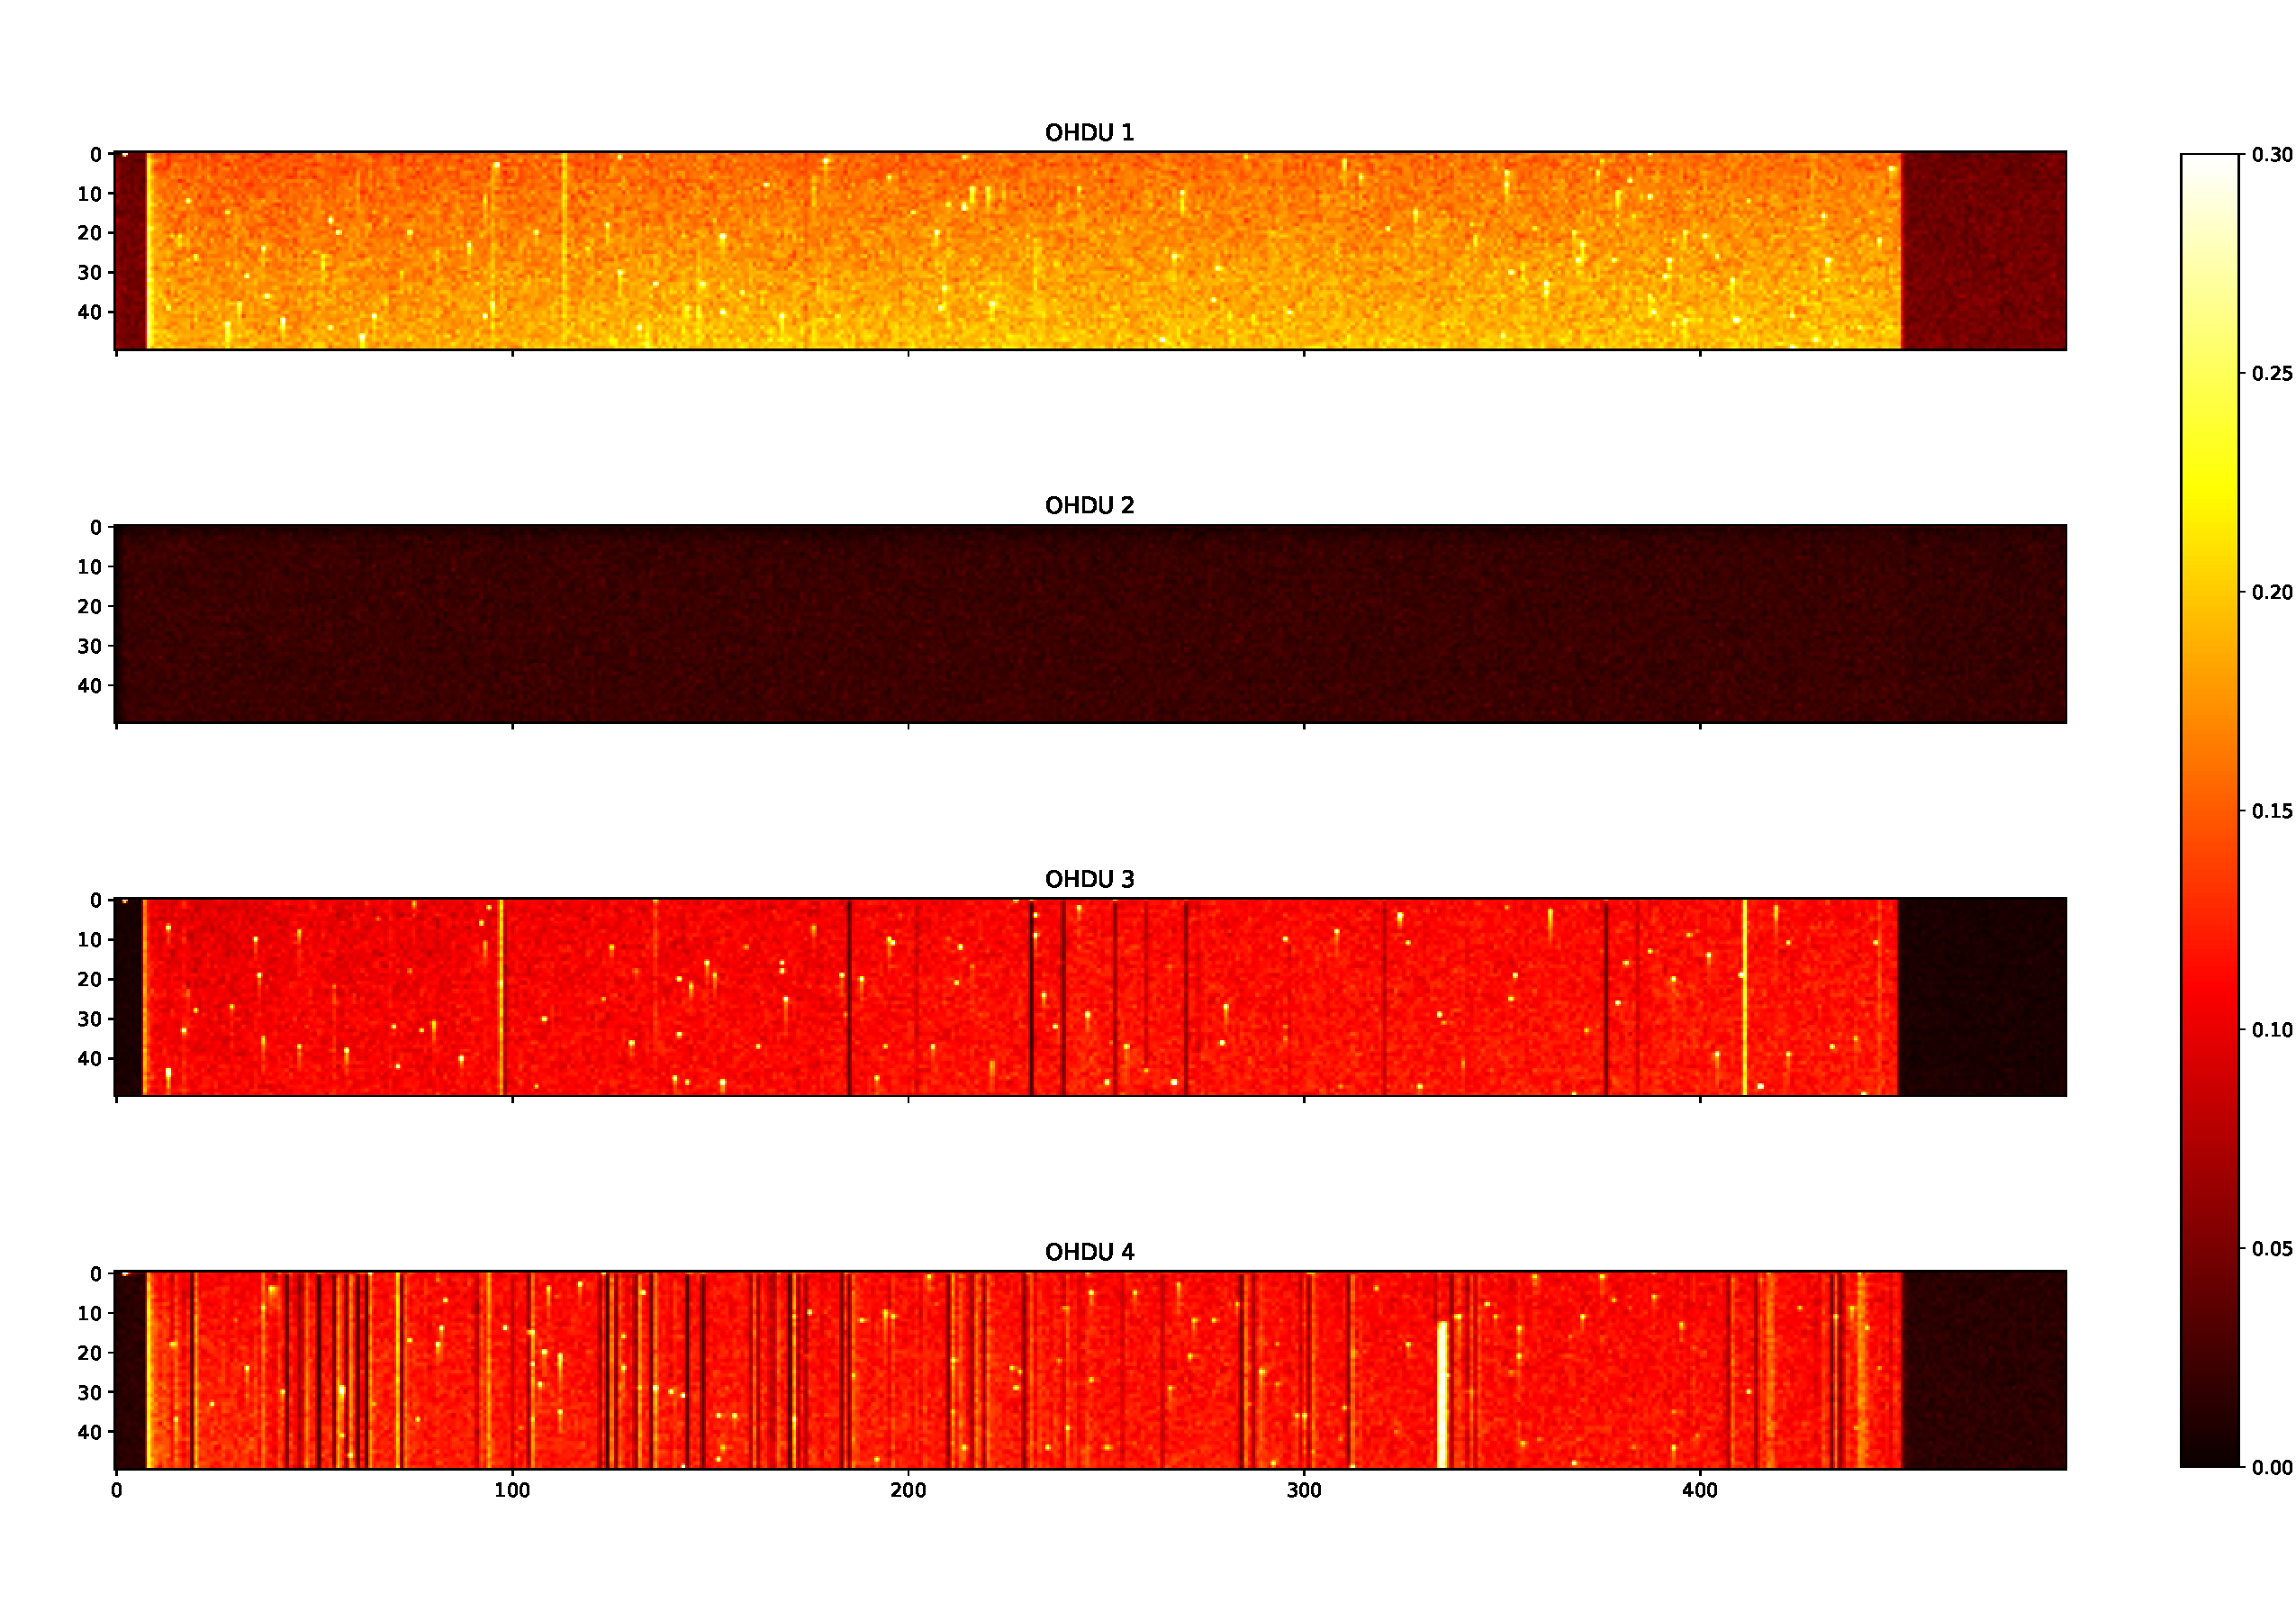
\includegraphics[scale=0.4]{Figs/1ePromedio.pdf}
    \caption{\footnotesize{Imágenes promedio para los $4$ cuadrantes del sensor. Puede verse en la escala de la derecha que los valores más altos que se obtienen rondan el $0.3$, lo cual, interpretado como una probabilidad es un $30\,\%$ de probabilidad de que en ese píxel se encuentre un evento de un electrón. En general se ve que los promedios pueden estar entre $0.1$ y $0.2$ aproximadamente. Es decir, para los cuadrantes funcionales del sensor, cada pixel tiene una probabilidad de tener un único evento que ronda entre el $10\%$ y el $20\%$.}}
    \label{fig:Eventos1e}
\end{figure}
Respecto al gradiente de color que se observa entre filas superiores e inferiores, implicaría una mayor incidencia de eventos de un electrón, en promedio, en los píxeles de las filas inferiores respecto de las filas superiores. Esto puede observarse en los gráficos de figura \ref{fig:GradienteProb}, donde se ve el aumento en \textit{la probabilidad} media por fila de que haya un evento de un electrón, a medida que el número de la fila aumenta. El gráfico de arriba a la izquierda corresponde al primer cuadrante del sensor, este es el cuadrante donde más evidente se hace este gradiente, además de ser muy lineal. La probabilidad promedio para la fila $0$ del sensor es $\sim 14.5\,\%$ y crece linealmente hasta $\sim 18\,\%$ para la fila $50$. En el gráfico de arriba a la derecha, que corresponde al segundo cuadrante, también se observa un cambio, pero solo entre las primeras 10 filas del sensor, luego la variación de la probabilidad por fila es muy pequeña y parece aproximadamente constante. Además puede ver los valores son un orden de magnitud menor a los del primer cuadrante. Para los gráficos de abajo a la izquierda y abajo a la derecha, que corresponden a los cuadrantes $3$ y $4$ del sensor respectivamente, se observan también variaciones entre las primeras filas del sensor y las últimas que parecerían tener una tendencia lineal, sin embargo, en comparación a la variación del primer cuadrante, esta es mucho menor. Por eso es difícil verlo a simple vista: La variación para el primer cuadrante es de aproximadamente del $24\,\%$ mientras que la variación de los cuadrantes $3$ y $4$ es aproximadamente del $10\,\%$.\\
\indent Esto puede deberse a que las filas superiores del sensor son las primeras a las que se les mide la carga, generando que las filas inferiores permanezcan más tiempo expuestas a fuentes de eventos. De todas maneras esta diferencia de tiempo en la lectura de las diferentes filas del sensor es muy pequeña, haciendo que estas diferencias entre filas sea pequeña, aunque apreciable en algunos casos.\\
\begin{figure}[h]
%Para modificar este plot hay que ir a /home/igna/Escritorio/Tesis2021/Figs/pys_para_plots y correr gradiente_filas_sensor.py Los datos los saca de /home/igna/Escritorio/Tesis2021/Figs/txts_para_plots y del archivo OHDU1/2/3/4_gradiente_filas_sensor.tx
    \centering
    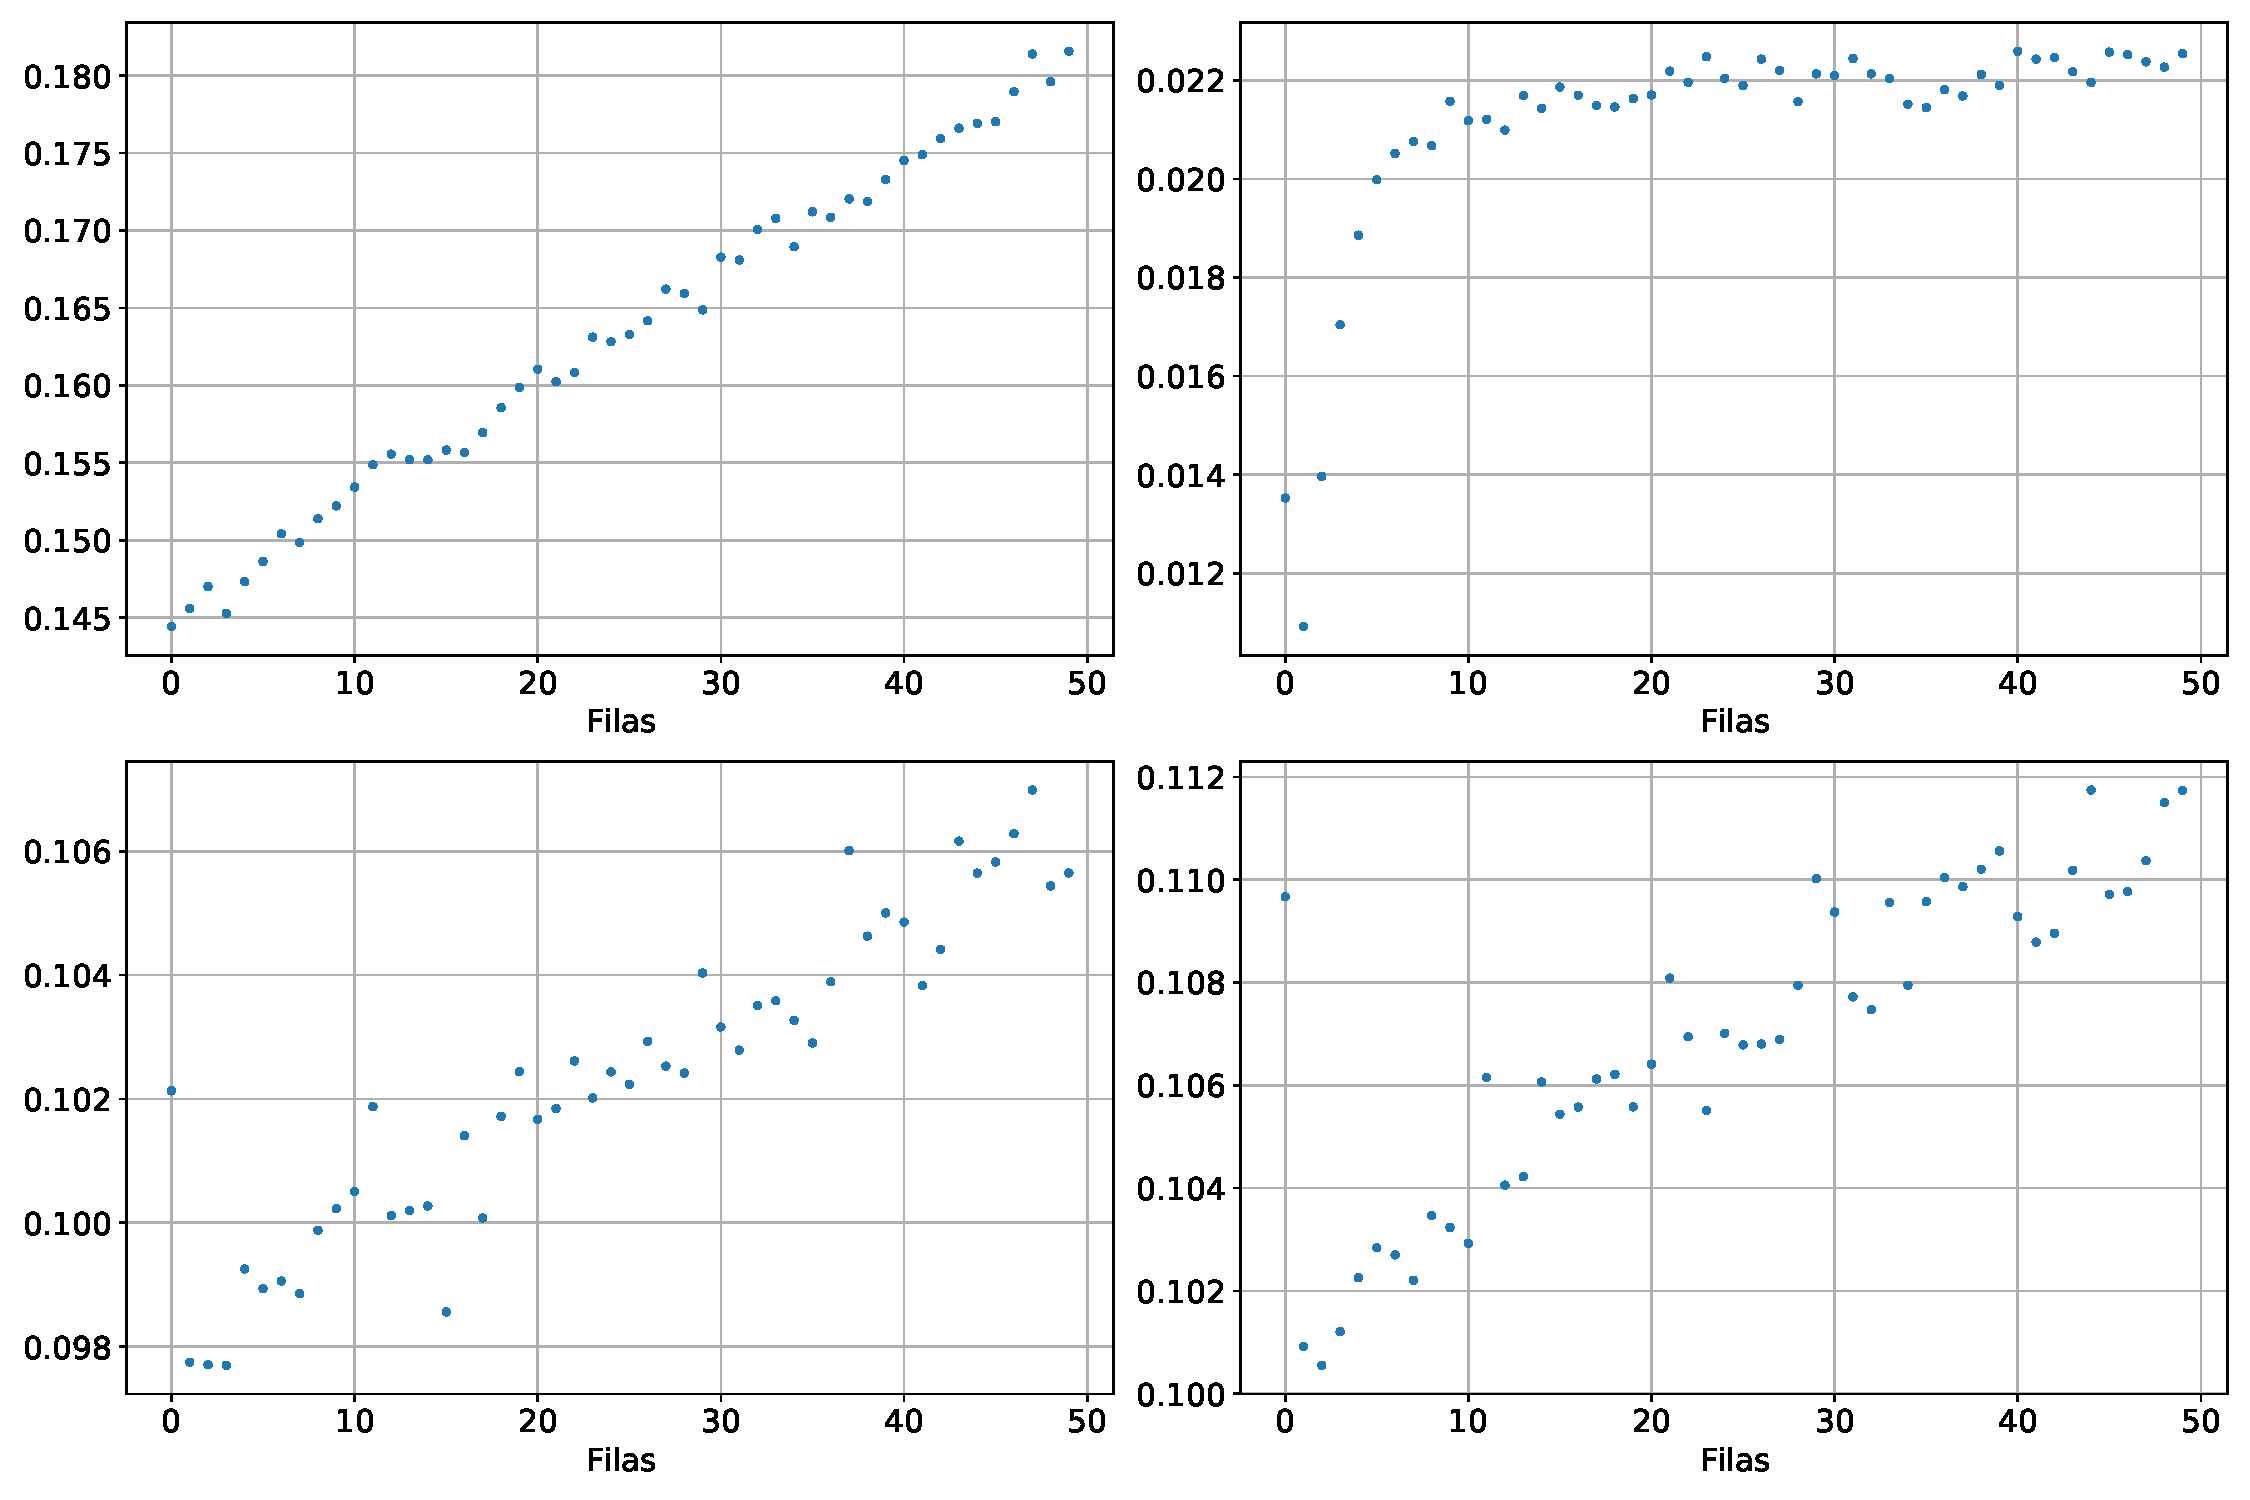
\includegraphics[scale=0.45]{Figs/Gradiente_en_filas_sensor.pdf}
    \caption{\footnotesize{Variación de la \textit{probabilidad} promedio por filas del sensor de tener un evento de $1$ electrón, para los diferentes cuadrantes. Se ven aumentos lineales de la probabilidad para los casos de los cuadrantes $1$, $3$ y $4$ y un aumento más pronunciado en relación a los demás para el primer cuadrante.}}
    \label{fig:GradienteProb}
\end{figure}
\indent Todos los análisis subsiguientes fueron realizados principalmente con el primer cuadrante del sensor, dado que es el cuadrante que funciona mejor.\\
\indent Teniendo entonces una imagen del promedio de la cantidad de eventos de un electrón, en la búsqueda por caracterizar el ruido en el sensor, lo que se hizo posteriormente fue promediar la imagen promedio de forma de obtener un promedio total y poder interpretarlo como una \textit{probabilidad} general de que en un píxel haya un evento de un electrón. Entonces, para el primer cuadrante y considerando solo la región activa del sensor, realizando este procedimiento, se obtuvo una probabilidad $p = 0.1762 \pm 0.021$, es decir, que con esta primera manera de caracterizar el ruido, hay aproximadamente un $17\,\%$ de probabilidad de que un dado píxel de la región activa del sensor tengo un electrón.\\
\indent Sin embargo, esta es una forma muy rudimentaria para intentar caracterizar el ruido del sensor, además de que no es del todo correcta. Con este camino se asume que todos los eventos de un electrón son ruido, lo cual claramente no es correcto, de forma que la probabilidad de tener un evento de un electrón en un dado píxel, calculada de esta manera, está sobrestimada. Un camino un poco más sofisticado para estimar el ruido en el sensor es explotando el hecho de que los eventos medidos en él siguen una distribución Poissoniana: bajo la suposición de que todo píxel tiene igual probabilidad de tener una carga por ruido, que dicha probabilidad es pequeña para mediciones de corto tiempo y que el número de píxeles es muy grande ($24650$ píxeles por cuadrante), entonces es esperable que la distribución que modela estos eventos sea una Poissoniana. De esta forma, si se pudiera calcular la esperanza $\mu$ de la distribución, podría saberse la probabilidad de que en un determinado píxel se encuentre un evento de un electrón o, en general, la cantidad de electrones que se deseé.\\

\section{Estimación de la esperanza de la distribución}
\noindent Si se considera una distribución Poissoniana para la variable aleatoria \textit{número de electrones por píxel}\footnote{De ruido}, se puede tomar el caso $p = P(k = 1 | \mu) = 0.1762 \pm 0.0210$, que es la probabilidad que se obtuvo previamente. De forma iterativa puede hallarse el valor de $\mu$ que satisface la expresión anterior y resulta:
\begin{equation*}
    \mu = 0.2194 \pm 0.0001
\end{equation*}
Si bien esta forma de cuantificar el ruido en los píxeles del sensor es un poco más general, dado que ahora pueden contemplarse los casos más raros, como que un píxel tenga más de una carga producto de ruido de corrientes oscuras u otros factores, este método sigue teniendo el problema de la sobrestimación de la probabilidad por píxel, al seguir asumiendo que todo píxel con un electrón es debido a ruido. Por otro lado, esta forma también presenta el inconveniente que para calcular la probabilidad hubo que hacer dos promedios, primero un promedio sobre todas las imágenes y luego un promedio sobre todos los píxeles.\\
\indent Siguiendo sobre el mismo camino, todavía bajo la hipótesis de que todo evento de un electrón es de ruido, pero evitando el cálculo de los promedios, hay una forma de calcular la esperanza de la distribución y es notando lo siguiente: Si se toman las probabilidades de que haya una sola carga por píxel y que no haya ninguna carga por píxel, es decir, se toman
\begin{equation*}
    p_{0} \equiv P(k = 0 | \mu),
    \quad
    \quad
    p_{1} \equiv P(k = 1 | \mu)
\end{equation*}
y se mira la relación entre ambas, se tiene
\begin{equation*}
    \frac{p_{1}}{p_{0}} = \frac{\mu\,e^{-\mu}}{e^{-\mu}} = \mu
\end{equation*}
y se ve que puede hallarse directamente el valor de la esperanza de la distribución. Entonces, tomando la región activa de una imagen original (sin separar los eventos de $1$ o más electrones), como la de la figura \ref{fig:ImagenFitsOriginal}, contando la cantidad de píxeles vacíos, la cantidad de píxeles con $1$ electrón y calculando la relación entre ambas, para todas las imágenes, se puede obtener directamente la esperanza $\mu$ de la distribución. De esto se obtuvo que el valor de la esperanza es :
\begin{equation*}
    \mu = 0.2245 \pm 0.0001
\end{equation*}
Los resultados de ambos métodos son parecidos, pero distintos y no se solapan sus errores. Si bien esta segunda forma para calcular la esperanza $\mu$ parece un poco más elegante y correcta, el problema sigue estando en los datos que se utilizan. El valor seguirá estando sobrestimando en tanto se considere a todo píxel con un único electrón como ruido.\\
\indent No hay que perder de vista que el objetivo de calcular la esperanza de la distribución es poder utilizarla para estimar cuánta carga extra hay sobre los clústers debida a ruido y cuánta carga no espuria fue removida debido al umbral aplicado. Conociendo la esperanza de la distribución del ruido y la cantidad de píxeles que ocupa un clúster, puede calcularse la cantidad esperada de carga extra debido a ruido que se halla en cada clúster. Teniendo estos valores, puede corregirse el valor de la carga y con eso hacer mejores estimaciones del factor de Fano y la energía de creación electrón-hueco.\\
\indent Pero también, para poder generar una corrección en el conteo de cargas por clúster y que esté lo menos sesgada posible, hay que tener en cuenta las posibles formas en las que un clúster podría tener más o menos carga. Podría suceder que sobre la superficie de los clústers hayan eventos de más, debido a corrientes oscuras u cualquier forma de ruido del sensor. Pero también, dado que en este análisis se está aplicando un umbral que elimina eventos de $2$ o menos electrones, podría suceder que a un clúster se le quiten eventos reales que se encuentran en sus bordes. Con lo cual no solo es necesario corregir la carga por exceso en los clústers, sino también por defecto.\\
\indent Con lo cual, la esperanza que se obtuvo de calcular la relación entre eventos de $1$ electrón y píxeles vacíos contiene tanto información de eventos espúrios como información de eventos genuinos. Pero lo que se persigue es poder identificar los eventos de ruido y los genuinos por separado. En ese sentido puede decirse que 
\begin{equation*}
    \mu_{T} = \mu_{bkg} + \mu_{g}
\end{equation*}
donde $\mu_{bkg}$ es la esperanza de la distribución de la variable aleatoria \textit{cantidad de eventos espurios por píxel}, mientras que $\mu_{g}$ es la esperanza de la variable aleatoria \textit{cantidad de eventos genuinos por píxel}. Hay que lograr separar ambos efectos para poder aplicar las correcciones correctamente. Queda claro que hasta el momento solo se calculó $\mu_{T}$, sin poder discriminar las contribuciones del ruido y de los eventos genuinos. La forma en la que se llevó a cabo la separación en ambas contribuciones se detalla a continuación.

\subsection{Análisis de los bordes de los clústers}
\noindent Para poder separar ambas contribuciones al calcular el $\mu_{T}$ de la distribución, la idea fue analizar los bordes de los clústers, donde ahora por clústers se entiende todo píxel individual $2$ o más electrones de carga, o conjunto de píxeles donde cada píxel tenga como mínimo $2$ electrones de carga. Es decir, se toma una imagen que tiene eventos de $2$ o más electrones, y los demás eventos se hacen $0$, como se ve en la figura \ref{fig:ImagenFits2omasElectrones}.
\begin{figure}[h]
%Para modificar este plot hay que ir a /home/igna/Escritorio/Tesis2021/Figs/pys_para_plots y correr imagen_fit_2_o_mas_e.py
    \centering
    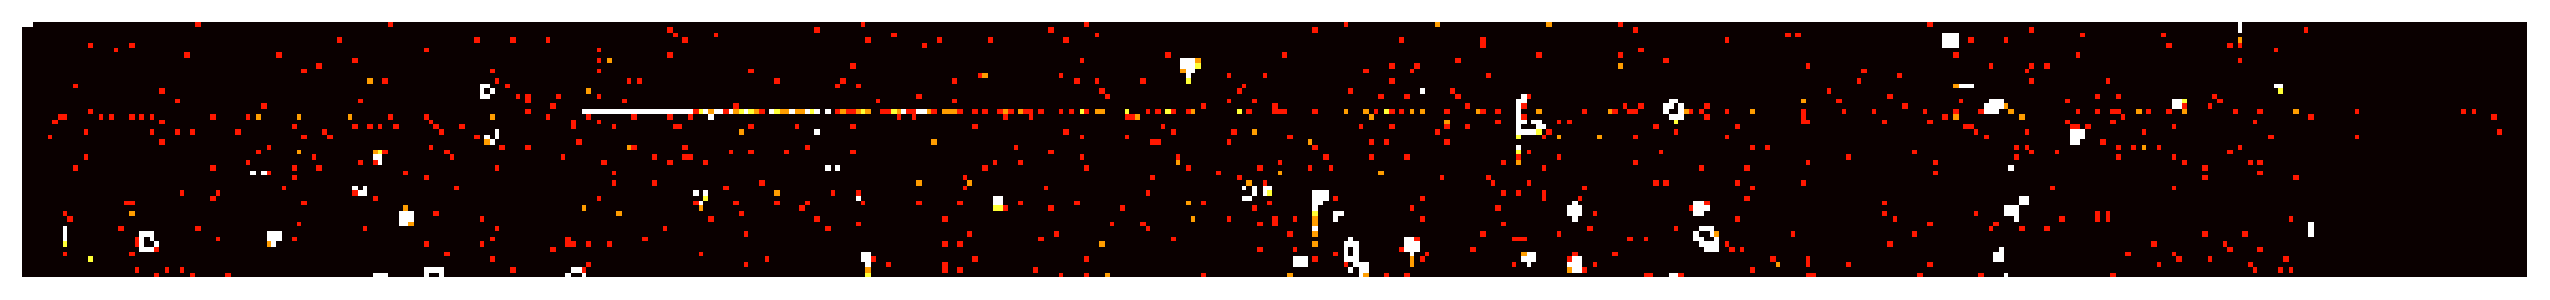
\includegraphics[scale=0.4]{Figs/imagen_fits_2_o_mas.pdf}
    \caption{\footnotesize{Imagen de ejemplo en la que solo hay píxeles que tenga más de $2$ electrones.}}
    \label{fig:ImagenFits2omasElectrones}
\end{figure}
Usando como referencia los clústers de esta imagen, se genera una máscara sobre de los bordes de estos, es decir, los píxeles inmediatamente contiguos a los píxeles con carga. Como la idea es corregir la carga en los clústers, tiene sentido mirar en el entorno de estos y no en todo el sensor.\\
\indent El procedimiento consiste en tomar los clústers y hacer una máscara de su contorno, es decir, la máscara es el conjunto de píxeles que rodea al clúster, sin incluir los píxeles cargados. Luego, superponiendo la máscara sobre la imagen original (con todos los eventos), se cuenta cuántos eventos cayeron dentro de la máscara. 
\begin{figure}[h]
%Para modificar este plot hay que ir a /home/igna/Escritorio/Tesis2021/Figs/pys_para_plots y correr imagen_bordes.py
    \centering
    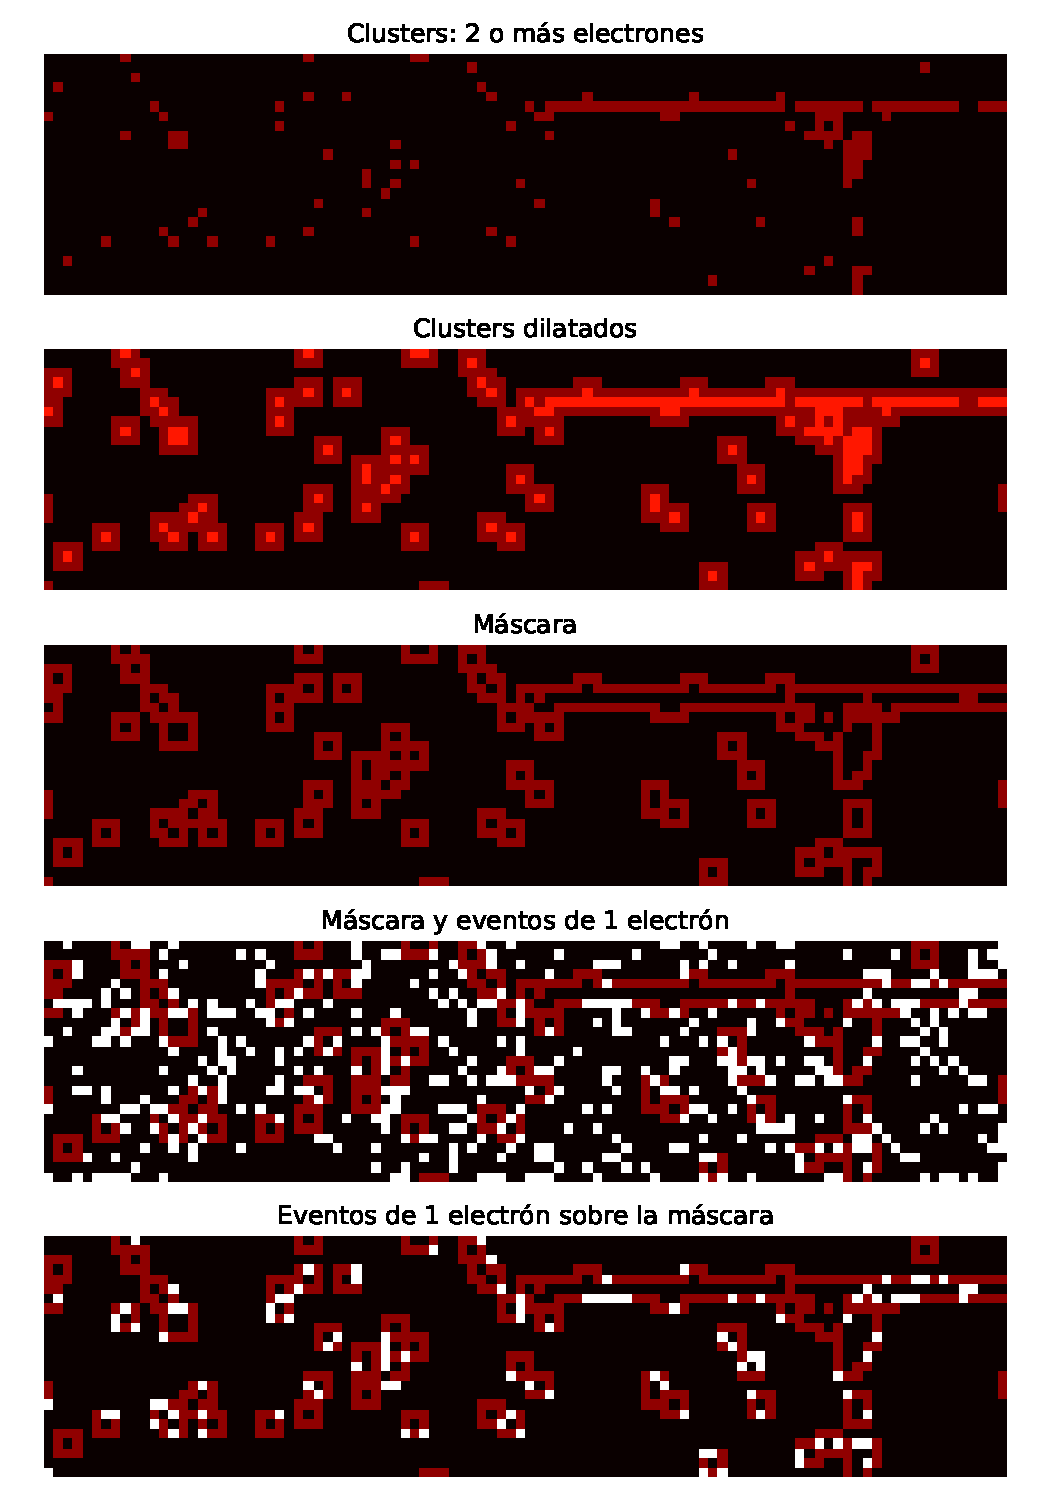
\includegraphics[scale=0.4]{Figs/analisis_bordes.pdf}
    \caption{\footnotesize{Diferentes partes del proceso de análisis de los bordes de los clusters para una imagen de ejemplo. En cada figura se ve una porción de $25 \times 25$ píxeles de área. En la primera imagen (contando de izquierda a derecha) se tiene los clústers de $2$ o más electrones. En la segunda imagen se representa la dilatación de los clústers aumentando en $1$ píxel en todas las direcciones. En la tercera imagen se ve la diferencia entre las dos primeras imágenes y se la define como la máscara a utilizar. En la cuarta se ve la máscara y superpuestos todos los eventos de $1$ electrón de esa porción del sensor. Finalmente, en la quinta se se ven solo los eventos de $1$ electrón que cayeron dentro de los píxeles de máscara. Son estos eventos los que son se cuentan en todas las imágenes, junto con los píxeles vacíos de la máscara para calcular el $\mu_{T}$.}}
    \label{fig:AnalisisBordes}
\end{figure}
Nuevamente, haciendo la relación entre eventos de un electrón y píxeles vacíos, se calcula el $\mu_{T}$. En la figura \ref{fig:AnalisisBordes} puede verse gráficamente cada uno de los pasos que se lleva a cabo para contabilizar los eventos de $1$ electrón que caen sobre la máscara. Se estima que en el borde inmediato a los clústers existe contribución de ambos efectos: eventos espurios y eventos genuinos.\\
\indent Por otro lado, para calcular la contribución de los eventos espurios, se hace el mismo procedimiento pero expandiendo los clústers en dos píxeles en todas las direcciones, y quedándose únicamente con el segundo borde, donde claramente no puede haber contribución de eventos genuinos de un cluster. Este proceso puede verse en la imagen \ref{fig:AnalisisBordesx2}. Nuevamente, de la relación entre los eventos de $1$ electrón y los píxeles vacíos, se obtiene $\mu_{bkg}$ y con este, puede despejarse el valor $\mu_{g}$.\\
\begin{figure}[h]
%Para modificar este plot hay que ir a /home/igna/Escritorio/Tesis2021/Figs/pys_para_plots y correr imagen_bordes.py
    \centering
    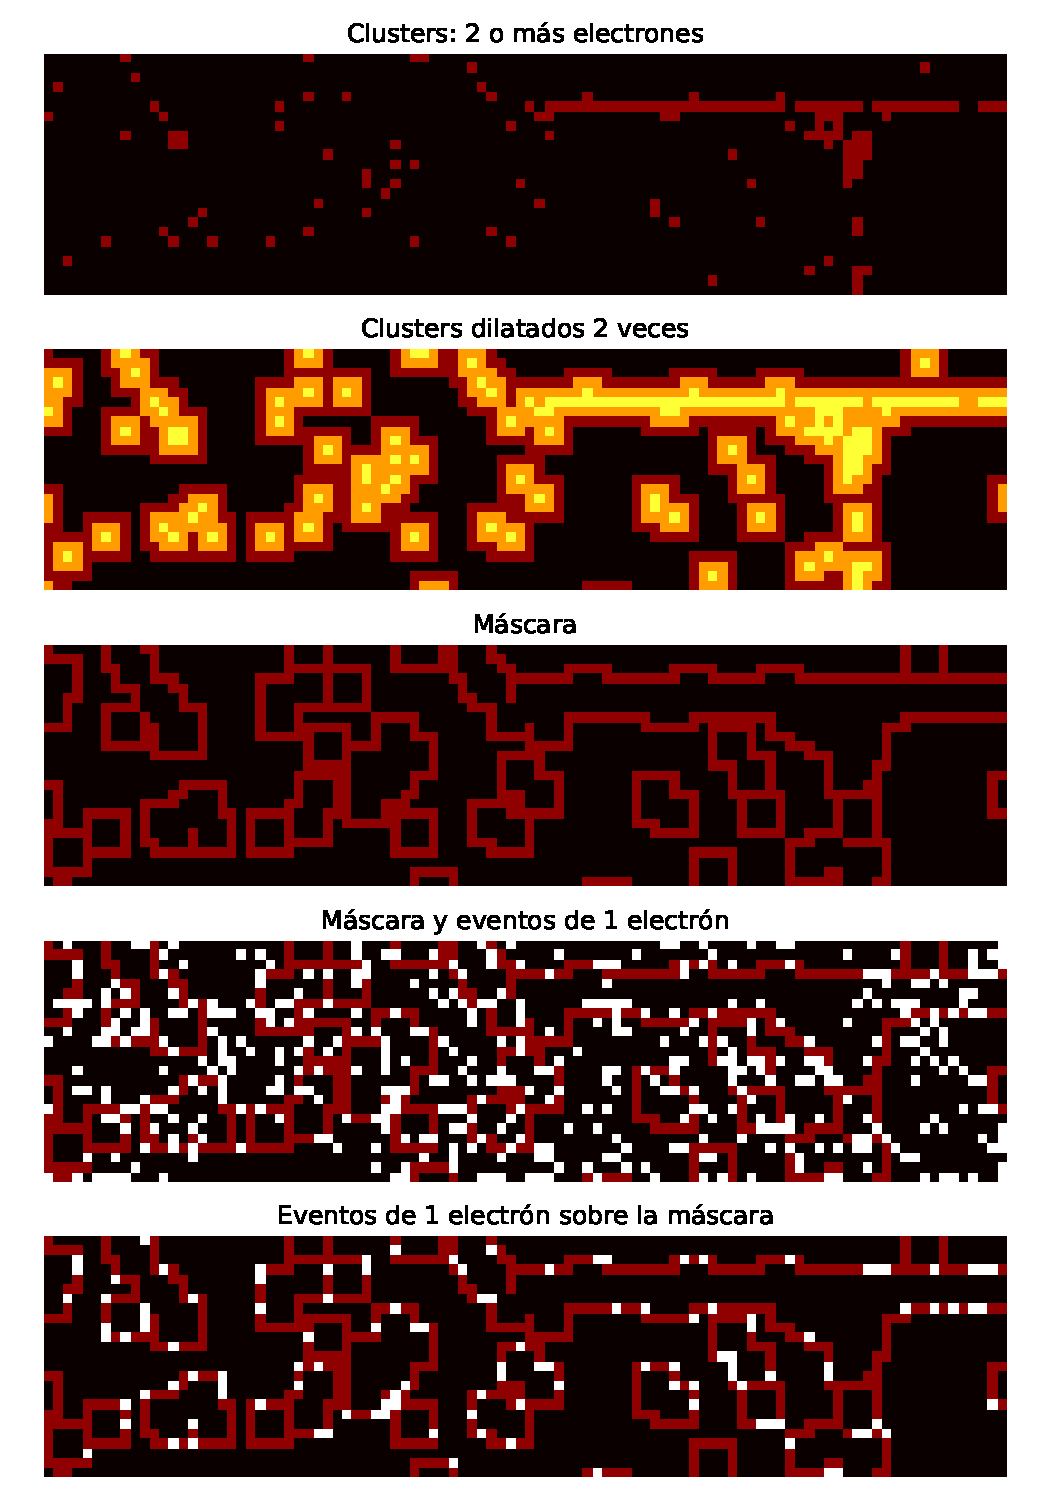
\includegraphics[scale=0.4]{Figs/analisis_bordesx2.pdf}
    \caption{\footnotesize{Análoga a la figura \ref{fig:AnalisisBordes}, pero para el caso de $2$ dilataciones, de forma de generar una máscara en el segundo borde. Los pasos son los mismos antes descriptos. De este proceso se halla la esperanza $\mu_{bkg}$.}}
    \label{fig:AnalisisBordesx2}
\end{figure}
La razón por la cual se usan los eventos inmediatamente contiguos a los bordes de los clústers para calcular el $\mu_{T}$, es porque se puede decir con seguridad que es la única región del sensor donde coexisten ambas contribuciones: $\mu_{bkg}$ y $\mu_{g}$. Tanto los eventos de un electrón que realmente pertenecen a los clústers como los eventos de un electrón que son espurios. Por otro lado, la razón por la cual se estima $\mu_{bkg}$ del siguiente cordón ($2$ píxeles de distancia al borde del clúster) se debe a que en esa zona es seguro que no pueden haber eventos genuinos de un clúster (o al menos la probabilidad de que eso suceda ronda los $10\times 10^{-14}$).\\
\indent Finalmente, de realizar estos análisis se obtuvieron los valores para las esperanzas de ambas contribuciones, que resultaron ser:
\begin{equation*}
    \mu_{T} = 0.19735 \pm 0.00024
\end{equation*} 
y el valor de la esperanza para los eventos espurios resultó 
\begin{equation*}
    \mu_{bkg} = 0.18583 \pm 0.00021
\end{equation*}
con lo cual, la esperanza para los eventos genuinos es 
\begin{equation*}
    \mu_{g} = 0.011524 \pm 0.00003
\end{equation*}
Teniendo estos valores puede corregirse el conteo de carga en los clústeres, tanto por exceso como por defecto y así tener una medición más precisa del factor de Fano y la energía de creación electrón-hueco.

\subsection{Corrección del conteo de carga}
\noindent El punto de todo el análisis anterior era poder generar las herramientas para corregir el conteo de carga que hace el programa de detección de clusters, luego de aplicar un umbral que podría eliminar carga genuina y además poder estimar cuánta carga excedente por corrientes oscuras tiene cada clúster.\\
\indent Esta corrección se llevó a cabo modificando el código del programa que con \textit{root} calcula el factor de Fano, la energía de creación electrón-hueco, y otras variables, por medio del ajuste de los espectros de carga. El programa se encarga de procesar todas las imágenes, desechar eventos que tengan carga menor a $2$ electrones (\verb|EPIX = 1.5|), filtrar eventos que no cumplan ciertos criterios (cortes de calidad), buscar los clusters, quedarse únicamente con aquellos que tengan cargas en el entorno de los $180$ electrones y calcular esos valores. Al contar la carga de estos clústers y conociendo el área de los mismos (cantidad de píxeles que los conforman), se agrega y se quita carga en función los valores hallados antes.\\
\indent Dado que la distribución de la variable aleatoria \textit{cantidad de eventos por píxel} sigue una distribución poissoniana, de esperanza $\mu$, para cada tipo evento (espurio, genuino o total) se tiene una esperanza. Para calcular la cantidad de carga que se espera que tenga un clúster de $N$ píxeles en el sensor, se puede hacer uso de las propiedades de la esperanza. Sea $Y = \sum\limits_{i = 1}^{N} X_{i}$, donde $X_{i}$ son distintas realizaciones de la variable aleatoria con distribución Poissoniana y $N$ es el número de píxeles del clúster, entonces la esperanza se calcula como
\begin{equation*}
    E(Y) = 
    E
    \left(
        \sum\limits_{i=1}^{N} X_{i}
    \right)
    = \sum\limits_{i=1}^{N}E(X_{i})
    = \sum\limits_{i=1}^{N}\mu_{i}
\end{equation*}
pero como $X_{i}$ son distintas realizaciones de la misma variable aleatoria, entonces tienen todas la misma esperanza, es decir $\mu_{i} = \mu\ \forall\ i$, con lo cual
\begin{equation*}
    E(Y) = N\mu
\end{equation*}
con lo cual, la cantidad de carga esperada para un cluster viene dada por la esperanza de la distribución, por la cantidad de píxeles. De esta forma, teniendo una esperanza total $\mu_{T} = \mu_{bgk} + \mu_{g}$, aplicando esta misma receta pueden corregirse los valores de carga por cluster. Si $n_{e}$ es la cantidad de carga medida en un dado cluster, la corrección de este valor de carga será $n_{c}$ y viene dado por
\begin{equation*}
    n_{c} = n_{e} + N\mu_{g} - N\mu_{bkg}
\end{equation*}
es decir, se agrega la cantidad de carga que se estima se pierde en los bordes por aplicar el umbral \verb|EPIX = 1.5| y se quita la carga estimada por ruido en el interior de los clústers. \textcolor{red}{Acá no me queda del todo claro como era el tema del redondeo: $N\mu_{g}$ y $N\mu_{bkg}$ claramente son float, pero la carga tiene que ser entera. El redondeo donde se hacía?}

%%%%%%%%%%%%%%%%%%%%%%%%%%%%%%%%%%%%%%%%%%%%%%%%%%%%%%%%%%%%%%%%%%

\chapter{Resultados}
Sección pendiente porque faltan los resultados.

%%%%%%%%%%%%%%%%%%%%%%%%%%%%%%%%%%%%%%%%%%%%%%%%%%%%%%%%%%%%%%%%%%

\chapter{Conclusiones}
faltan las conclusiones
    
	\pagebreak
	
	\section*{Apéndice - Simulaciones Montecarlo}
\noindent Uno de los interrogantes que se propuso responder en este trabajo es por qué el factor de Fano del sensor no vale $1$, independientemente de la energía depositada, dado que para todo proceso Poissoniano, la relación entre la varianza y la esperanza vale
\begin{equation*}
    F = \frac{\sigma^{2}}{\mu} = 1
\end{equation*} 
El factor de Fano del sensor se calcula hallando el valor medio $\mu$ y la varianza $\sigma^{2}$ de la distribución de carga correspondiente a los eventos de interés, como por ejemplo, los picos generados por los rayos $X$ del Flúor o el Aluminio. Como se sabe que el número de fotones emitidos por una fuente radioactiva sigue una distribución Poissoniana, se puede inferir que la cantidad de carga ionizada en el sensor, producto de la interacción con estos fotones, también es Poissoniana. Sin embargo, experimentalmente se observa que cuando toda la energía de la partícula incidente es depositada en el material, el factor de Fano resulta casi un orden de magnitud menor\cite{TesisKevin}. Una de las posibles razones por las que esto sucede es que la energía de los fotones incidentes no solo es disipada en forma de ionización de carga, si no también en excitación de fonones de la red cristalina del material.\\
\indent En este sentido, se buscó armar un modelo \textit{de juguete} del proceso de ionización de carga y excitación de fonones, mediante simulaciones montecarlo muy simplificadas.

\subsection*{Orden cero}
\noindent La aproximación a orden cero del mecanismo de ionización puede pensarse como una serie de experimentos de Bernoulli de éxito-fracaso, con una dada probabilidad de éxito $p$, que es la probabilidad de ionizar una carga y perder una cantidad de energía equivalente a la energía de creación electrón-hueco del Silicio, sin tener en cuenta explícitamente la disipación de energía por excitación de fonones.\\
\indent Dada una energía inicial y número fijo de experimentos de Bernoulli $N$ (que viene a modelar en cierta forma el ancho del material), puede suceder que la energía inicial se agote completamente o no, dependiendo del valor de $N$. Para una cantidad de experimentos $N$ muy grande, la probabilidad de que la energía se agote completamente es muy alta, mientras que para $N$ muy pequeño es muy probable que la energía no se pierda completamente.\\
\indent No es sorprendente que en este modelo de juguete se recupera un factor de Fano que tiende a $1$, en el caso en el que el valor de $N$ no es suficiente para agotar la energía de la partícula incidente. Y para el caso en que $N$ es tal que la gran mayoría de las veces la energía se agota completamente, el factor de Fano se vuelve menor a $1$.
\begin{figure}[H]
%Para hacer este gráfico hay que correr el script que está en esta carpeta /home/igna/Escritorio/Tesis2021/Figs/Figuras_Apendice_Simulaciones/pys_para_plots y se llama Orden0_simu_NO_atraviesa.py con los datos de esta carpeta /home/igna/Escritorio/Tesis2021/Figs/Figuras_Apendice_Simulaciones/txts_para_plots y se llama orden0_simu_NO_atraviesa.txt
    \centering
    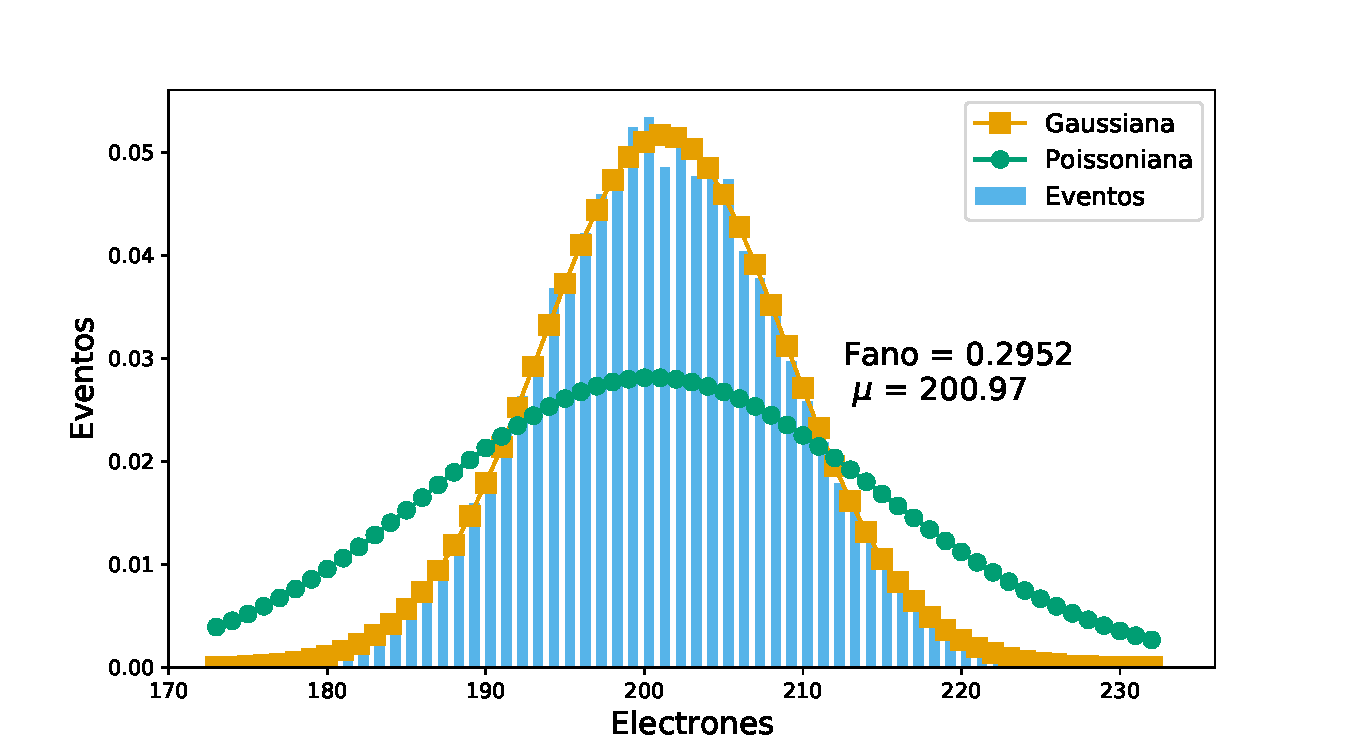
\includegraphics[scale=0.35]{Figs/Orden0_fano0.pdf}
    \caption{\footnotesize{Como reproducir esta imagen: Directorio (base) igna@Igna:~/Escritorio/Tesis2021/simulacion electrones\$ y correr ./SimuC2PyandPlot.py con parámetros: trials = 20000, distancia = 30000, atraviesa = 0 y branch git Master}}
    \label{fig:SimulacionOrden0Fano0}
\end{figure}

\begin{figure}[H]
%Para hacer este gráfico hay que correr el script que está en esta carpeta /home/igna/Escritorio/Tesis2021/Figs/Figuras_Apendice_Simulaciones/pys_para_plots y se llama Orden0_simu_SI_atraviesa.py con los datos de esta carpeta /home/igna/Escritorio/Tesis2021/Figs/Figuras_Apendice_Simulaciones/txts_para_plots y se llama orden0_simu_SI_atraviesa.txt
    \centering
    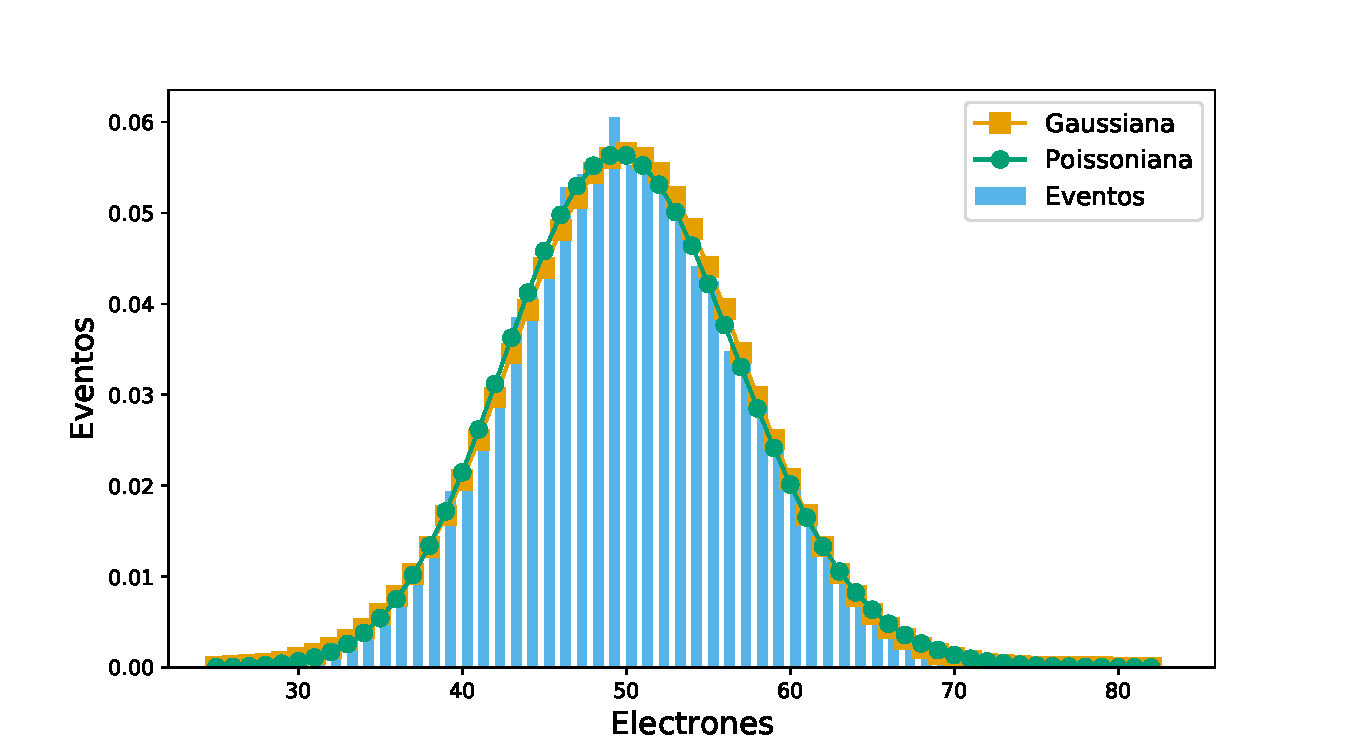
\includegraphics[scale=0.35]{Figs/Orden0_fano1.pdf}
    \caption{\footnotesize{Como reproducir esta imagen: Directorio (base) igna@Igna:~/Escritorio/Tesis2021/simulacion electrones\$ y correr ./SimuC2PyandPlot.py con parámetros: trials = 20000, distancia = 5000, atraviesa = 0 y branch git Master}}
    \label{fig:SimulacionOrden0Fano1}
\end{figure}
\noindent Si bien este modelo de juguete es una sobre-simplificación del proceso de dispersión real, los resultados de este están en concordancia con la hipótesis de que el factor de Fano es menor a $1$ debido a que la partícula incidente deposita toda su energía en el material.\\
\indent Con el fin de explorar mejor esta hipótesis, se propuso mejorar el modelo de la simulación Montecarlo. Esta vez considerando la posibilidad de que la partícula incidente pierda energía, además de por ionización, por emisión de fonones de la red. En este sentido se combinaron ideas de los trabajos de R.C. Alig et al.\cite{Alig} y K. Ramanathan \cite{Ramanathan}. En el primero proponen un modelo en el que la partícula incidente interactúa con el material, generando pares electrón-hueco por ionización en forma de cascada y, eventualmente, perdiendo energía por emisión de fonones. La forma en el que la partícula incidente va perdiendo energía depende fuertemente de la energía que tiene al momento de generar un par electrón-hueco. Esta dependencia está modelada en el segundo trabajo y lo llaman \textit{modelo simplificado}, donde proponen que la energía $E$ que se transfiere a para generar pares electrón-hueco se reparte según una distribución Beta, de la forma
\begin{equation*}
    p(x|\alpha) = \frac{2}{B(\alpha)} x^{\alpha - 1}(1-x)^{\alpha - 1}
\end{equation*}
donde $x = \frac{E}{E_{r} - E_{g}}$ es la variable aleatoria, con $E_{r}$ la energía inicial de la partícula en cada ionización, $E_{g}$ es la energía del gap del Silicio y $E$ es la fracción de energía va a parar a un nuevo par electrón hueco. Utilizando esta distribución para generar realizaciones de la variable aleatoria $x$, se puede despejar el valor de $E$ que es la energía transferida para generar pares electrón-hueco, para este modelo. Por otro lado, $B(\alpha)$ es la función Beta con un único parámetro $\alpha$, y viene dada, para el caso general por
\begin{equation*}
    B(\alpha, \beta) 
    = \frac{\Gamma(\alpha)\Gamma(\beta)}{\Gamma(\alpha) + \Gamma(\beta)}
\end{equation*}
y, para este caso particular, el parámetro $\beta = \alpha$ y $\alpha$ es el parámetro dependiente de la energía $E_{r}$ que determina el régimen de distribución de la energía, o en otras palabras, la forma de la distribución. \\
\indent La razón de la utilización de la distribución Beta para modelar como se reparte la energía en la generación de pares electrón-hueco por ionización:
\begin{itemize}
    \item \textbf{A bajas energías de la partícula incidente}, se tienen distribuciones muy picudas en los extremos posibles: $E = 0$ y $E = E_{R}+E_{g}$,
    \item \textbf{A energías mucho mayores que la energía del gap}, $E_{R} >> E_{g}$: Se tiene una distribución aproximadamente uniforme,
    \item \textbf{A energías entre $3.4\,eV$ - $4.2\,eV$ } se tiene una distribución de energía muy picuda en el medio de $x = E/(E_{R} - E_{g})$.
\end{itemize}
y estos tres casos pueden resumirse utilizando la Beta con el parámetro $\alpha$ adecuado. Para energías bajas, el parámetro $\alpha$ tiende a cero y se tiene una distribución con máximos en los extremos del intervalo. Para energías entre $3.4\,eV$ y $4.2\,eV$ se tiene una distribución con un máximo en el medio del intervalo y el parámetro $\alpha$ puede tender a infinito. Por último, para energías mucho mayores a la energía del gap, el parámetro $\alpha = 1$ y la distribución es uniforme. Estos casos se resumen el gráfico de la figura \ref{fig:BetaDist}.
\begin{figure}[H]
% Este gráfico se hace con el script que está acá: /home/igna/Escritorio/Tesis2021/Figs/Figuras_Apendice_Simulaciones/pys_para_plots DistBetaFig.py
    \centering
    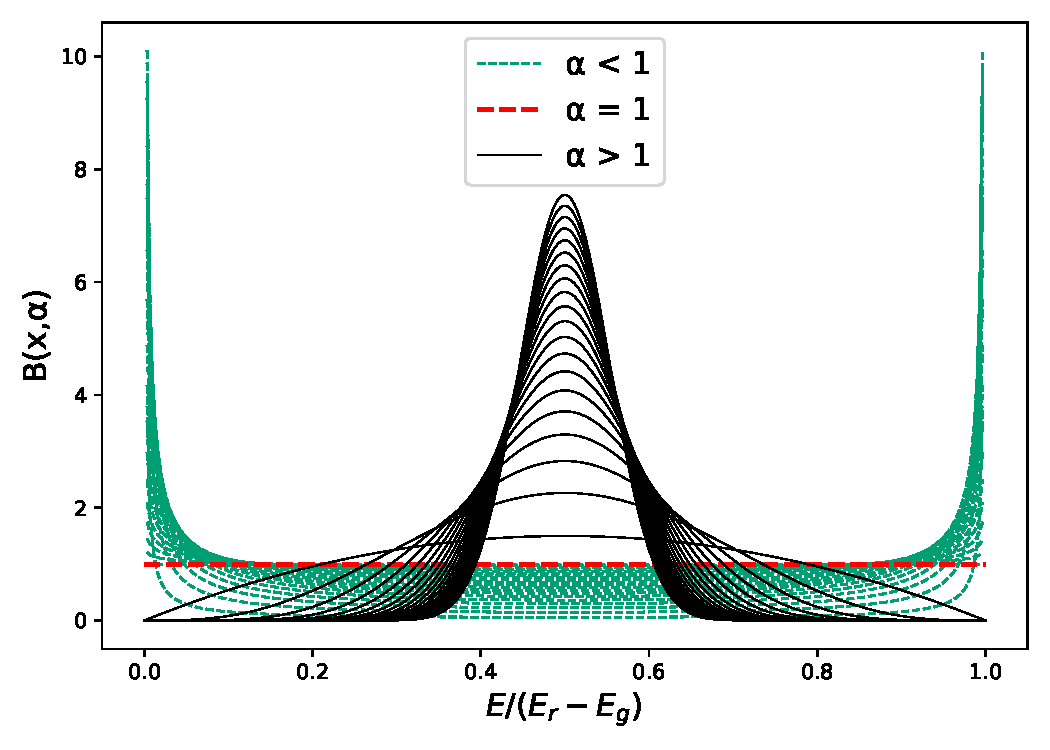
\includegraphics[scale=.7]{Figs/BetaDistFig.pdf}
    \caption{\footnotesize{Distribución Beta para diferentes valores del parámetro $\alpha$}}
    \label{fig:BetaDist}
\end{figure}

\subsection*{Orden uno}
\noindent Utilizando ideas tomadas de los trabajos anteriormente citados, se realizaron simulaciones Montecarlo para intentar reproducir el mecanismo de creación de pares electrón-hueco por ionización. Para este caso se tuvo en cuenta la posibilidad de disipación de energía por emisión de fonones, a una energía fija de $\hbar\omega_{0} = 0.063\,eV$.\\
\indent El mecanismo de cascada por el cual se producen las ionizaciones consiste en que para una dada energía inicial $E_{R}$, una fracción de esa energía se utiliza para generar un par electrón-hueco y la energía restante vuelve a fraccionarse para generar otros pares electrón-hueco. Estos pares generados, a su vez, utilizan fracciones de esa energía que les fue entregada para generar otros pares, en un proceso que se repite hasta que la energía disponible para repartir en cada rama de la cascada es menor a la energía del gap del Silicio y no es suficiente para generar más pares. Durante todo este proceso existe una probabilidad no nula de que parte de la energía se pierda por emisión fonones en la red.\\
\indent Se define una probabilidad $P_{eh}$ para la cual se produce ionización y una probabilidad $1 - P_{eh}$ para la cual se produce emisión de fonones. Esta probabilidad depende de la energía inicial, al igual que el parámetro $\alpha$ de la distribución Beta, y viene dada por
\begin{equation}
    P_{eh}(E_{R}) = 
    \left[
        1 + \frac{\Gamma_{ph}(E_{R})}{\Gamma_{eh}(E_{R})}
    \right]^{-1}
        \label{ec:ProbabilidadIonizacion}
\end{equation}
donde 
\begin{equation*}
    \frac{\Gamma_{ph}(E_{R})}{\Gamma_{eh}(E_{R})}
    = A\frac{105}{2\pi}\frac{(E_{R} - \hbar \omega_{0})^{1/2}}{(E_{R} - E_{g})^{7/2}}
\end{equation*}
con $A = 5.2\,eV^{3}$, que es una constante fenomenológica que contiene información microscópica del sistema y que además puede ajustarse para reproducir valores medidos experimentalmente. Por otro lado, $\Gamma_{ph}$ y $\Gamma_{eh}$ son las tasas de producción de fonones y pares electrón-hueco, respectivamente.\\
\indent El resultado de la simulación es simplemente el número de pares ionizados a partir de la energía inicial $E_{R}$. De esta puede verse la distribución de la cantidad de pares generados y además calcular tanto su varianza como su esperanza, para así obtener el factor de Fano.\\
\indent Otro factor a tener en cuenta en la simulación es la conservación de la energía durante el proceso de creación de pares. Puede considerarse que la energía transferida al ionizar, puede utilizarse totalmente para ionizar otros pares, o puede considerarse que siempre que se de una ionización, habrá una pequeña parte de energía que se pierde y no puede ser utilizada, es decir, que no se conserva la energía.\\
\indent Por último, en este tipo de simulación solo se puede considerar el caso en el que la partícula disipa toda su energía en el interior del material, de modo que se esperan valores para el factor de Fano menores a la unidad.

\subsubsection*{Implementación}
\noindent La implementación de los códigos que ejecutan la simulación Montecarlo se realizó con los lenguajes C y Python. Con C se realiza todo el trabajo de alto costo computacional, mientras que Python cumple un rol de interfaz para los parámetros de la simulación, como ser, por ejemplo, la energía inicial, la cantidad de corridas del Montecarlo, etc.\\
\indent A grandes rasgos, en el código en C están implementadas las funciones que hacen los cálculos antes mencionados: El cálculo de la probabilidad de ionización $P_{eh}$ a partir de la expresión \eqref{ec:ProbabilidadIonizacion}, el cálculo del parámetro $\alpha = \alpha(E_{R})$ según la energía $E_{R}$ para la distribución Beta, a partir de la cual se genera una realización de la variable aleatoria de la que se puede despejar la energía transferida a un par electrón-hueco por ionización. Finalmente, por recursión se simulan los procesos de ionización en cascada y se cuenta la cantidad final de electrones ionizados.\\
\indent Por otro lado, la función del código en Python no es más ejecutar el programa en C las veces que sean necesarias y con los parámetros iniciales de interés para obtener el resultado buscado.\\
\indent Más en detalle, el programa en C consta de un total de $6$ funciones, las cuales se listan a continuación con una breve descripción de su funcionamiento
\begin{enumerate}[label=\arabic*., listparindent=1.5em]
    \item \verb|Random()|: Es simplemente una función que genera realizaciones \verb|p_rand| de una distribución uniforme, entre $0$ y $1$. Se usa para generar una probabilidad de comparación en el Montecarlo.
    \item \verb|Peh(E_r, A)|: Es la función encargada de realizar el cómputo de la probabilidad de ionización, según la ecuación \eqref{ec:ProbabilidadIonizacion}, a partir de la energía $E_{R}$, que es un parámetro inicial que es ingresado con Python. Esta probabilidad \verb|p_eh| se compara con \verb|p_rand| en el algoritmo de aceptación del Montecarlo.
    \item \verb|alpha(E_r)|: Calcula el valor del parámetro $\alpha$ en base al valor del parámetro \verb|E_r|. Si bien el parámetro \verb|E_r| es un parámetro inicial, que para el Flúor es $677\,\si{eV}$, a medida que evoluciona el sistema, la energía se va perdiendo en ionizaciones y este parámetro es actualizado. Con cada actualización se calcula nuevamente el valor de $\alpha$ de para la distribución Beta. El valor del parámetro se calcula entonces como
    \begin{equation*}
        \alpha =
        \left\{
            \begin{matrix}
                0.1\ \mbox{si}\ E_{r} < E_{g}\\
                1\ \mbox{si}\ E_{g} < E_{r} < 2E_{g}\\
                1\ \mbox{si}\ 3.4\,\si{eV} < E_{r} < 4.2\,\si{eV}\\
                0.0207E_{r} + 0.95435\ \mbox{en otro caso.}
            \end{matrix}
        \right.
    \end{equation*}
    \item \verb|evolucionar(E_r, A, E_loss, rand_beta)|: Genera la evolución del sistema mediante Montecarlo, haciendo uso de las funciones anteriores. Implementa un bucle \verb|while|, cuya condición es que se repita el proceso mientras que la energía \verb|E_r| sea mayor que la energía del gap del Silicio \verb|E_g|. Dentro del bucle se calcula la probabilidad \verb|p_eh| de ionización, el parámetro $\alpha$, que luego es usado para generar un número pseudo aleatorio con distribución Beta del cual despejar la fracción de energía \verb|E_traf| que va a un par electrón hueco al ionizar y, por último, genera el número pseudo aleatorio de distribución uniforme con cual comparar la probabilidad de ionización en el Montecarlo.\\
    \indent Una vez que se tienen estos valores, siempre y cuando se cumpla que la probabilidad de ionizacion \verb|p_eh| sea mayor que \verb|p_rand| y que al mismo tiempo la fracción de energía \verb|E_tranf| sea mayor que $3.75\,\si{eV}$\footnote{Condición que cobra gran relevancia en los resultados y se explica en más datella en la siguiente sección} (valor medio para la energía de creación electrón hueco $\varepsilon_{\eh}$), entonces se actualiza el valor de la energía inicial \verb|E_r| restándole la fracción de energía transferida. Además, también, se guardan en una lista la resta entre las energías transferidas \verb|E_r| y la energía perdida por ionización \verb|E_loss|. Esta última es un parámetro configurable de la simulación, en la cual se puede considerar el caso donde la energía se conserva y \verb|E_loss = 0| o el caso en el que no hay conservación de energía y \verb|E_loss|$\neq$\verb|0|. Notar que la cantidad de elementos de la lista será la cantidad de pares electrón-hueco generados por una rama de la cascada con energía inicial \verb|E_r|. Luego, cada elemento de la lista se transforma, para otra rama, en \verb|E_r|, generando una nueva lista. Repitiendo con todas las energías de toda la lista y todas las sublistas, se pueden contar los electrones ionizados.\\
    \indent De no cumplirse la condición del Montecarlo, el sistema pierde energía por emisión de fonones, es decir, la energía \verb|E_r| se actualiza restándole un valor fijo de energía $\hbar \omega = 0.063\,\si{eV}$. El resultado de esta función es una lista con las energías de una sola rama de la cascada.
    \item \verb|recursion(E_r, A, E_loss, rand_beta)|: Esta función cuenta de manera recursiva la cantidad de electrones ionizados durante la cascada. La recursion, en este caso, tiene la ventaja de que es muy sencilla de implementar, pero tiene como desventaja que no es tan sencillo entender por qué funciona correctamente.\\
    \indent Lo primero que hace esta función es generar una lista energías, \verb|Energia|, llamando a la función \verb|evolucionar()| y luego se itera sobre todas estas, contando la cantidad total de elementos que posee. Esas energías son las que fueron usadas para ionizar un par electrón hueco, así que la cantidad de energías que alberga la lista es equivalente a la cantidad de pares generados. Notar que a \verb|recursion()| se le pasa como argumento \verb|E_r|. De modo que si dentro de \verb|recursion()| se vuelve a llamar a ella misma, pero ahora en vez de usar como argumento \verb|E_r|, se usa el primer elemento de la lista \verb|Energia|, es decir \verb|Energia[0]|, se produce una nueva lista a partir de una energía inicial menor y contando la cantidad de elementos. Si ahora se repite para el elemento \verb|Energia[1]|, se genera otra lista de energías. El proceso se repite hasta que todas las energías de la lista original se agotaron. Luego, las sublistas generadas repiten el proceso para todos sus elementos hasta que eventualmente la energía de las listas no es suficiente para seguir ionizando y el proceso termina.\\
    \indent El valor de salida de la función \verb|recursion()| es un entero y contabiliza la cantidad de elementos encontrados en la lista, es decir, la cantidad de electrones ionizados. Durante el proceso de recursión se van sumando todas las cantidades de carga ionizada en cada paso y finalmente se obtiene la carga total generada durante la cascada.
    \item \verb|main()|: Esta se encarga de llevar adelante las repeticiones del experimento con el fin de obtener estadística. Además, en esta se definen los parámetros necesario para la simulación, como ser la energía inicial \verb|E_r|, el parámetro \verb|A|, el valor de la energía que se pierde por ionizar \verb|E_loss|, la cantidad de experimentos que se quieren realizar \verb|trials| y la generación de un archivo \verb|.txt| con los datos obtenidos para ser levantados posteriormente con Python.
\end{enumerate}
Cabe destacar que de esta simulación el único resultado que se obtiene es la distribución de carga para una dada energía inicial $E_{r}$. Es decir, no puede conocerse ningún proceso intermedio o la \textit{historia} del proceso, solo la cantidad total de electrones generados.

\subsubsection*{Simulaciones}
\noindent Se realizaron las simulaciones partiendo de una energía inicial $E_{r} = 677\,\si{eV}$, correspondiente a los rayos $X$ de Flúor, que es el principal objeto de estudio de este trabajo. Los valores de los parámetros fueron extraídos de la bibliografía y son $A = 5.2\,\si{eV}^{3}$, la energía del gap $E_{g} = 1.1\,\si{eV}$, la energía de creación electrón-hueco promedio $\varepsilon_{eh} = 3.75\,\si{eV}$ y la energía perdida cada vez que se emiten fonones $\hbar \omega = 0.063\,\si{eV}$. El resto de los parámetros son configurables y se variaron para ver los diferentes resultados de la simulación, como ser la pérdida de energía al ionizar $E_{loss}$ y la cantidad de repeticiones del experimento \textit{trials}. La simulaciones se efectuaron con no menos de $5000$ repeticiones y con diferentes valores de $E_{loss}$.\\
\indent Se simuló el proceso de cascada con con diferente cantidad de \textit{trials}, es decir, de repeticiones del experimento, partiendo desde $5000$ hasta incluso $100000$ para asegurar la robustez de la estadística. Además, con el fin de poder caracterizar mejor las dependencias entre parámetros en la simulación, se hizo un barrido sobre la pérdida de energía $E_{loss}$ para conocer la dependencia de los resultados respecto de este, partiendo desde $0\,\si{eV}$ de pérdida de energía hasta $7\,\si{eV}$ de pérdida de energía por cada ionización (equivale a perder casi $4$ veces la energía del gap del Silicio).\\
\indent Con estos barridos se vio la dependencia de tanto del factor de Fano, como de la energía de creación electrón-hueco y del valor medio de carga ionizada al variar el valor de la energía que se pierde con cada ionización. Se observó que estos parámetros son muy sensibles a la pérdida de energía del sistema, obteniéndose resultados con cambios de regímenes muy pronunciados, particularmente, cuando la energía perdida por ionización coincide con el valor $E_{loss} = 3.75\,\si{eV}$, que casualmente es la energía de creación electrón-hueco promedio y que se usó en la simulación como un parámetro fijo en la función \verb|evolucionar()|.

\subsubsection*{Resultados}
\noindent Los resultados de las simulaciones del factor de Fano se ven en los gráficos de las figuras \ref{fig:Simulacion1rden1Fano1} y \ref{fig:Simulacion1rden1Fano2}. Ambos muestran la distribución de carga simulada, un ajuste Gaussiano a ese histograma, usando el $\mu$ y el $\sigma$ generado a partir de los datos y a su vez la forma de la Poissoniana que corresponde a ese valor medio $\mu$. Se ve claramente como la distribución de carga está lejos de parecerse a una distribución de Poisson y por ello el factor de Fano se aleja de la unidad.\\
\indent El primer caso corresponde a una simulación en la que se repitió el mismo experimento de cascada $100000$ veces para tener una buena robustez estadística, mientras que en el segundo caso se usaron $10000$ repeticiones del experimento. En la figura \ref{fig:FanoConvergencia} se observa la convergencia de los valores del factor de Fano a medida que aumenta el número de experimentos.
\begin{figure}[h]
%Este gráfico se puede hacer con el script GrafFanoConvergencia.py que esta en este directorio /home/igna/Escritorio/Tesis2021/Figs/Figuras_Apendice_Simulaciones/pys_para_plots
    \centering
    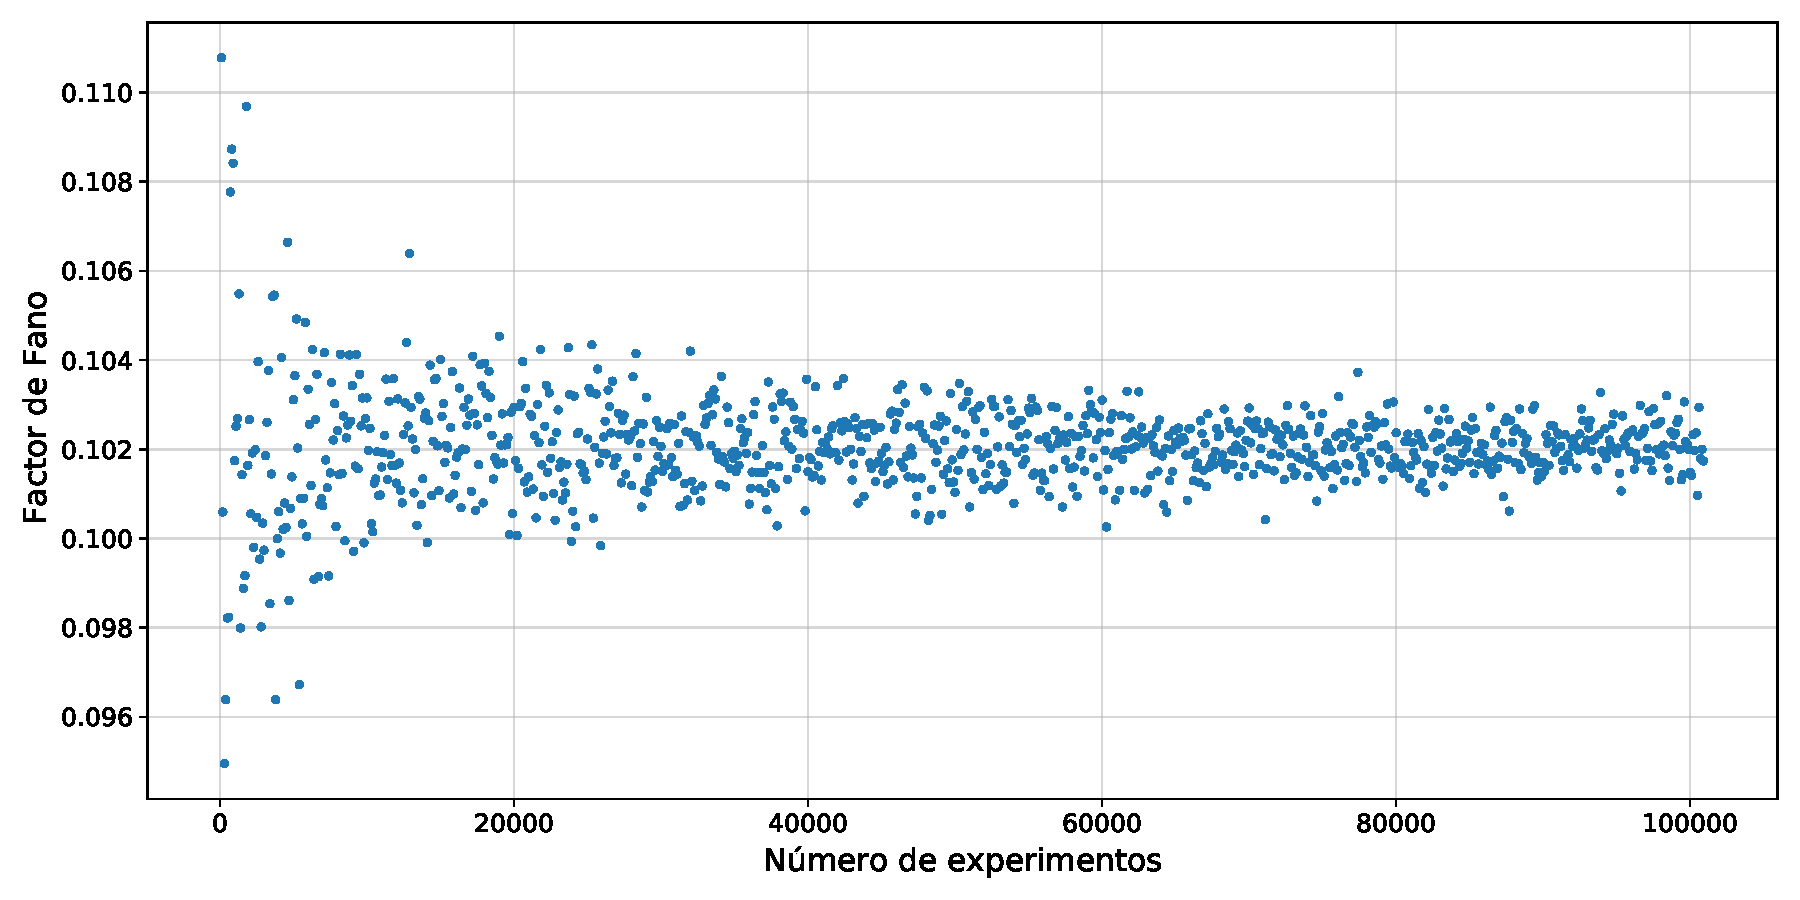
\includegraphics[scale=0.5]{Figs/FanoConvergencia.pdf}
    \caption{\footnotesize{Dispersión de los valores del Factor de Fano cada cantidad de repeticiones del experimento, partiendo desde $100$ repeticiones hasta 100900 repeticiones.}}
    \label{fig:FanoConvergencia}
\end{figure}
Para $10000$ repeticiones se ve que los valores del factor de Fano están acotados entre $\sim 0.106$ y $\sim 0.098$, mientras que para $100000$ repeticiones están acotados entre $\sim 0.104$ y $\sim 0.100$. Se nota claramente la mejora en la estadística.\\
\indent En la figura \ref{fig:Simulacion1rden1Fano1} se puede ver lo bien que se ajusta una distribución Gaussiana al histograma. En este caso el factor de Fano correspone a $F = 0.1021$ y el valor medio de carga $\mu = 192$, un valor bastante corrido a la derecha respecto del valor esperado, cercano a $\mu = 181$.
\begin{figure}[h]
%Los datos para este gráfico están en /home/igna/Escritorio/Tesis2021/Figs/Figuras_Apendice_Simulaciones/txts_para_plots Distribucion_carga_simulada_100k.txt Para modificar el graf hay que correr el .py que están en /home/igna/Escritorio/Tesis2021/Figs/Figuras_Apendice_Simulaciones/pys_para_plots Fano_100k_dist_carga.py
    \centering
    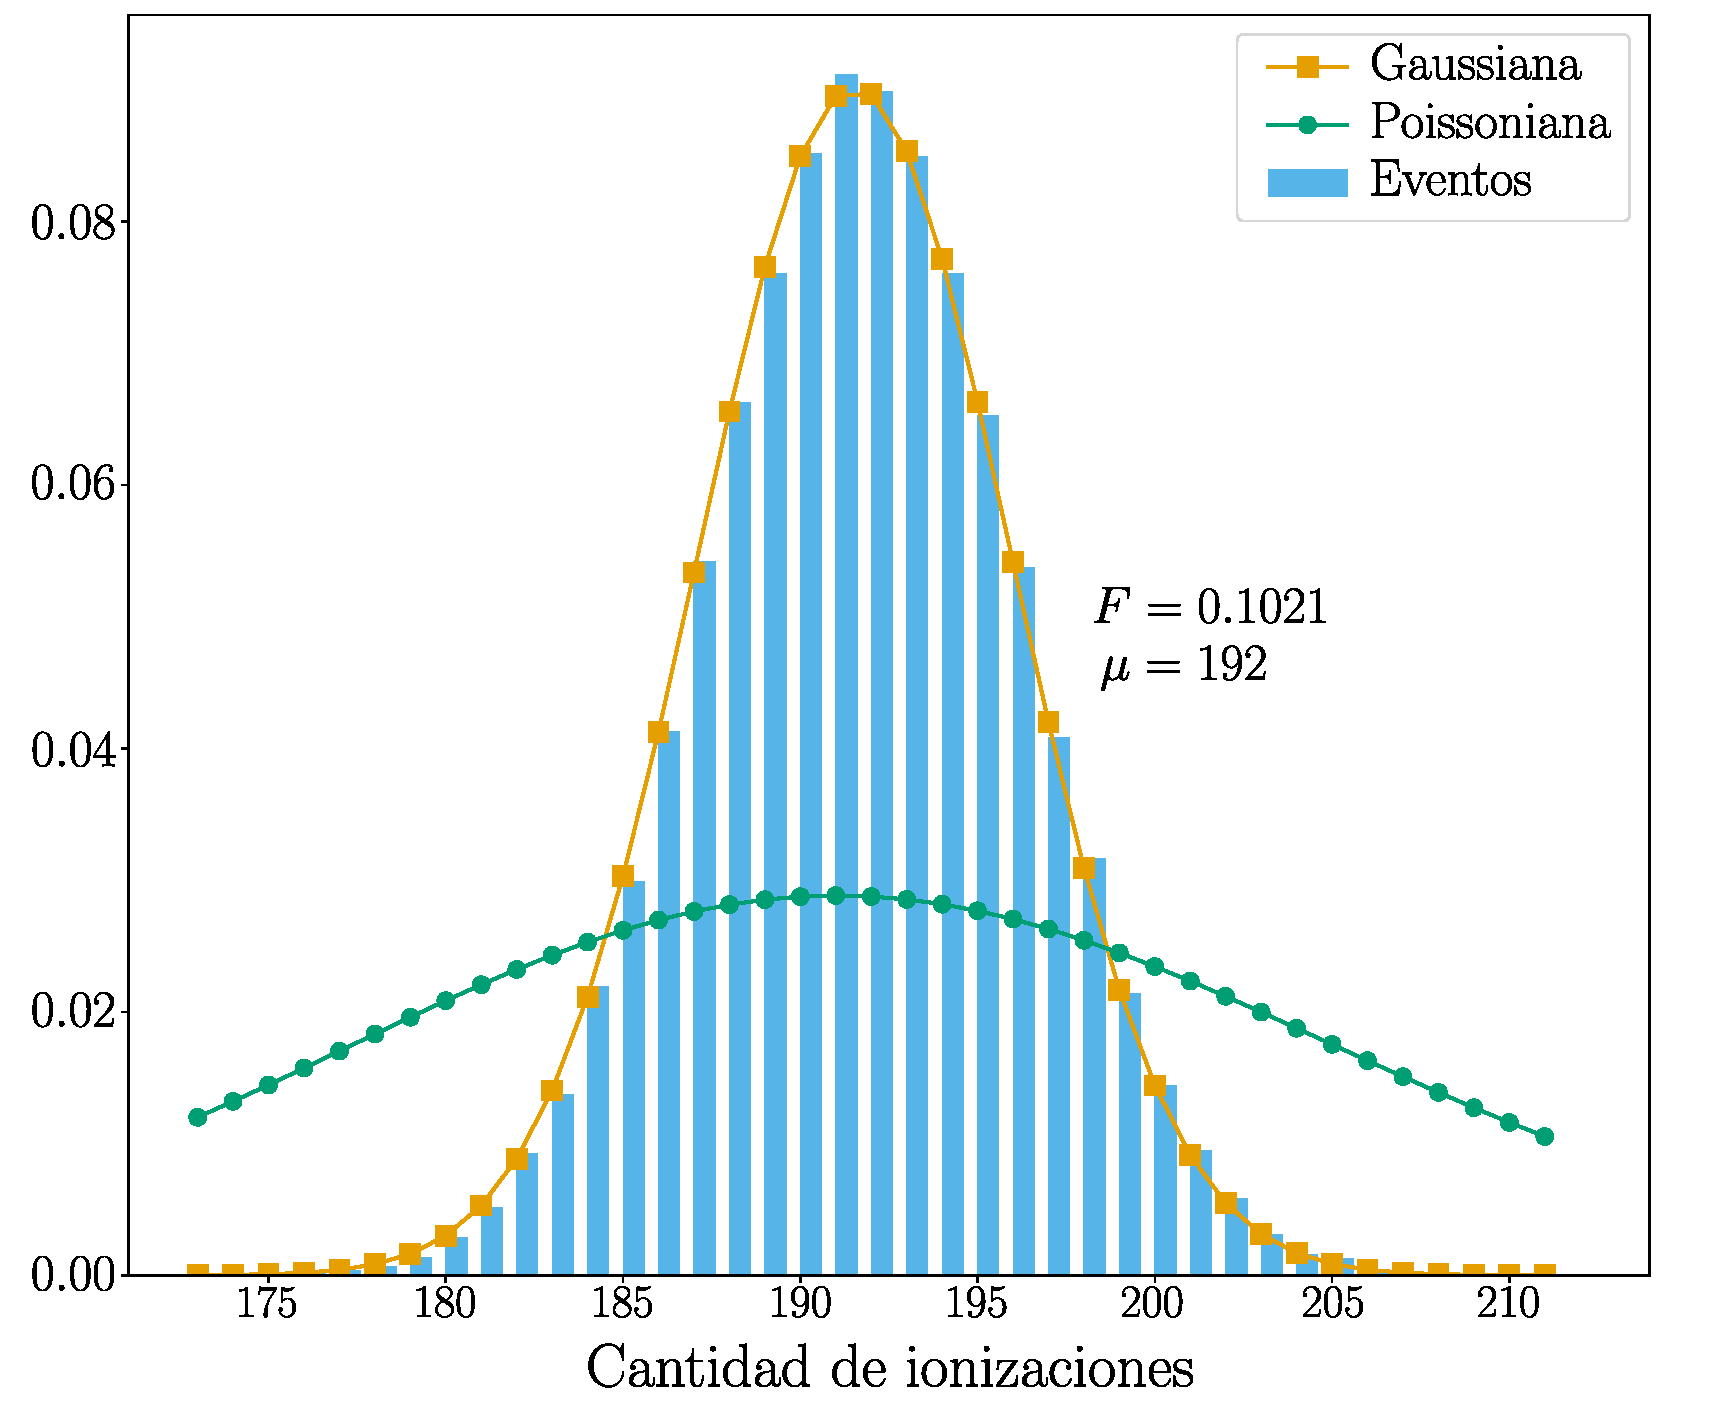
\includegraphics[scale=0.35]{Figs/Fano_677_Eloss0_100ktrials.pdf}
    \caption{\footnotesize{Distribución de carga simulada con el método de Montecarlo, con parámetro $A = 5.2\,\si{eV}^{3}$ y $100000$ \textit{trials} para obtener la mejor estadística posible. Se observa un valor medio $\mu = 192$, lo cual representa un corrimiento hacia la derecha del valor esperado para el pico de los rayos $X$ del Flúor, que es al rededor de $181$ electrones.}}
    \label{fig:Simulacion1rden1Fano1}
\end{figure}
\noindent Para el segundo caso, en la figura \ref{fig:Simulacion1rden1Fano2}, se modificó el valor del parámetro $A$ de forma que el pico coincida con lo esperado, que son $\mu = 181$ electrones. El valor de $A$ que cumple esa condición es $A = 20\,\si{eV}^{3}$, valor $5$ veces mayor al propuesto en la bibliografía para describir macroscópicamente las propiedades del Silicio.
\begin{figure}[h]
%Los datos para este gráfico están en /home/igna/Escritorio/Tesis2021/Figs/Figuras_Apendice_Simulaciones/txts_para_plots Distribucion_carga_simulada_10k.txt Para modificar el graf hay que correr el .py que están en /home/igna/Escritorio/Tesis2021/Figs/Figuras_Apendice_Simulaciones/pys_para_plots Fano_10k_dist_carga.py
    \centering
    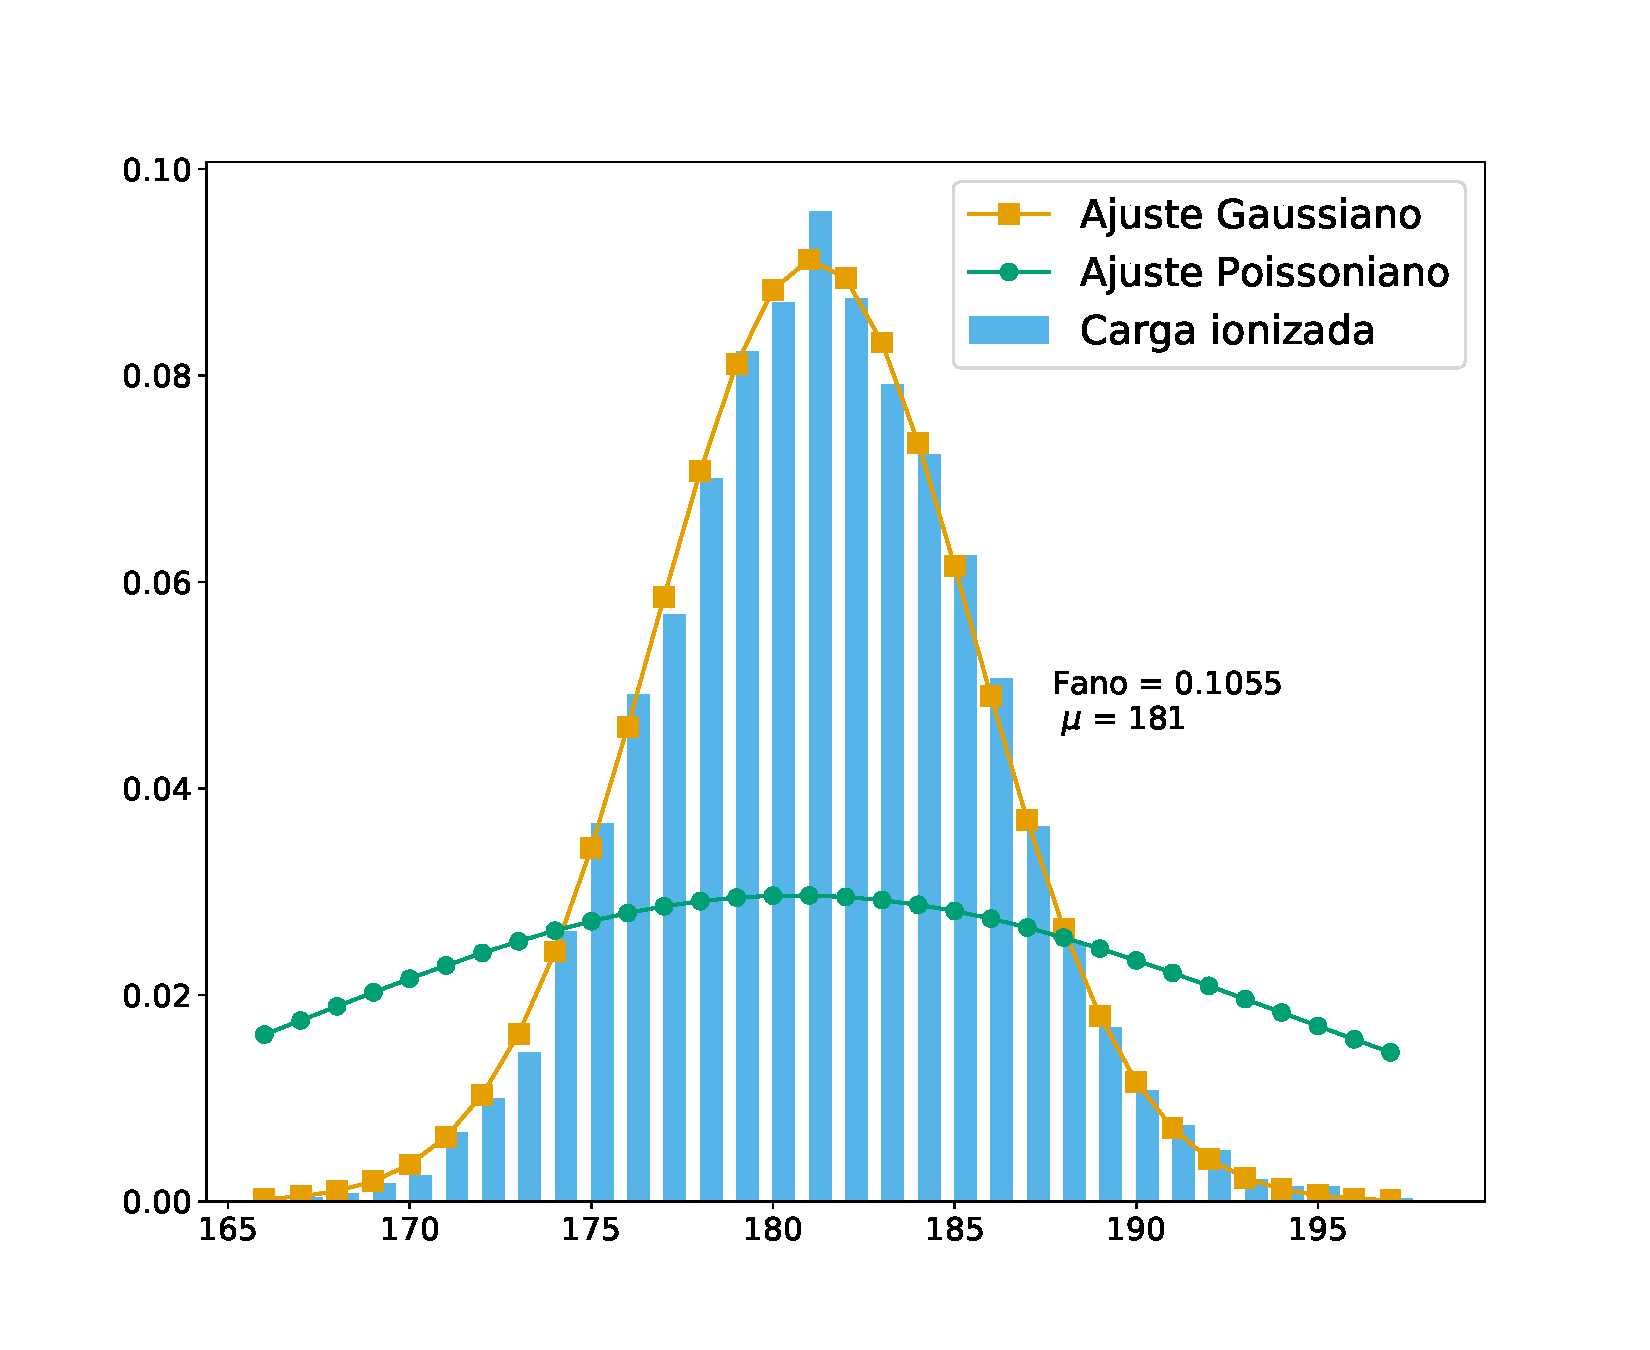
\includegraphics[scale=0.35]{Figs/Fano_677_Eloss0_10ktrials.pdf}
    \caption{\footnotesize{Distribución de carga simulada con el método de Montecarlo, forzando el parámetro $A$ para que el pico se encuentre en los $181$ electrones esperados para los $677\,\si{eV}$ de energía de los rayos X del Flúor. En este caso $A=20$ y se usaron solamente $10000$ \textit{trials}.}}
    \label{fig:Simulacion1rden1Fano2}
\end{figure}
El factor de Fano en este caso es de $F = 0.1055$, que está contenido entre las bandas esperadas para la cantidad de estadística utilizada en esta simulación. La razón por la cual usar menor estadística en este caso fue porque no era necesaria tanta robustez.\\
\indent En ambos casos el valor del factor de Fano es muy semejante y da, como se esperaba, alrededor de un orden de magnitud inferior a la unidad. Los valores esperados son << buscar valores esperados >>.\\
\indent En cuanto a los barridos, la dependencia del factor de Fano con la energía $E_{loss}$ (y al igual que la energía de creación electrón-hueco y el valor medio de carga ionizada) presenta un cambio de régimen abrupto cuando se cruza el umbral $E_{loss} = 3.75\,\si{eV}$. En la figura \ref{fig:FanoVsEloss} puede verse claramente este cambio de régimen. También se observa que cuando hay conservación de la energía, es decir, $E_{loss} = 0$, es cuando se obtiene un factor de Fano más semejante al observado experimentalmente, que está cerca de $0.1$.
\begin{figure}[h]
%a) Esta figura se puede hacer con los datos de: fano_Eloss_mu_vec.txt que está en el directorio /home/igna/Escritorio/Tesis2021/Figs/Figuras_Apendice_Simulaciones/txts_para_plots usando el .py Barridos_mu_Eloss_fano.py que está en /home/igna/Escritorio/Tesis2021/Figs/Figuras_Apendice_Simulaciones/pys_para_plots
    \centering
    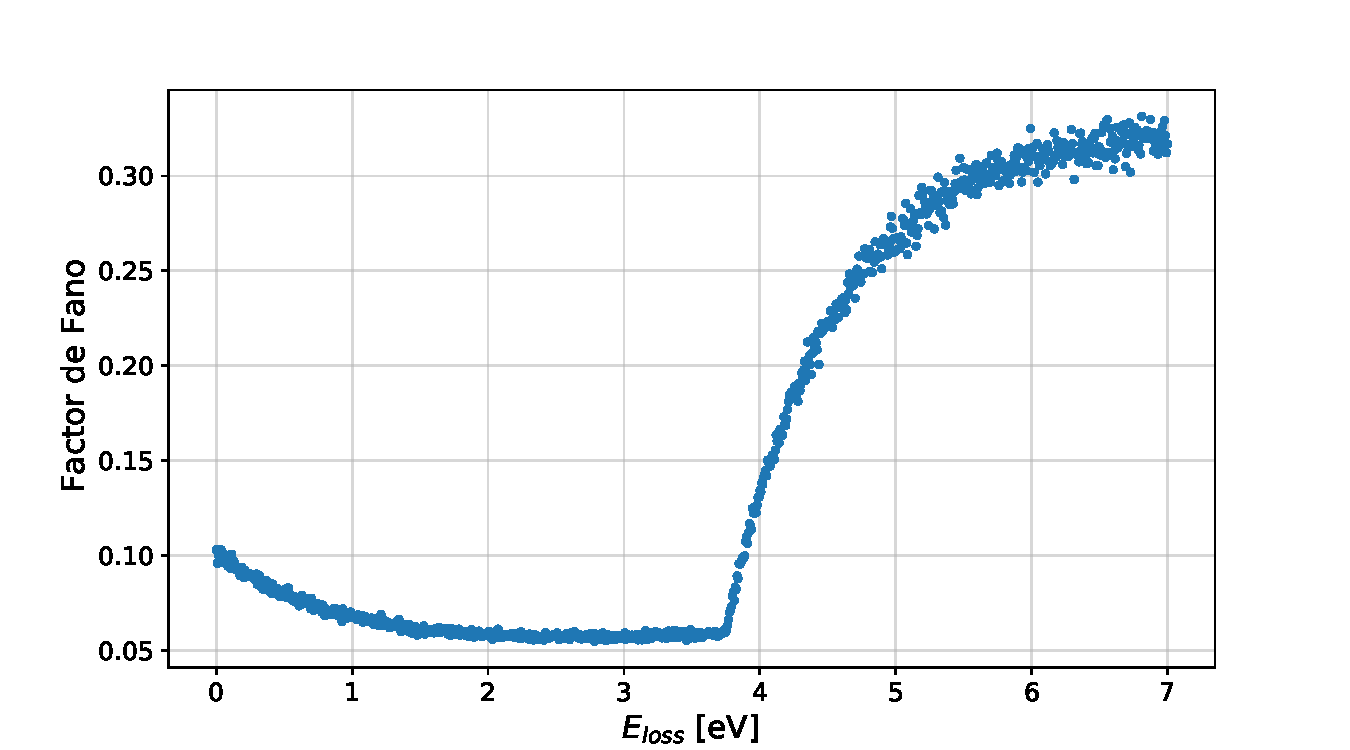
\includegraphics[scale=0.35]{Figs/Fano_vs_Eloss_5ktrials_0-7Eloss.pdf}
    \caption{\footnotesize{asd.}}
    \label{fig:FanoVsEloss}
\end{figure}
A medida que aumenta la pérdida de energía, el factor de Fano comienza a decrecer hasta que se alcanza los $3.75\,\si{eV}$ de pérdida de energía, donde se observa el cambio brusco en la curva, y se observa un aumento pronunciado de la misma, muy semejante a un punto crítico.\\
\indent De la misma forma, el valor media de la carga ionizada $\mu$ tiene un cambio de concavidad en la curva a medida que aumenta la cantidad de energía perdida por cada ionización, como se ve en la figura \ref{fig:ElossVsMu}
% b) Esta figura se puede hacer con los datos de: fano_Eloss_mu_vec.txt que está en el directorio /home/igna/Escritorio/Tesis2021/Figs/Figuras_Apendice_Simulaciones/txts_para_plots usando el .py Barridos_mu_Eloss_fano.py que está en /home/igna/Escritorio/Tesis2021/Figs/Figuras_Apendice_Simulaciones/pys_para_plots
\begin{figure}[h]
    \centering
    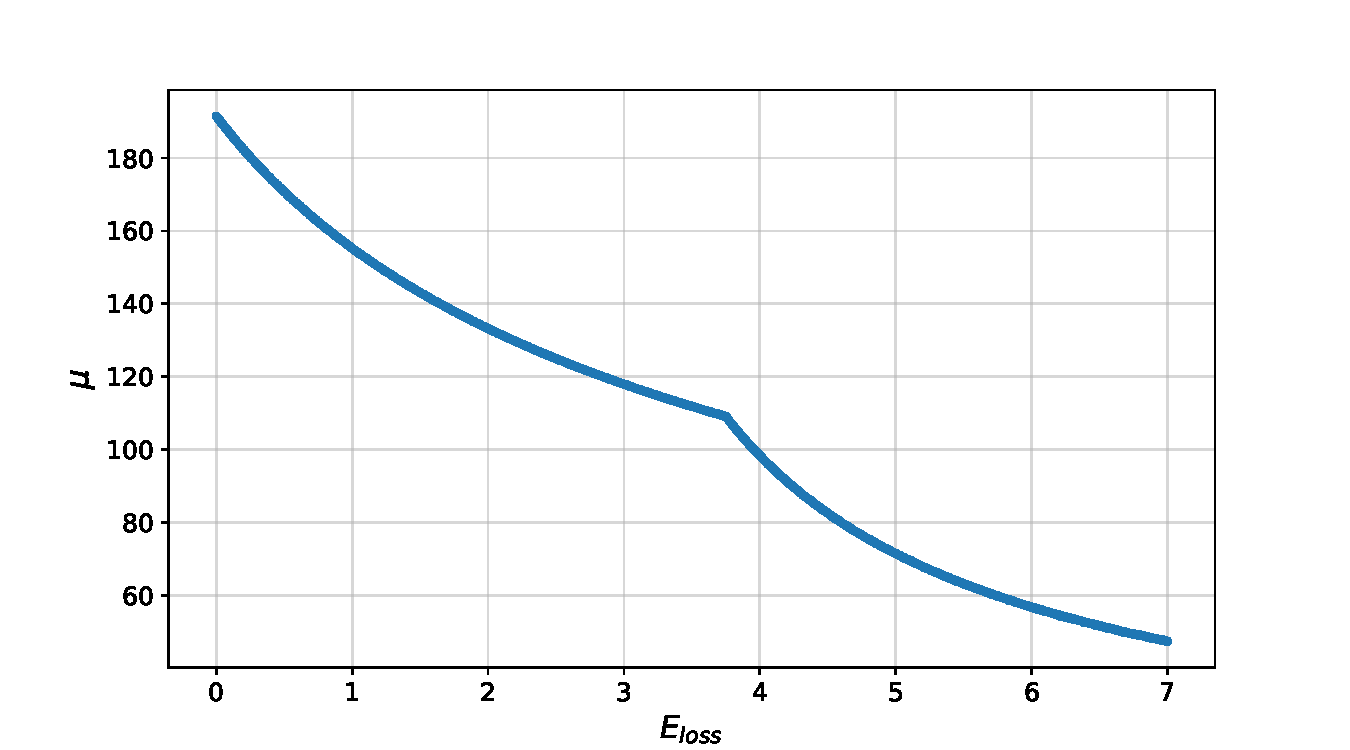
\includegraphics[scale=0.35]{Figs/ELoss_vs_mu_5ktrials_0-7Eloss.pdf}
    \caption{\footnotesize{asd.}}
    \label{fig:ElossVsMu}
\end{figure}
Nuevamente, los valores más cercanos a los medidos experimentalmente son los que corresponden a los casos en los que hay conservación de la energía.\\
\indent Por último, para la energía de creación electrón hueco, calculada a partir del valor medio de carga ionizada y la energía inicial $E_{R} = 677\,\si{eV}$, usando $\left\langle\varepsilon_{\eh} \right\rangle= 677\,\si{eV}/\mu$, claramente tendrá el mismo cambio de régimen en $3.75\,\si{eV}$, como se ve en la figura \ref{fig:CreacionHuecoVsEloss}
\begin{figure}[h]
%a) Esta figura se puede hacer con los datos de: fano_Eloss_mu_vec.txt que está en el directorio /home/igna/Escritorio/Tesis2021/Figs/Figuras_Apendice_Simulaciones/txts_para_plots usando el .py Barridos_mu_Eloss_fano.py que está en /home/igna/Escritorio/Tesis2021/Figs/Figuras_Apendice_Simulaciones/pys_para_plots
    \centering
    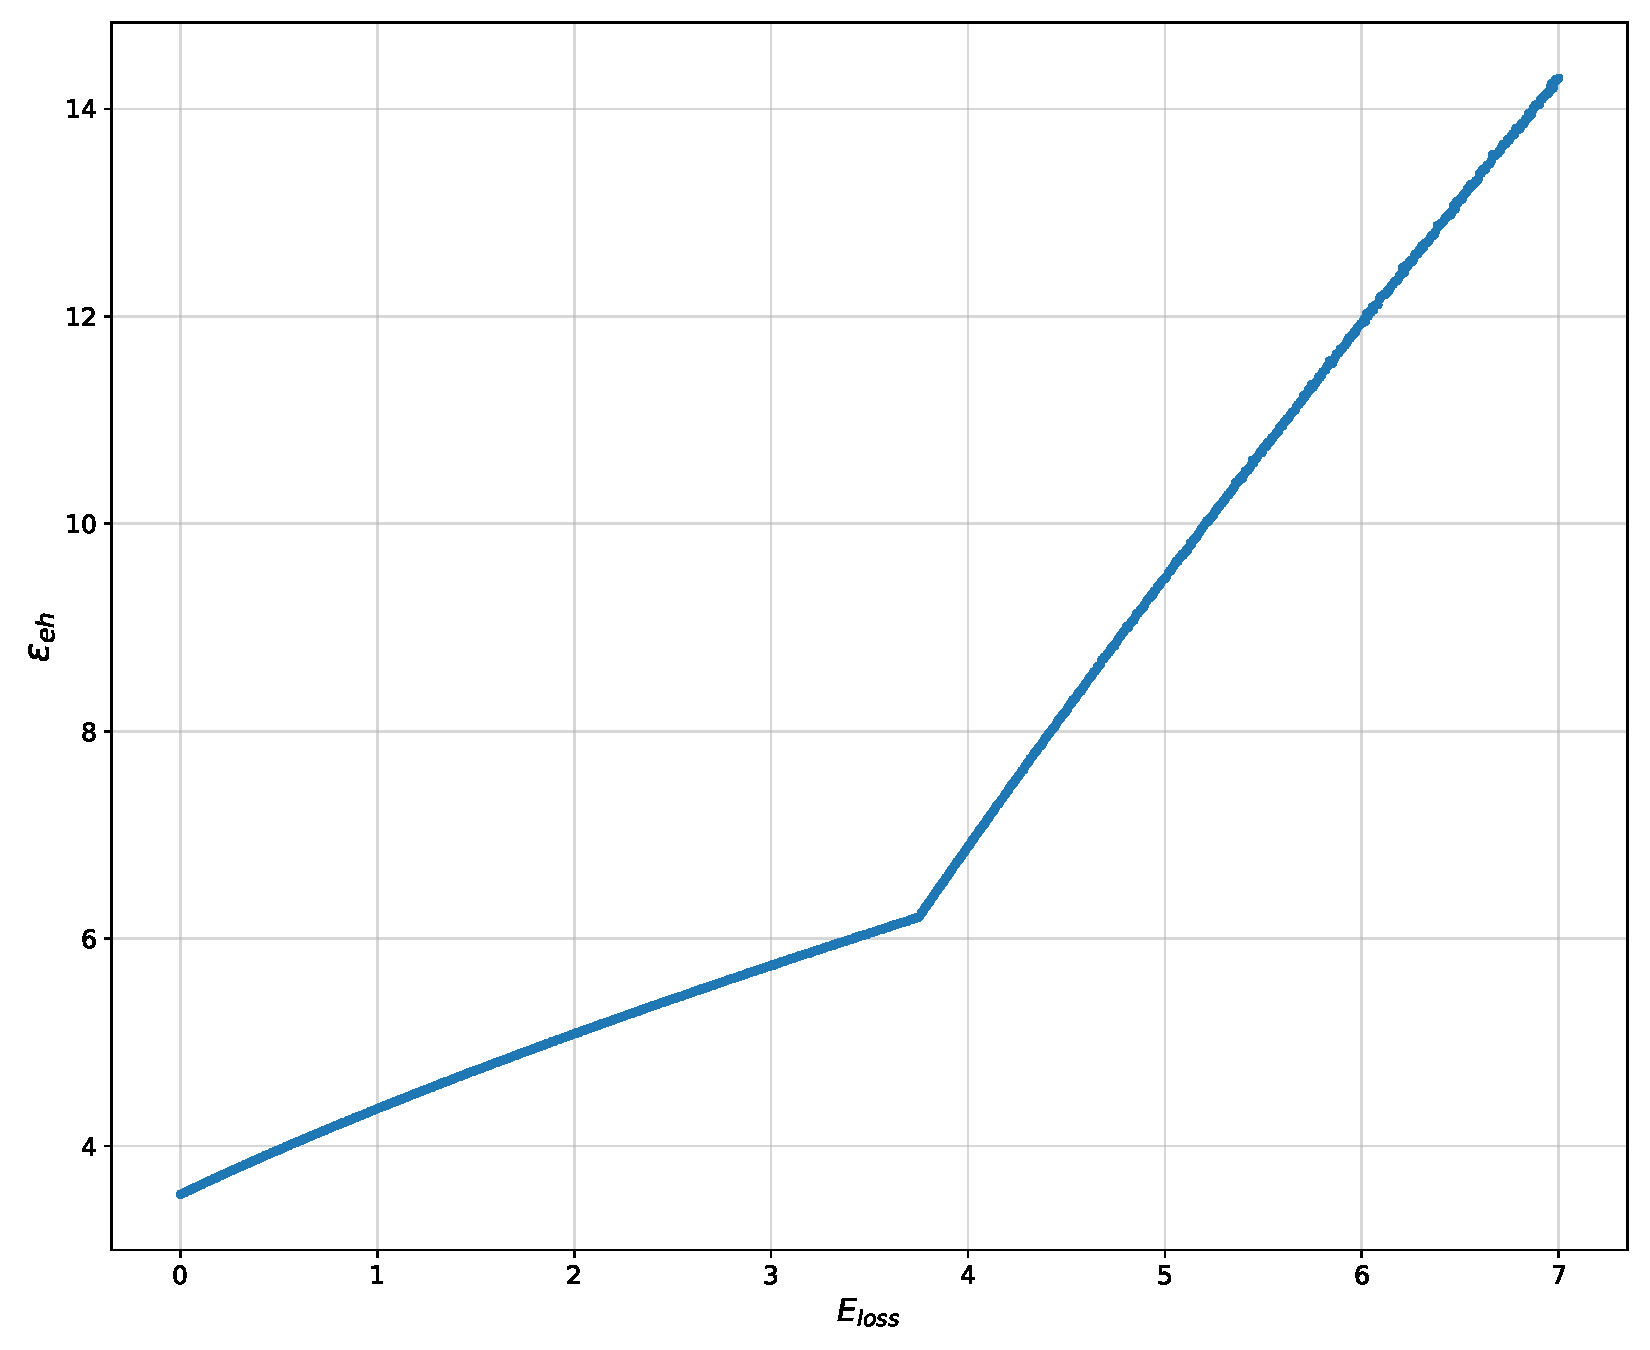
\includegraphics[scale=0.35]{Figs/E_eh_vs_Eloss_5ktrials_0-7Eloss.pdf}
    \caption{\footnotesize{asd.}}
    \label{fig:CreacionHuecoVsEloss}
\end{figure}
Con lo cual se observa que este Montecarlo \textit{de juguete} es muy sensible a dos parámetros muy importantes de la física real del sistema: La energía de creación electrón hueco, porque es el parámetro de la condición de \verb|evolucionar()| que determina si hay o no ionización; y la conservación de la energía. Se observa que cuando la energía se conserva en la simulación, se obtienen los resultados más cercanos a los observados experimentalmente y reportados en la bibliografía.
	
	\pagebreak

    %\addcontentsline{toc}{chapter}{Bibliografía}
    \bibliography{Bibliografia}% Produces the bibliography via BibTeX.
    \bibliographystyle{unsrt}% Produces the bibliography via BibTeX.
    
    \pagebreak
    %\pagestyle{empty}
    
\end{document}
